%%% Time-stamp: <mainrep.tex 19:57, 17 Jul 2016 by P Sunthar>
%%% $Log:$
% This document describes how to use iitbreport style
%********************************************************************

%\documentclass[11pt,a4paper,openright]{report}
\documentclass[twoside]{iitbreport}

%% Default spacing: 1.5
%% Default font size: 12pt
%% Default font: cmr

%%%%%%%%%%%%%%%%%%%%%%%%%%%%%%%%%%%%%%%%%%%%%%%%%%%%%%%%%%%%%%%%%%%%%
%% Prelims from RevelioBP paper

% \usepackage{cite}
% \usepackage{amsmath,amssymb,amsfonts}
% \usepackage{algorithmic}
\usepackage{algorithm} 
\usepackage[noend]{algpseudocode} 
\usepackage[export]{adjustbox}
% \usepackage{graphicx}
\usepackage{textcomp}
\usepackage{bmpsize}
% \usepackage[dvipsnames]{xcolor}
\usepackage{lipsum}
\usepackage{longtable}
\usepackage{cryptocode}
\usepackage{framed}
\usepackage{fancybox}
\usepackage{array}
\usepackage{mdframed}
\usepackage{enumitem}
\usepackage{nameref}
\usepackage{upgreek}
\usepackage{cases}
\usepackage{multirow}
\usepackage{mathrsfs}
\usepackage{dutchcal}
% \usepackage{eufrak}
\usepackage{bbm}
% \usepackage[T1]{fontenc}
% \usepackage[utf8]{inputenc}
% \usepackage{tgadventor}
\usepackage[symbol]{footmisc}
\usepackage{caption,subcaption}
% \usepackage{subfigure}


\usepackage{pgfplots}
\pgfplotsset{compat=1.9}
\usetikzlibrary{spy}
\usetikzlibrary{external}
\usepgfplotslibrary{groupplots}
\tikzexternalize[prefix=plots/]

% \usepackage[colorlinks=true,urlcolor=black]{hyperref}

\newtheorem{theorem}{Theorem}
\newtheorem{lemma}{Lemma}
\newtheorem{corollary}{Corollary}
\newtheorem{definition}{Definition}

\usepackage{chngcntr}
\counterwithin{theorem}{chapter}
\counterwithin{definition}{chapter}
\counterwithin{lemma}{chapter}
% \counterwithin{corollary}{chapter}

\def\BibTeX{{\rm B\kern-.05em{\sc i\kern-.025em b}\kern-.08em
    T\kern-.1667em\lower.7ex\hbox{E}\kern-.125emX}}




%%%%%%%%%%%%%%%%%%%%%%%%%%%%%%%%%%%%%%%%%%%%%%%%%%%%%%%%%%%%%%%%%%%



%% Selectively comment out sections that you want to be left out but
%% maintaining the page numbers and other \ref
\includeonly{%
  intro/introduction,
  prelims/crypto_prelims,
  revelioBP/reveliobp,
  grin-ub/grin_ub,
  lit/literature,
  expt/experimental,
  rnd/results, 
  dec,abs,pub,ack,appendix
}

%%% Some commonly used packages (make sure your LaTeX installation
%%% contains these packages, if not ask your senior to help installing
%%% the packages)

\usepackage{booktabs}
\graphicspath{{expt/}}

%%% Multibib package to be used for listing own publications.
\usepackage[resetlabels]{multibib}
\newcites{Pub}{List of Publications}


%%% Macro definitions for Commonly used symbols
\newcommand{\Rey}{\ensuremath{\mathrm{Re}}}
\newcommand{\avg}[1]{\ensuremath{\overline{#1}}}
\newcommand{\tenpow}[1]{\ensuremath{\times 10^{#1}}}
\newcommand{\pder}[2]{\ensuremath{\frac{\partial#1}{\partial#2}}}

% new \oset macro
\makeatletter
\newcommand{\oset}[3][0ex]{%
  \mathrel{\mathop{#3}\limits^{
    \vbox to#1{\kern-2\ex@
    \hbox{$\scriptstyle#2$}\vss}}}}
\makeatother

\newcounter{mylabelcounter}

\makeatletter
\newcommand{\labelText}[2]{%
#1\refstepcounter{mylabelcounter}%
\immediate\write\@auxout{%
  \string\newlabel{#2}{{1}{\thepage}{{\unexpanded{#1}}}{mylabelcounter.\number\value{mylabelcounter}}{}}%
}%
}
\makeatother

\newcommand\blfootnote[1]{%
  \begingroup
  \renewcommand\thefootnote{}\footnote{#1}%
  \addtocounter{footnote}{-1}%
  \endgroup
}

\newcommand{\vecb}[1]{\oset[-0.4ex]{\rightharpoonup}{\textbf{#1}}}
\newcommand{\vecnb}[1]{{\boldsymbol{#1}}}
\newcommand{\rgen}{\oset[1pt]{\hspace{3mm}\$}{\leftarrow}}


\newcommand{\Plus}{\raisebox{.20ex}{\normalsize\bf +}}
\newcommand{\plus}{\raisebox{.24ex}{\footnotesize +}}
\newcommand{\ToDo}[1]{[\textcolor{blue}{ToDo}: #1]}
\newcommand{\Rplus}{\RBw}
\newcommand{\RPlus}{\RB}
\newcommand{\proto}{$\Uppi_{\RBmath}$ }
\newcommand{\protow}{$\Uppi_{\RBmath}$}

\newcommand{\lang}{$\L_{\RBmath}$ }
\newcommand{\langw}{$\L_{\RBmath}$}

\newcommand{\R}{\textnormal{{\small \fontfamily{qag}\selectfont Revelio}} }
\newcommand{\RB}{\textnormal{{\small \fontfamily{qag}\selectfont RevelioBP}} }
\newcommand{\RBmath}{\textnormal{{\scriptsize \fontfamily{qag}\selectfont RevBP}} }
\newcommand{\Rw}{\textnormal{{\small \fontfamily{qag}\selectfont Revelio}}}
\newcommand{\RBw}{\textnormal{{\small \fontfamily{qag}\selectfont RevelioBP}}}
 
\newcommand{\N}{\mathbb{N}}
\newcommand{\F}{\mathbb{F}}
\newcommand{\E}{\mathscr{E}}
\newcommand{\Inf}{\mathcal{O}}
\newcommand{\Emat}{\mathbcal{E}}
\newcommand{\lvec}{\mathbcal{l}}
\newcommand{\rvec}{\mathbcal{r}}
\newcommand{\Z}{\mathbb{Z}}
\newcommand{\G}{\mathbb{G}}
\newcommand{\Rn}{\mathbb{R}}
\renewcommand{\P}{\mathcal{P}}
\newcommand{\V}{\mathcal{V}}
\newcommand{\C}{\mathcal{C}}
\renewcommand{\L}{\mathcal{L}}
\newcommand{\D}{\mathcal{D}}

\newcommand{\qed}{$\blacksquare$}

\newcommand{\protocolStart}{\begin{itemize}[leftmargin=*]}
\newcommand{\protocolEnd}{\end{itemize}}

\setlist[itemize]{leftmargin=0mm}
\setlist[enumerate]{leftmargin=1cm}

\newcommand{\pointsStart}{\begin{itemize}[leftmargin=*]}
\newcommand{\pointsEnd}{\end{itemize}}

\renewcommand{\thefootnote}{\fnsymbol{footnote}}
\colorlet{lightblue}{Blue!40}


\newtheorem{defn}{Definition}[section]


% Referencing macros
\newcommand{\Eqref}[1]{Equation~\eqref{#1}}
\newcommand{\Tabref}[1]{Table~\ref{#1}}
\newcommand{\Figref}[1]{Figure~\ref{#1}}
\newcommand{\Appref}[1]{Appendix~\ref{#1}}


\begin{document}
	
%%********************************Frontmatter***********************
% In frontmatter everything comes with roman numbering	
\pagenumbering{roman}
\setcounter{page}{1}

%*******************************************************************
%                         Title Page                            
%*******************************************************************
\title{Shorter, Privacy-Preserving Proof of Reserves Protocols for Cryptocurrency Exchanges}
\author{Suyash Bagad}

%% Print the date. Today's date comes by default, change it here to 
%% other date format, if required:

%\date{\today}
%\date{10 Mar 2016}


%% The type of the report can be set here

\reporttype{A Seminar Report}
%\reporttype{A Thesis}
%\reporttype{A Dissertation}
%\reporttype{A Project Report}

%% Name of the degree
\degree{Dual Degree (B.Tech \& M.Tech) in Electrical Engineering with Specialization in Communication \& Signal Processing}
%\degree{Master of Technology}


%% Department/Centre Name
\dept{Department of Electrical Engineering}

%% Supervisor and cosupervisor/excosupervisor are not essential parts
%% of a report title page, as it is your report!

%% But if you **have** to put it uncomment these
\supervisor{Prof. Saravanan Vijayakumaran}
%\cosupervisor{Co-super name}
% \excosupervisor{External Supervisor}

%% Roll number
\rollnum{Roll No. 15D070007}

\maketitle

%*******************************************************************
%                         Copyright Page                          
%******************************************************************* 
%\mycopyright                    

%*******************************************************************
%                         Dedication Page                         
%*******************************************************************
\dedication[Dedicated to \ldots]        
%\addintoc{Dedication}

%*******************************************************************
%                        Certificate Page                         
%*******************************************************************
%\makecertificate[change title name]{report type} 
% \makecertificate{seminar report} 
%\makecertificate{thesis}
\makecertificate{dissertation}
%\makecertificate{project report}

%\addintoc{Certificate}

%*******************************************************************
%                         Approval Sheet                         
%*******************************************************************
%\makeapproval{thesis}
%\makeapproval{dissertation}

%*******************************************************************
%                          Declaration                           
%*******************************************************************
\include{dec} 
%\addintoc{Declaration}

%******************************************************************
%                          Abstract                             
%******************************************************************  
%============================= abs.tex================================
\begin{Abstract}
The rise of cryptocurrencies began with the inception of Bitcoin in 2009. Since
then, several cryptocurrencies with better privacy and security guarantees are being
developed. Cryptocurrencies gained popularity among general masses with the establishment of cryptocurrency exchanges.
Also known as digital currency exchanges or crypto exchanges, they are essentially businesses that allow customers to trade
cryptocurrencies or digital currencies for other assets including conventional fiat
money or different digital currencies. 
From a customer point of view, exchanges not only made owning cryptocurrencies possible to non-miners but also provided them with fast trading platforms for transactions within cryptocurrencies and fiat.
Customers were also provided with custodial wallets freeing them from the hassle of storing and remembering private keys.
In the early days of cryptocurrency, crypto exchanges were very few and less-known, but not too long ago their number increased dramatically and they became an integral part of the cryptoeconomic ecosystem. 
They were responsible for the boost in the transaction volumes of the vast majority of the cryptocurrency sales and liquidity.

The downside of such cryptocurrency exchanges is that they are required to
store sensitive information of customers like the private keys and account balances.
If in case an exchange is hacked, it might result in loss of customer-owned cryptocurrency assets.
There have been many high-profile hacks over the years, many of which went unnoticed for some time \cite{Cryptohacks}.
Although having a fool-proof method to avoid such hacks might be a difficult task, proof of reserves is one way to uphold the trust of customers.
A proof of reserves is the guarantee by the exchange that it owns reserves at least as much as its total liabilities towards customers. 
In this way, even after cases of hacking, the exchange could repay its liabilities to the customers.

The simplest way to publish a proof of reserves for an exchange is to reveal all the addresses or account details it owns so that the customers are convinced about the assets owned by the exchange.
Another way could be to send all the reserves it owns from all its addresses to a single addresses it owns.
If amounts involved in a transaction are public as in the case of Bitcoin, such a self-transaction would be a proof of the exchange's reserves.
For example, in 2011, Mt.~Gox cryptocurrency exchange transferred 424,242 bitcoins from its wallets to a previously revealed Bitcoin address \cite{MtGoxWikipedia}.
However, such proofs of reserves do not preserve the privacy of the exchanges. 
Information of an exchange's addresses or accounts and the total assets it owns are crucial for aspects of its business.
Exchanges naturally would not be in a position to compromise such critical information as a part of proofs of reserves.
The main challenge in design of proofs of reserves is to preserve privacy and confidentiality of exchanges but at the same time convince customers about an exchange's actual asset ownership.
Regaining \textit{trust} of the customers without compromising exchanges' \textit{privacy} is the primary motivation behind the design of better proofs of reserves. 
Advanced cryptographic techniques make it possible to design proofs of reserves which reveal \textit{nothing} beyond an assertation of the form:
\begin{center}
    \textit{Exchange X owns ? amount of the cryptocurrency Y.}
\end{center}
Note that here we do not intend to reveal even the total amount. 
A publicly verifiable proof backing up such a claim is a cryptographic tool known as a \textit{Non-Interactive Zero-Knowledge} proof.

In this work, we study the existing proof of reserves protocols for privacy-centric cryptocurrencies Grin, Beam and Monero.
The existing proof of reserves protocols possess some shortcomings which becomes a hurdle in their practical deployment.
With an aim to alleviate limitations of previously designed proofs of reserves, we design novel proofs of reserves for crypto exchanges supporting the above cryptocurrencies.
Our protocols are shorter and privacy enhancing in comparison to the existing state-of-the-art proofs of reserves.
Previous state-of-the-art proofs of reserves protocols provided some privacy to exchanges by hiding the exchange-owned addresses (or outputs) in a larger anonymity set. 
The proof sizes for these protocols scaled linearly with the anonymity set size.
Since the level of privacy in a proof of reserves directly depends on how large the size of the anonymity set size is as compared to the number of exchange-owned addresses, larger anonymity sets imply stronger privacy.
However, as the previous protocols proof sizes grew linearly as the anonymity set grows, it bought practical limitations (with regards to that of proof storage and broadcast) on what level of privacy could be attained.  
With an aim to improve scalability of the previously design proof of reserves protocols, we design a strategy based on Bulletproofs technique \cite{Bunz2018} to design proofs of reserves scaling logarithmically in the anonymity set.
This brings flexibility in the choice of the size of anonymity set and therefore enhances the attainable level of privacy.
Along with this, we also use the concept of \textit{key images} to ensure that different exchanges cannot share their addresses.
The key images subsequently also helps in detecting double-spending of addresses by an exchange.
Going a step further, we also devise a cryptographic technique to enforce different exchanges to publish proofs of reserves corresponding to a same blockchain state, which is absent in previous work.
This ensures that exchanges can publish proofs of reserves only at particular time instances (for example, after each block is mined), preventing them from cheating customers with ambiguous choices of anonymity sets.   
We also implement the protocols we design as well as the previous state-of-the-art protocols for comparison and show feasibility in practical deployment of our protocols.
We believe that our work on proof of reserves could be well adopted by crypto exchanges and benefit several of their customers.
Furthermore, our work also opens up avenues of exploration of establishing trust without compromising privacy or anonymity in a more general setting.
We are hopeful that this work acts as a small but crucial contribution towards the goal of establishing a \textit{trustless, decentralized economy.}
%
%
%
%
%
\end{Abstract}
%=======================================================================

                    

%******************************************************************
%                         Contents list                         
%******************************************************************
%\figurespagefalse
%\tablespagefalse
\makecontents % Creats toc, lof, and lot

%******************************************************************
%                        Notations                              
%******************************************************************
\notations[4cm]{List of Symbols}      

%%********************************Mainmatter***********************
% In mainmatter everything comes with arabic numbering	
\cleardoublepage
\setcounter{page}{1}
\pagenumbering{arabic}

%******************************************************************
%                         Chapters                           
%****************************************************************** 

\newcommand{\etas}{\ensuremath{\eta_{\mathrm{s}}}}


\chapter{Introduction}

The rise of cryptocurrencies have openend up unending possibilities of how minimal or no trust based systems could be established owing to decentralization.
The concept of blockchain was introduced with the founding of Bitcoin by Satoshi Nakamoto \cite{Nakamoto2009}.
Satoshi Nakamoto proposed and implemented idea of a consensus based, trustless, truly peer-to-peer system for financial transactions.  
Notwithstanding an intrumental step towards establishing a decentralized and a trustless system, Bitcoin has several practical limitations with regards to privacy, security and scalability \cite{Conti2018}.   
This led to the development of more privacy and anonymity focussed cryptocurrencies like Monero \cite{Saberhagen2013} and Zcash \cite{Sasson2014}.
Grin \cite{GrinWebsite} and Beam \cite{BeamWebsite} are two relatively new projects which are backed by the MimbleWimble protocol \cite{Poelstra2016} and claim to promise scalability, anonymity and fungibility all at once.
The rise in privacy-centric cryptocurrencies further led to growth in popularity of cryptocurrencies not only among investors but also common people.


\section{What is a Blockchain?}
\label{scn:blockchain}

\subsection{Decentralized Ledger}




\section{Notion of Privacy on a Blockchain}

\section{Cryptocurrency Exchanges \& Security}

\section{Proof of Solvency}

\subsection{Proof of Reserves}
\subsection{Proof of Liabilities}



%%


%%% Local Variables: 
%%% mode: latex
%%% TeX-master: "../mainrep"
%%% End: 

\chapter{Cryptographic Preliminaries}

Before delving into the details of \RPlus protocol, let us equip ourselves with some background knowledge about the math of cryptocurrencies.


\section{Notation}
Let $\mathcal{G} = \{ \G, q, g \}$ be the description of a cyclic group $\G$ of prime order $q$ with generator $g$ of $\G$. Let $h\in \G$ be another random generator of $\G$ such that the discrete logarithm relation between $g$ and $h$ is not known. Let
$\G^n$ and $\Z^n_q$ be the $n$-ary Cartesian powers of sets $\G$ and $\Z_q$ respectively.
%TODO: Check the second part of the following statement.
% Yes, it is.
Group elements which are Pedersen commitments are denoted by uppercase letters and randomly chosen group elements are denoted by lowercase letters.
% TODO: Check if the following statement is true after the rewrite.
% It is true and necessary too. Matrix description not necessary, so removing it.
Bold font denotes vectors.
Inner product of two vectors $\textbf{a}, \textbf{b} \in \Z_q^n$ is defined as $\langle \textbf{a},\textbf{b} \rangle \coloneqq \sum_{i=1}^{n} a_i \cdot b_i$ where $\textbf{a}=(a_1,\dots, a_n), \textbf{b}=(b_1,\dots,b_n)$. Further, Hadamard and Kronecker products are defined respectively as, $\textbf{a} \circ \textbf{b} \coloneqq (a_1 \cdot b_1, \dots, a_n \cdot b_n) \in \mathbb{Z}_q^n$, $\textbf{a} \otimes \textbf{c} \coloneqq (a_1 \textbf{c}, \dots, a_n \textbf{c}) \in \mathbb{Z}_q^{nm}$ where $\textbf{c} \in \mathbb{Z}_q^m$. For a base vector $\textbf{g} = (g_1, \dots, g_n) \in \G^n$, vector exponentiation is defined as $\textbf{g}^{\textbf{a}} = \prod_{i=1}^{n}g_i^{a_i} \in \G$. For a scalar $u \in \Z_q^{\ast}$, we denote its consecutive powers in the form of a vector $\vecnb{u}^{n} \coloneqq (1, u, u^2, \dots, u^{n-1})$.
To represent the exponentiation of all components of a vector $\textbf{a}$ by the same scalar $k \in \Z_q$, we use $\textbf{a}^{\circ k}$ to mean $(a_1^k, a_2^k, \ldots,a_n^{k})$.
If an element $a$ is chosen uniformly from a set $A$, such a choice is denoted by $a \rgen A$.
We denote the relation \emph{Relation} using the specified input and witness as $\{ (Public \ Input; \ Witness): Relation \}$.
We refer to $\mathcal{A}$ as a \textsf{PPT} adversary which is a probabilistic Turing Machine that runs in polynomial time in the security parameter $\lambda$.
An \emph{interactive proof} for the decision problem $\pi$ is described as follows:
\begin{enumerate}
    \item There are two participants, a \textcolor{blue}{prover} $\P$ and a \textcolor{blue}{verifier} $\V$.
    \item The proof consists of a specified number of rounds.
    \item In the beginning, both participants get the same input.
    \item In each round, the verifier challenges the prover, and the prover responds
    to the challenge.
    \item Both the verifier and the prover can perform some private computation.
    \item At the end, the verifier states whether he was convinced or not.
\end{enumerate}


\section{Assumptions}
\begin{defn}[Discrete Log Relation]
    For all PPT adversaries $\mathcal{A}$ and for all $n\ge2$, $\exists$ a negligible function $\mu (\lambda)$ s.t
    \begin{equation*}
        \Pr 
        \Big[
        \begin{tabular}{ll}
             $\G = Setup(1^{\lambda}), g_1, \dots, g_n \leftarrow \ \G$ ;
             &
             \multirow{2}{*}{$\text{:} \exists a_i \neq 0 \wedge \prod_{i=1}^{n} g_{i}^{a_i} = 1$}\\
             $a_1, \dots, a_n \in \ \Z_p \leftarrow \mathcal{A}(\G, g_1, \dots, g_n)$
             & 
        \end{tabular}
        \Big] 
      \leq \mu(\lambda)
    \end{equation*}
   
    \vspace{0.2mm}
\end{defn} 
We say $\prod_{i=1}^{n} g_{i}^{a_i} = 1$ is a non trivial discrete log relation between $g_1, \dots, g_n$. If the Discrete Log Relation assumption stands, it implies that no \textsf{PPT} adversary can find a non-trivial relation between randomly chosen group elements. 

We use additional cryptographic assumptions such as Decisional Diffie-Hellman and its variants as described in \cite{Lai2019}.

\section{Cryptographic Commitments}

\begin{defn}[Commitments]
    A non-interactive commitment consists of two PPT algorithms {\normalfont(Setup, Com)}. For a message $x \in {\normalfont \textbf{M}_{pp}}$ (message space), the algorithm proceeds as follows:
    \begin{itemize}
    \setlength\itemsep{0.3em}
        \item public parameters $pp \leftarrow {\normalfont Setup}(1^{\lambda})$ for security paramter $\lambda$
        \item {\normalfont Com}$_{pp} : {\normalfont \textbf{M}_{pp}} \times {\normalfont \textbf{R}_{pp}} \rightarrow {\normalfont \textbf{C}_{pp}}$, 
        where ${\normalfont \textbf{R}_{pp}}$ is randomness space
        \item $r \leftarrow {\normalfont \textbf{R}_{pp}}$ and compute {\normalfont \textbf{com}} = {\normalfont Com}$_{pp}(x;r)$
    \end{itemize}
\end{defn}

\begin{defn}[Homomorphic Commitments]
    A homomorphic commitment is a non-interactive commitment such that ${\normalfont \textbf{M}_{pp}}$, ${\normalfont \textbf{R}_{pp}}$, ${\normalfont \textbf{C}_{pp}}$ are all abelian groups, and $\forall \ x_1, x_2 \in {\normalfont \textbf{M}_{pp}}, r_1, r_2 \in {\normalfont \textbf{R}_{pp}}$, we have 
\end{defn}
\begin{equation*}
    \text{Com}(x_1; r_1) + \text{Com}(x_2; r_2) = \text{Com}(x_1+ x_2; r_1+r_2)
\end{equation*}

\begin{defn}[Hiding Commitment]
    A commitment scheme is said to be hiding if for all PPT adversaries $\mathcal{A}$, $\exists \mu(\lambda)$, a negligible function such that,  
\end{defn}
\begin{equation*}
        \Bigg|
        \Pr
        \Bigg[
        \begin{tabular}{c | l}
             \multirow{3}{*}{$\textit{b'=b}$} 
             &
             $\textit{pp} \leftarrow \text{Setup}(1^{\lambda})$;\\
             &
             $(\textit{x}_0,x_1) \in \text{\textbf{M}}_{pp}^2 \leftarrow \mathcal{A}(pp), \
             b \leftarrow \{0,1\}, \ 
             r \leftarrow \text{\textbf{R}}_{pp},$ \\
             &
             $\textbf{com} = Com(\textit{x}_b; r),\ b' \leftarrow \mathcal{A}(pp, \ \textbf{com})$
        \end{tabular}
        \Bigg]
        - \frac{1}{2}
        \Bigg|
        \leq \mu(\lambda)
\end{equation*}
\textit{where the probability is over $b', r, Setup \ \text{and} \ \mathcal{A}$. For perfectly hiding schemes, $\mu(\lambda)=0$.}


\begin{defn}[Binding Commitment]
    A commitment scheme is said to be binding if for all PPT adversaries $\mathcal{A}$, $\exists \mu(\lambda)$, a negligible function such that,
\end{defn}
\begin{equation*}
        \Pr 
        \Bigg[
        \begin{tabular}{c | c}
             \multirow{2}{*}{$\text{Com}(\textit{x}_0;r_0)= \text{Com}(\textit{x}_1;r_1) \wedge x_0 \neq x_1$} 
             &
             $\textit{pp} \leftarrow \text{Setup}(1^{\lambda})$,\\
             &
             $\textit{x}_0, x_1, r_0, r_1 \leftarrow \mathcal{A}(pp)$
        \end{tabular}
        \Bigg] 
        \leq \mu(\lambda)
\end{equation*}
\textit{where the probability is over Setup and $\mathcal{A}$. Again, if $\mu(\lambda)=0$ then we say the scheme is perfectly binding.}

\begin{defn}[Pedersen Commitment]
    ${\normalfont \textbf{M}}_{pp}, {\normalfont \textbf{R}}_{pp} = \mathbb{Z}_p$, ${\normalfont \textbf{C}}_{pp} = \mathbb{G}$ of \\order $p$.
    \begin{itemize}
        \item {\normalfont Setup}: $g, h \leftarrow \mathbb{G}$
        \item {\normalfont Com}$(x; r) = (g^x h^r)$
    \end{itemize}
\end{defn}

\begin{defn}[Pedersen Vector Commitment]
    {\normalfont \textbf{M}}$_{pp} = \mathbb{Z}_p^n$, {\normalfont \textbf{R}}$_{pp} = \mathbb{Z}_p$, ${\normalfont \textbf{C}}_{pp} = \mathbb{G}$ of order $p$.
    \begin{itemize}
        \item {\normalfont Setup}: \textbf{g} $= (g_1, \dots, g_n), h \leftarrow \mathbb{G}$
        \item {\normalfont Com}$(\textbf{x} = (x_1, \dots, x_n); r) = (h^r \textbf{g}^{\textbf{x}})$
    \end{itemize}
\end{defn}

The Pedersen vector commitment is \textcolor{blue}{perfectly hiding} and \textcolor{blue}{computationally binding} under the
discrete logarithm assumption.

\section{Zero-Knowledge Arguments of Knowledge}

\subsection{Zero-Knowledge Arguments}

A protocol in which a prover convinces a verifier that a statement
is true \textit{without} revealing any information about why it holds is known as a Zero-knowledge argument. An argument is a proof only if the prover is computationally bounded and some computational hardness holds. Hereafter, we use the terms \textit{proof} and \textit{argument} interchangeably. 

We illustrate the idea of zero-knowledge arguments of proof using the example of \textit{Ali-Baba's secret cave} \cite{jean89}. \footnote{Figure courtesy: \url{https://en.wikipedia.org/wiki/Zero-knowledge_proof}.}

\begin{figure}[h!]
    \centering
    \begin{subfigure}[b]{0.8\textwidth}
    \centering
        \includegraphics[width=0.44\textwidth]{Figures/Zkip_alibaba1.png}
        \label{fig:bc1}
        \caption{Peggy chooses a path uniformly from $A, B$ without Victor knowing.}
    \end{subfigure}
    \\
    \begin{subfigure}[b]{0.8\textwidth}
    \centering
        \includegraphics[width=0.4\textwidth]{Figures/Zkip_alibaba2.png}
        \label{fig:bc2}
        \caption{Victor asks her to come out of the cave from path $A$.}
    \end{subfigure}
    \\
    \begin{subfigure}[b]{0.8\textwidth}
    \centering
        \includegraphics[width=0.4\textwidth]{Figures/Zkip_alibaba3.png}
        \label{fig:bc3}
        \caption{If Peggy had entered from path $A$, she returns trivially. Otherwise, she could open the door using the secret key and return from path $A$.}
    \end{subfigure}
    
    \caption{Example of a zero knowledge proof}
    \label{fig:zkp_alibaba}
    \end{figure}
    
In the above example, Peggy knows the secret word used to open a mysterious door in a cave. The cave is shaped like a horse-hoe. The entrance is on one side and the magic door blocking the opposite side. Victor wants to know whether Peggy knows the secret word; but Peggy, does not want to reveal her knowledge (the secret word) to Victor or to reveal the fact of her knowledge to anyone in the world. 

Peggy and Victor run the protocol described in figure \ref{fig:zkp_alibaba}. Provided she really does know the magic word, and the path she enters and path Victor asks her to come from are same, then it's trivial for Peggy to succeed and Victor to believe that she actually knows the secret key. Further, if the chosen path by Peggy and asked by Victor doesn't match, even then she could open the door and return from a desired path. If they were to repeat this protocol many times, say 15 times in a row, her chance of successfully "guessing" all of Victor's requests would become exponentially small (about three in a lakh).

For zero-knowledge arguments presented in this report, we will consider arguments consisting of three interactive probabilistic polynomial time algorithms $(\text{Setup}, \mathcal{P}, \mathcal{V})$. These algorithms are described by:
\begin{itemize}[label=$\ast$]
    \item Setup: $\sigma \leftarrow \text{Setup}(1^{\lambda})$, $\sigma$ is common reference string
    \item $\mathcal{P}$: prover, $\mathcal{V}$: verifier
    \item Transcript $tr \leftarrow \langle \mathcal{P}, \mathcal{V} \rangle$
    \item $\langle \mathcal{P}, \mathcal{V} \rangle = b$, $b=0$ if the verifier rejects or $b=1$ accepts 
\end{itemize}

Further, we define the relation $\mathcal{R}$ and the CRS-dependent language as:
\begin{align*}
    \mathcal{R} &:= \{ (\sigma, u, w) \in \{0,1\}^{\ast} \times  \{0,1\}^{\ast} \times  \{0,1\}^{\ast}: \ w \ \text{is a witness for}\ u \ | \ \sigma \}\\
    \mathcal{L}_{\sigma} &:=  \{ x \ | \exists w \in (\sigma, u, w) \in \mathcal{R} \}
\end{align*}

So, $\mathcal{L}_{\sigma}$ is essentially the set of statements $x$ that have a witness $w$ in the relation $\mathcal{R}$. 

\subsection{Defining Zero-Knowledge Arguments of Knowledge}
\label{subsec:zka/d_aok}
To mathematically define the notion of zero-knowledge and zero-knowledge arguments, we will provide the necessary definitions below.

\begin{defn}[Argument of Knowledge]
        The triple $(\text{Setup}, \mathcal{P}, \mathcal{V})$ is called an argument of knowledge for relation $\mathcal{R}$ if it is \textcolor{blue}{perfectly complete} and has \textcolor{blue}{computational witness-extended emulation}.
\end{defn}

\begin{defn}[Perfect completeness]
    $(\text{Setup}, \mathcal{P}, \mathcal{V})$ has perfect completeness if for all non-uniform polynomial time adversaries $\mathcal{A}$

    \begin{equation*}
    \Pr 
    \Big[
    \begin{tabular}{c | l}
         \multirow{2}{*}{$(\sigma, u, w) \not \in \mathcal{R} \ or \ 
         \langle \mathcal{P}(\sigma, u, w), \mathcal{V}(\sigma, u) \rangle = 1$}
         & $\sigma \leftarrow \text{Setup}(1^{\lambda})$
         \\
         & 
         $(u, w) \leftarrow \mathcal{A}(\sigma)$
    \end{tabular}
    \Big] 
    = 1
\end{equation*}
\end{defn}

\emph{Perfect completeness} implies that if a statement is actually true, then an honest verifier is convinced with probability $1$ about the truth of the statement by an honest prover.

\begin{defn}[Computational Witness-Extended Emulation]
    $(\text{Setup}, \mathcal{P}, \mathcal{V})$ has witness-extended
    emulation if for all deterministic polynomial time $P^{*}$ there exists an expected polynomial time
    emulator $\mathcal{E}$ such that for all pairs of interactive adversaries $\mathcal{A}_1 , \mathcal{A}_2$ there exists a negligible function
    $\mu (\lambda)$ such that
    
    \begin{multline*}
    \Bigg|
        \Pr
        \Bigg[
        \begin{tabular}{c | l}
             \multirow{3}{*}{$\mathcal{A}_1(tr) = 1$}
             & $\sigma \leftarrow \text{Setup}(1^{\lambda},)$
             \\
             & 
             $(u, s) \leftarrow \mathcal{A}_2(\sigma),$
             \\
             & $tr \leftarrow \langle (\mathcal{P}^{*}(\sigma, u, s), V(u, s) \rangle$
        \end{tabular}
        \Bigg]
        -\\
        \Pr 
        \Bigg[
            \begin{tabular}{l | l}
                \multirow{2}{*}{$\mathcal{A}_1(tr) = 1 \wedge$}
                &
                $\sigma \leftarrow \text{Setup}(1^{\lambda},)$
                \\
                & 
                $(u, s) \leftarrow \mathcal{A}_2(\sigma),$
                \\
                $(tr\ accepted \implies (\sigma, u, w)\in \mathcal{R})$
                &
                $(tr, w) \leftarrow \mathcal{E}^{\mathcal{O}}(\sigma, u)$
           \end{tabular}
           \Bigg]
    \Bigg|
    \leq \mu(\lambda)
    \end{multline*}
    
    where the oracle is given by  $\mathcal{O} = \langle (\mathcal{P}^{*}(\sigma, u, s), V(u, s) \rangle$, and permits rewinding to a specific point and
    resuming with fresh randomness for the verifier from this point onwards. We can also define com-
    putational witness-extended emulation by restricting to non-uniform polynomial time adversaries
    $\mathcal{A}_1$ and $\mathcal{A}_2$.       
    
\end{defn}

\textit{Computational witness-extended emulation} implies that when an adversary produces an argument to convince the verifier with some probability, then we have a corresponding emulator producing identically distributed argument with same probability, but also a witness.

\begin{defn}[Public coin]
    An argument of knowledge  $(\text{Setup}, \mathcal{P}, \mathcal{V})$ is called public coin if all messages sent from the verifier to the prover are chosen uniformly at random and independent of the prover's messages, i.e., the challenges correspond to the verifier's randomness $\rho$.
\end{defn}

\begin{defn}[Zero Knowledge Argument of Knowledge]
    An argument of knowledge $(\text{Setup}, \mathcal{P}, \mathcal{V})$ is zero knowledge if it reveals no information about $w$ apart from what could be deduced from the fact that $(\sigma, u, w) \in \mathcal{R}$.
\end{defn}

An argument of knowledge is zero knowledge if it does not leak information about $w$ apart from what can be deduced from the fact that $(\sigma, u, w) \in \mathcal{R}$. More explicitly, we note that, a zero knowledge argument of knowledge ensures that no \textsf{PPT} adversary (or verifier) can ever recover $w$ given it's relation with $\sigma, u$.

\begin{defn}[Perfect Special Honest-Verifier Zero-Knowledge]
    A public coin argument of knowledge $(\text{Setup}, \mathcal{P}, \mathcal{V})$ is a perfect special honest verifier zero knowledge (SHVZK) argument of knowledge for $\mathcal{R}$ if there exists a probabilistic polynomial time simulator $\mathcal{S}$ such that for all pairs of interactive adversaries $\mathcal{A}_1 , \mathcal{A}_2$
    
    \begin{multline*}
    \Pr
    \Bigg[
    \begin{tabular}{c | l}
        \multirow{3}{*}{$(\sigma, u, w) \in \mathcal{R} \wedge \mathcal{A}_1(tr) = 1$}
         & $\sigma \leftarrow \text{Setup}(1^{\lambda},)$
         \\
         & 
         $(u, w, \rho) \leftarrow \mathcal{A}_2(\sigma),$
         \\
         & $tr \leftarrow \langle (\mathcal{P}(\sigma, u, s), V(\sigma, u; \rho) \rangle$
    \end{tabular}
    \Bigg]
    \\
    =\Pr
    \Bigg[
    \begin{tabular}{c | l}
        \multirow{3}{*}{$(\sigma, u, w) \in \mathcal{R} \wedge \mathcal{A}_1(tr) = 1$}
         & $\sigma \leftarrow \text{Setup}(1^{\lambda},)$
         \\
         & 
         $(u, w, \rho) \leftarrow \mathcal{A}_2(\sigma),$
         \\
         & $tr \leftarrow \mathcal{S}(u, \rho)$
    \end{tabular}
    \Bigg]
    \end{multline*}

\end{defn}

PSHVZK AoK implies that even if an adversary chooses a
distribution over statements and witnesses, it isn't able to
distinguish between simulated transcript and honestly generated
transcript for $u \in \mathcal{L}_{\sigma}$.




\newcommand{\RBtitle}{\textnormal{\big {\fontfamily{qag}\selectfont RevelioBP}} }


\chapter{RevelioBP - Shorter MimbleWimble Proof of Reserves Protocol}
\label{chap:revBP}

\section{Introduction}
A proof of reserves protocol is used by a cryptocurrency exchange to prove that it owns a certain amount of cryptocurrency. If privacy of the amount or outputs owned by the exchange is not an issue, then proving reserves involves a straightforward proof of the ability to spend the exchange-owned outputs (for example, see \cite{BlockstreamProofOfReserves}). Non-private proof of reserves protocols are unlikely to be adopted by exchanges as they may reveal business strategy. Privacy-preserving proof of reserves protocols have been proposed for Bitcoin \cite{Decker2015,Dagher2015}, Monero \cite{Dutta2019a}, and MimbleWimble \cite{Dutta2019b}. In fact, the protocols proposed by Decker \textit{et al} \cite{Decker2015} and Dagher \textit{et al} \cite{Dagher2015} go one step further and give a privacy-preserving proof of solvency, i.e.~they prove that the reserves owned by the exchange exceed its liabilities towards its customers. However, the work in \cite{Decker2015} relies on a trusted hardware assumption. And the proof of liabilities protocol in \cite{Dagher2015} is secure only if every exchange customer checks the proof. In general, it seems that designing proof of reserves protocols is easier than designing proof of liabilities protocols as the former depend only the blockchain state while the latter depend on the exchange's private customer data.
% An exchange can reduce its reported liabilities by censoring its customer list.

Even without a robust proof of liabilities protocol, a privacy-preserving proof of reserves protocol based on homomorphic commitments is valuable. For example, the proof of reserves protocols in \cite{Dagher2015,Dutta2019a,Dutta2019b} generate a Pedersen commitment $C_{\text{res}}$ to the amount of reserves. Exchanges can easily prove that $C_{\text{res}}$ is a commitment to an amount which exceeds a base amount $a_{\text{base}}$. While the base amount may not be exactly equal to the total liabilities of the exchange, it can be based on the trade volume data published by the exchange \cite{Coinmarketcap}. This technique will help early detection of exchange hacks and exit scams. For example, in Februrary 2019 the Canadian exchange QuadrigaCX claimed that it had lost access to wallets containing customer funds due to the death (in December 2018) of their CEO who had sole custody of the corresponding passwords and keys. But an official investigation found that the wallets had been empty since April 2018, several months before the CEO's death \cite{QuadrigaCXEmpty, EYThirdReport}. This discrepancy would have been detected earlier if the exchange had been required to give perioidic proofs of reserves.
% Realising proof of reserves as an important tool in enhancing customer confidence in crypto-exchanges leads us to the need for building better proofs in terms of privacy, scalability and performance.    

MimbleWimble is a design for a scalable cryptocurrency which was proposed in 2016 \cite{Jedusor2016}. Beam and Grin are two implementations of the MimbleWimble protocol which are available on several exchanges \cite{Coinmarketcap}. \R \cite{Dutta2019b} was the first proof of reserves protocol for MimbleWimble coins which provided some privacy to exchanges by hiding the exchange-owned outputs inside an anonymity set of outputs. As the anonymity set is revealed as part of the proof of reserves, a larger anonymity set results in better privacy for the exchange. Since the \R proof size scales linearly with the anonymity set, it becomes an impediment in scaling the anonymity set to the set of all unspent transaction outputs (UTXOs).
To solve the scalability issue of \Rw, we designed \RB leveraging the Bulletproofs \cite{Bunz2018} framework, resulting in the proof size being logarithmic in the anonymity set size.\\[-6pt]   

\noindent \textbf{Our Contribution.} In this paper, we present \Rplus, a proof of reserves protocol for MimbleWimble with proof sizes scaling \textit{logarithmcally} in the size of the anonymity set and \textit{linearly} in the size of the exchange-owned output set.
This makes it feasible to choose the anonymity set to be the set of all UTXOs on the blockchain.  
To make quantitative comparisons, we have implemented \RB  in Rust.
At the time of writing this paper, the number of UTXOs on the Grin blockchain is approximately 161,000 \cite{GrinScanWebsite}.
A \R proof of reserves for this anonymity set will have size 42 MB as against 0.27 MB using \RPlus instead.\footnote{Under the assumption that the exchange owns 5\% of all UTXOs.}
This reduction in proof size, however, comes at the cost of larger proof generation and verification times. If an exchange is willing to compromise on the size of the proof and is required to give frequent proofs of reserves,
\R serves as a better choice. If proof sizes are critical for an exchange and it is willing to spend more time generating the proof, \RB clearly outperforms \Rw.   
In conclusion, we quantitatively highlight the trade-off between proof size and performance in using \R and \RBw, both of which are based on the discrete log assumption.
% The design of \RPlus is heavily inspired by the recent Omniring proposal for Monero ring confidential transactions by Lai \textit{et al} \cite{Lai2019}, which itself is based on Bulletproofs \cite{Bunz2018}.

%
%
%
\vspace{-2pt}
\section{Preliminaries}
\vspace{-4pt}
%Before delving into the details of our protocol, we include a necessary primer in this section to help understand the protocol better.
\subsection{Notation}
Let $\mathcal{G} = \{ \G, q, g \}$ be the description of a cyclic group $\G$ of prime order $q$ with generator $g$ of $\G$. Let $h\in \G$ be another random generator of $\G$ such that the discrete logarithm relation between $g$ and $h$ is not known. Let
$\G^n$ and $\Z^n_q$ be the $n$-ary Cartesian products of sets $\G$ and $\Z_q$ respectively.

Group elements which are Pedersen commitments are denoted by uppercase letters and randomly chosen group elements are denoted by lowercase letters.

Bold font denotes vectors.
Inner product of two vectors $\textbf{a}, \textbf{b} \in \Z_q^n$ is defined as $\langle \textbf{a},\textbf{b} \rangle \coloneqq \sum_{i=1}^{n} a_i \cdot b_i$ where $\textbf{a}=(a_1,\dots, a_n), \textbf{b}=(b_1,\dots,b_n)$. Further, Hadamard and Kronecker products are defined respectively as, $\textbf{a} \circ \textbf{b} \coloneqq (a_1 \cdot b_1, \dots, a_n \cdot b_n) \in \mathbb{Z}_q^n$, $\textbf{a} \otimes \textbf{c} \coloneqq (a_1 \textbf{c}, \dots, a_n \textbf{c}) \in \mathbb{Z}_q^{nm}$ where $\textbf{c} \in \mathbb{Z}_q^m$. For a base vector $\textbf{g} = (g_1, \dots, g_n) \in \G^n$, vector exponentiation is defined as $\textbf{g}^{\textbf{a}} = \prod_{i=1}^{n}g_i^{a_i} \in \G$. For a scalar $u \in \Z_q^{\ast}$, we denote its consecutive powers in the form of a vector $\vecnb{u}^{n} \coloneqq (1, u, u^2, \dots, u^{n-1})$.
To represent the exponentiation of all components of a vector $\textbf{a}$ by the same scalar $k \in \Z_q$, we use $\textbf{a}^{\circ k}$ to mean $(a_1^k, a_2^k, \ldots,a_n^{k})$.
If an element $a$ is chosen uniformly from a set $A$, such a choice is denoted by $a \rgen A$.
For a positive integer n, let $[n]$ denote the set $\{1,2,\dots,n\}$.

\subsection{Outputs in MimbleWimble}

In MimbleWimble, coins are stored in outputs which consist of Pedersen commitments of the form $C = g^rh^a\in \G$ where $g , h \in \G$ and $r,a \in \Z_q$. Here $a$ represents the amount of coins stored in the output and $r$ is a blinding factor. Each commitment is accompanied by a range proof which proves that the amount $a$ lies in the range $\{0,1,2,\ldots,2^{64}-1\}$.

The group elements $g$ and $h$ are assumed to have an unknown discrete logarithm relationship. For example, in Grin $\G$ is the secp256k1 elliptic curve group, $g$ is the base point of the secp256k1 curve, and $h$ is obtained by hashing $g$ with the SHA256 hash function \cite{RustSecp256k1Constants}. The unknown discrete logarithm relationship makes the commitment computationally binding, i.e.~a polynomial-time adversary cannot find $r' \neq r$ and $a' \neq a$ such that $C = g^rh^a = g^{r'}h^{a'}$.

To spend an output having the commitment $C = g^r h^a$, knowledge of the blinding factor $r$ is required \cite{GrinDocOnGithub}. As spending ability is equivalent to ownership, a proof of reserves protocol for MimbleWimble involves a proof of knowledge of blinding factors of several outputs.

\vspace{-2pt}
\subsection{From Omniring to \textnormal{{\fontfamily{qag}\selectfont RevelioBP}}}
In Monero, source addresses in a transaction are obfuscated using ring signatures and the amounts are hidden in Pedersen commitments \cite{Noether2016}. 
%The transaction structure, called \textit{ring confidential transaction (RingCT)}, proves that (a) the transaction creator knows one of the private keys corresponding to the public keys in the ring, (b) the sum of the amounts in the input Pedersen commitments is equal to the sum of the amounts in the output Pedersen commitments plus transaction fees, and (c) the output Pedersen commitments contain amounts in a valid range.
The current transaction structure in Monero, called \textit{ring confidential transaction (RingCT)}, has proof sizes which scale linearly in the ring size. Omniring \cite{Lai2019} is a recent proposal for RingCTs with proof sizes which scale logarithmically in the ring size. It relies on Bulletproofs \cite{Bunz2018} to achieve this size reduction. Given a ring $\mathcal{R} = (R_1, R_2,\ldots,R_n)$ of public keys where $R_i = h^{x_i}$ for $h \in \G, x_i \in \Z_q$, the Omniring construction enables a prover to prove knowledge of the private keys $x_{i_1}, x_{i_2},\ldots,x_{i_m}$ corresponding to a subset $\mathcal{R}_{\mathcal{S}}$ of $\mathcal{R}$ without revealing $\mathcal{R}_{\mathcal{S}}$. For each public key $R_j$ in this subset $\mathcal{R}_{\mathcal{S}}$, the prover also outputs a \textit{tag} given by $\textsl{tag}_j = g^{x_j^{-1}}$ for $g \in \G$. This tag is used to detect double spending from a source address.

The design of \RB is inspired by the Omniring construction. Given the set of UTXOs $\C_{\text{utxo}}=(C_1,C_2,\ldots,C_n)$ on the blockchain where $C_i = g^{r_i}h^{a_i}$ for some $r_i, a_i \in \Z_q$, the prover in \RPlus proves knowledge of blinding factors $r_i$ and amounts $a_i$ for all $C_i$ in a subset $\C_{\text{own}}$ of $\C_{\text{utxo}}$ without revealing $\C_{\text{own}}$. For each output $C_j \in \C_{\text{own}}$, the prover outputs a tag $\textsl{tag}_j = g_t^{r_j}h^{a_j}$ where $g_t \in \G$ is a randomly chosen group element. In \Rplus, the tag has a dual role. Firstly, it is used to detect output sharing between exchanges. Secondly, the product of the tags is a Pedersen commitment to the total reserves of the exchange.

\vspace{-1pt}
\section{\textnormal{{\fontfamily{qag}\selectfont RevelioBP}} Proof of Reserves Protocol}
\label{scnSecurityPropertiesDefiniton}
%In MimbleWimble, coins are stored in outputs which consist of Pedersen commitments of the form $C = g^rh^a\in \G$ where $g , h \in \G$ and $r,a \in \Z_q$.
%Here $a$ represents the amount of coins stored in the output and $r$ is a blinding factor.
%The group elements $g$ and $h$ are assumed to have an unknown discrete logarithm relationship.
%Each commitment is accompanied by a range proof which proves that the amount $a$ lies in a range like $\{0,1,\ldots,2^{64}-1\}$.

To spend a MimbleWimble output having the commitment $C = g^r h^a$, knowledge of the blinding factor $r$ is required \cite{GrinDocOnGithub}.
%As spending ability is equivalent to ownership, a proof of reserves protocol for MimbleWimble involves a proof of knowledge of blinding factors of several outputs.
Technically, the ability to spend an output also requires knowledge of the amount $a$. But the amount can be at most $2^{64}-1$, and hence can be found by brute force search given $C$ and $r$.

Let $\C_{\text{utxo}}^t$ be the set of UTXOs on a MimbleWimble blockchain after the block with height $t$ has been mined. An exchange will own a subset $\C_{\text{own}}^t \subset \C_{\text{utxo}}^t$, where ownership implies knowledge of the blinding factor for each output $C \in \C_{\text{own}}^t$.  Using the \RB protocol, the exchange can construct a Pedersen commitment $C_{\text{res}}$ to an amount which is equal to the sum of the amounts commited to by each of the outputs in $\C_{\text{own}}^t$.  Given a Pedersen commitment $C_{\text{liab}}$ to the total liabilities of the exchange, it can give a proof of solvency via a range proof which shows that the amount committed to in $C_{\text{res}}C_{\text{liab}}^{-1}$ is non-negative. If there is no suitable method to construct $\C_{\text{liab}}$, then the exchange can reveal a base amount $a_{\text{base}}$ and prove that $\C_{\text{res}}h^{-a_{\text{base}}}$ is a commitment to a non-negative amount.

While \RPlus does not reveal $\C_{\text{own}}^t$, it does reveal its cardinality $s_t = \left| \C_{\text{own}}^t \right|$.
% While this may seem like a privacy concern, an exchange can create some outputs which have zero amount in them for the purpose of \textit{padding} the cardinality.
We give a reasonable workaround for this issue in Section \ref{scnProofGeneration}.



%% Briefly state the properties of Revelio+
If the Decisional Diffie-Hellman (DDH) assumption holds in the group $\G$, the \RPlus proof of reserves protocol satisfies the following properties:
\pointsStart
\item \textit{Inflation resistance}: Using \RBw, a probabilistic polynomial time (\textsf{PPT}) exchange will not be able to generate a commitment to an amount which exceeds the reserves it actually owns.% Moreover, the exchange also cannot generate a commitment to an amount lesser than what it owns prohibiting under-reporting of reserves.
\item \textit{Collusion detection}: Situations where two exchanges share an output while generating their respective \RPlus proofs will be detected.
\item \textit{Output privacy}: A \textsf{PPT} adversary who observes \RPlus proofs from an exchange cannot do any better than random guessing while identifying members of $C_{\text{own}}^t$.
\pointsEnd

The security proofs are given in Section \ref{scnSecurityProperties}.

\subsection{Proof Generation}
\label{scnProofGeneration}
The \RPlus protocol requires one randomly chosen group element $g_t \in \G$ per block such that the discrete log relation between $g_t$ and $g,h$ is unknown.
All the exchanges need to agree upon the procedure used to generate the sequence of $g_t$s.
For example, $g_t$ could be generated by hashing the contents of the block at height $t$. An exchange giving a \RPlus proof of its reserves at the block with height $t$ performs the following procedure:
\begin{enumerate}[itemsep=3pt]
  \item From the UTXO set $\C_{\text{utxo}}^t$ at block $t$, the exchange constructs the vector $\textbf{C} = (C_1,C_2,\dots, C_n)$ where the $C_i$s are all the UTXOs arranged in the order of their appearance on the blockchain. So $n = \left| \C_{\text{utxo}}^t \right|$.
  To keep the notation simple, we do not make the dependence of $\textbf{C}$ and $n$ on $t$ explicit.
  \item The exchange owns a subset $\C_{\text{own}}^t = \{C_{i_1}, C_{i_2},\ldots,C_{i_s}\}$ of $\C_{\text{utxo}}^t$ where $1 \le i_1 < \cdots < i_s \le n$.
  % Once again, we suppress the dependence of $s$ on $t$ for notational simplicity.
  For each $C_{i_j} \in \C_{\text{own}}^t$, the exchange knows $r_{j}$ and $a_{j}$ such that $C_{i_j} = g^{r_j}h^{a_j}$.
  Using this information, the exchange constructs the \textit{tag vector} $\textbf{I} = (I_1, I_2, \ldots, I_s)$ where $I_j = g_t^{r_j}h^{a_j}$.
  Note that $I_j$ is a Pedersen commitment to the amount $a_{j}$ with blinding factor $r_{j}$ using bases $g_t$, $h$.
  So the only difference between $C_{i_j}$ and $I_j$ is that the base $g$ in the former is replaced with $g_t$ in the latter.

  \item Let $\textbf{a} = (a_1,a_2,\ldots,a_s)$ and $\textbf{r} = (r_1, r_2, \ldots,r_s)$ be the amount and blinding factor vectors corresponding to the exchange-owned outputs. Let $\textbf{e}_{i_j} \in \{0,1\}^n$ be the unit vector with a $1$ in position $i_j$ and $0$s everywhere else. Let $\Emat \in \{0,1\}^{s \times n}$ be the matrix with $\textbf{e}_{i_1},\textbf{e}_{i_2},\ldots,\textbf{e}_{i_s}$ as rows.

  The exchange publishes $(t, \textbf{I})$ and generates a zero-knowledge argument of knowledge \proto of quantities $(\Emat, \textbf{a}, \textbf{r})$ such that for all $j=1,2,\ldots,s$
  \begin{equation}
    \textbf{C}^{\textbf{e}_{i_j}} = g^{r_j}h^{a_j}, \ I_j = g_t^{r_j}h^{a_j}.
    \label{eqnTagConstruction}
  \end{equation}
 

  \item The exchange publishes its \RPlus proof as $\left(  t, \textbf{I}, \Uppi_{\RBmath} \right)$ and claims that $C_{\text{res}} = \prod_{j=1}^s I_j$ is a Pedersen commitment to its reserves $\sum_{j=1}^{s}a_j$.
\end{enumerate}
Note that the tag $I_j$ is a deterministic function of the output $C_{i_j}$ at a given block height $t$. So if two exchanges try to use the same output in their respective \RPlus proofs, the same tag $I_j$ will appear in both their proofs, revealing the collusion.

The reason for changing the base $g_t$ with the block height is to change the tag of the same output across \RPlus proofs at different block heights. If $g_t$ were unchanged (as in \R \cite{Dutta2019b}), then the appearance of the same tag in two \RPlus proofs at different block heights will reveal that some exchange-owned output has remained unspent between these two block heights.

As $C_\text{res}$ is a Pedersen commitment with respect to bases $g_t$ and $h$, the Pedersen commitment $C_{\text{liab}}$ to the exchange's liabilities should also be generated using these bases. Otherwise, it will be not be possible to generate a range proof on $C_{\text{res}}C_{\text{liab}}^{-1}$.

The proof reveals the cardinality $s$ of $\C_{\text{own}}^t$. 
An exchange which wants to hide the number of outputs it owns can create some outputs which commit to the zero amount and use these to pad the outputs with non-zero amounts.
For example, suppose that the number of outputs owned by the exchange is expected to be in the range 600 to 1000. It can create 400 outputs which commit to the zero amount and use these to always pad the number $s$ revealed in the proof to be always 1000.
Of course, the exchange would need to spend a nominal amount as transaction fees in creation of such outputs.

Finally, note that an exchange can under-report its reserves by excluding an output it owns from the subset $\C_{\text{own}}^t$ used to generate the \RPlus proof. An exchange may choose to do this if its liabilities are much lower than its reserves.

\subsection{Proof Verification}
Given a \RPlus proof of reserves $(t, \textbf{I}, \Uppi_{\RBmath})$ from an exchange referring to the block height $t$, the verifier performs the following procedure:
\begin{enumerate}[itemsep=3pt]
\item First, it reads the set of all UTXOs at block height $t$ and forms the vector $\textbf{C} = (C_1, \dots, C_n)$ such that $C_i$s are listed in the order of their appearance on the blockchain.

\item It verifies the argument of knowledge $\Uppi_{\RBmath}$ by checking that the verification equations described in Figure \ref{fig:protocol_revBP} hold.

\item Finally, the verifier checks if any of the tags in the $\textbf{I}$ vector appear in another exchange's \RPlus proof for the same block height $t$. If the same tag $I_j$ appears in the \RPlus proofs of two different exchanges, then collusion is declared and the proofs is considered invalid.
\end{enumerate}



\section{ZK Argument of Knowledge \proto}
\label{scnArgumentOfKnowledge}
Let $\textbf{C} = (C_1,\ldots,C_n)$ be the vector representation of the UTXO set $\C_{\text{utxo}}^t$ at block height $t$.
Let $\textbf{I} = (I_1, \ldots, I_s)$ be the tag vector published by the exchange as part of the \RPlus proof.
The exchange constructs an argument of knowledge \proto to convince a verifier of the following:

\begin{enumerate}
  \item[(i)] It knows $r_j$ and $a_j$ such that $I_j = g_t^{r_j}h^{a_j}$ $\forall j \in [s]$.\\[-8pt]
  \item[(ii)] $\exists i_j \in [n]$ (index) such that $C_{i_j} = g^{r_j}h^{a_j}$ $\forall j \in [s]$.
\end{enumerate}
\vspace{1mm}
Note that while the existence of the indices $i_j$ will be proved by \protow, the indices themselves are not revealed. 
Since the term $h^{a_j}$ is common in both equations in the above statements, combining the two equations, 
we can equivalently state that the exchange knows $r_j$ and $i_j$ such the following holds for all $j \in [s]$
\begin{equation}
  I_j g_t^{-r_j} = C_{i_j} g^{-r_j}.
\end{equation}
%
%This is possible because an honest exchange could construct a valid $I_j$ even if it does not know the amount $a_j$.
In other words, knowledge of $r_j$ and $i_j$ for all $j \in [s]$ suffices for an honest exchange to construct \protow.


Consider the language \lang given in (\ref{eqnRevelioPlusLanguage}) where 
$\textbf{r} = (r_1,r_2,\ldots,r_s) \in \Z_q^s$
and $\textbf{e}_{i_j} \in \{0,1\}^n$ is a unit vector with a 1 at index $i_j$ and zeros everywhere else.
The language depends on the common reference string $\textsl{crs}=\{\G, q, g, h, g_t\}$.
\begin{align}
\L_{\RBmath} = \hspace{-1mm}
\left\{ ( \textbf{C}, \textbf{I}) \Bigg| 
\text{
\begin{tabular}{c} 
$\exists (\textbf{r}, \textbf{e}_{i_1},\ldots,\textbf{e}_{i_s}) \text{ such that }$
\\ 
$I_j g_t^{-r_j} = \textbf{C}^{\textbf{e}_{i_j}} g^{-r_j} \ \forall j \in [s]$
\end{tabular}
}
\hspace{-1mm}
\right\}
\label{eqnRevelioPlusLanguage}
\end{align}

To leverage the Bulletproofs framework for the construction of a \textit{log}-sized argument of knowledge for the language
\langw, we need to do the following:

\begin{enumerate}
  \item[(i)] Embed the secrets $(\textbf{r}, \textbf{e}_{i_1},\ldots,\textbf{e}_{i_s})$ as the exponents in a Pedersen vector commitment satisfying some inner product relation.
  \item[(ii)] Using the public information $(\textbf{C}, \textbf{I})$, construct the base vectors of the Pedersen vector commitment in such a way that the prover would not know the discrete logarithm relation between elements of the base vectors.  
\end{enumerate}

The first requirement seems natural since the Bulletproofs technique helps us prove the knowledge of exponents in a Pedersen vector commitment satisfying some inner product relations.
The second one is a more technical requirement. In Bulletproofs, the elements in the base vectors $\textbf{g}, \textbf{h} \in \G^n$ are uniformly chosen from the group $\G$ to ensure 
that a discrete logarithm relation between them is not known to a \textsf{PPT} prover. The soundness of the Bulletproofs protocol relies on this assumption.
Lai \textit{et al} \cite{Lai2019} noted that if base vector components are chosen from a blockchain a prover might know the discrete logarithm relation between them.
To solve this problem, they proposed using a base vector which is the Hadamard product of the vectors taken from the blockchain (with a random exponent) and a randomly chosen base vector.

To construct a base vector satisfying the above requirements, we write the statement of $\mathcal{L}_{\textsf{RevBP}}$ from (\ref{eqnRevelioPlusLanguage}) as 
\begin{gather}
  g^{-r_j} g_t^{r_j} \textbf{C}^{\textbf{e}_{i_j}} I_j^{-1} = 1 \ \forall j \in [s]. \label{eqnCombinedStatement}
  \intertext{For $u \rgen \Z_q$, combining the above constraints, we have}
  \prod_{j \in [s]} \left(g^{-r_j} g_t^{r_j} \textbf{C}^{\textbf{e}_{i_j}} I_j^{-1}\right)^{u^{j-1}} = 1, \nonumber \\
  \hspace{-1.5cm} \implies \hspace{0.8cm} g^{- \langle \vecnb{u}^s, \vecnb{r} \rangle} g_t^{\langle \vecnb{u}^s, \vecnb{r} \rangle} \textbf{C}^{ \vecnb{u}^s \Emat} \textbf{I}^{- \vecnb{u}^s} = 1,
  \label{eqnMainEqualityCompressed}
\end{gather}
where $\Emat$ is a $s \times n$ matrix having the $\textbf{e}_{i_j}$ vectors as rows.
We write the exponents in (\ref{eqnMainEqualityCompressed}) as \textit{compressed secrets},
namely $\xi = -\langle \vecnb{u}^s, \vecnb{r} \rangle, \ \xi^{\prime} = \langle \vecnb{u}^s, \vecnb{r} \rangle, \ \hat{\textbf{e}} = \vecnb{u}^s \Emat$ and let $\hat{I} = \textbf{I}^{-\vecnb{u}^s}$.  
Given a vector $\textbf{p} \in \G^{n+3}$ and a scalar $w \in \Z_q$, we construct the base and exponent vectors as follows
\begin{align}
    \textbf{g}_w^{\prime} & \coloneqq \big( (g\|g_t\|\textbf{C}\| \hat{I})^{\circ w} \circ \textbf{p} \big),
    \label{eqnBaseCompressed} \\
    \textbf{a}^{\prime} & \coloneqq (\xi \| \xi^{\prime} \| \hat{\textbf{e}} \| 1).
    \label{eqnExpCompressed}
\end{align}
Note that the compressed secrets are a linear combination of the actual secrets.
We need to append the actual secrets $(\textbf{r}, \textbf{e}_{i_1}, \dots, \textbf{e}_{i_s})$ for completeness to (\ref{eqnExpCompressed}). Thus, we have
\begin{align}
  \textbf{g}_w & \coloneqq \big[ \big( (g\|g_t\|\textbf{C}\| \hat{I})^{\circ w} \circ \textbf{p} \big) \| \textbf{g}^{\prime} \big],
  \label{eqnBase}\\
  \textbf{a} & \coloneqq \big[ (\xi \| \xi^{\prime} \| \hat{\textbf{e}} \| 1) \| (\textbf{e}_{i_1} \| \dots \| \textbf{e}_{i_s} \| \textbf{r}) \big].
  \label{eqnExp}
\end{align} 
where $\textbf{g}^{\prime} \rgen \G^{sn+s}$.
We now state a lemma in regards to the non-trivial discrete-log relation between the components of the base vector $\textbf{g}_w$.% and prove it in Appendix \ref{proofThmNoDLBase}.
\begin{lemma}\label{thmNoDLBase}
  If the components of $\textbf{p}$ are chosen uniformly from $\G$ and independent of $(\textbf{C}, \textbf{I})$, 
  then a \textsf{PPT} adversary cannot find a non-trival discrete logarithm relation between components of $\textbf{g}_w$.
\end{lemma}
\textit{Proof}: 
As the components of $\textbf{p}$ and $\textbf{g}^{\prime}$ are uniformly chosen from $\G$, the components of $\textbf{g}_w$ are iid with a uniform distribution in $\G$.  
Hence a PPT adversary cannot find a non-trivial discrete logarithm relation between these components.
\hfill {\small \qed}




% Concretely, let us concentrate on proving knowledge of only one unit vector $\textbf{e}_{i_j}$ for some $j \in [s]$ and the corresponding scalar $r_j$. 
% From (\ref{eqnRevelioPlusLanguage}), we can write
% \begin{gather}
%     g^{-r_j} g_t^{r_j} \textbf{C}^{\textbf{e}_{i_j}} I_j^{-1} = 1. \label{eqnCombinedStatement}
%     % \intertext{For $u \rgen \Z_q$, we have}
%     % \left(g^{-r_j} g_t^{r_j} \textbf{C}^{\textbf{e}_{i_j}} I_j^{-1}\right)^u =  g^{-u r_j} g_t^{u r_j} \textbf{C}^{u\textbf{e}_{i_j}} I_j^{-u} = 1.
%     % \label{eqnMainEqualityCompressed}
% \end{gather}
% Given a vector $\textbf{p} \in \G^{n+3}$ and a scalar $w \in \Z_q$, we construct the base and exponent vectors as follows
% \begin{align}
%     \textbf{g}_w^{\prime} & \coloneqq \left((g\|g_t\|\textbf{C}\|I_j^{-u})^{\circ w} \circ \textbf{p} \right),
%     \label{eqnBaseCompressed}\\
%     \textbf{a}^{\prime} & \coloneqq (-r_j \| r_j \| \textbf{e}_{i_j} \| 1).
%     \label{eqnExpCompressed}
% \end{align}

% Note that $(\textbf{g}_w^{\prime})^{\textbf{a}^{\prime}} = (\textbf{g}^{\prime}_{w^{\prime}})^{\textbf{a}^{\prime}}$ for any $w, w^{\prime} \in \Z_q$ owing to the equality in (\ref{eqnCombinedStatement}).
% We now state a lemma in regards to the non-trivial discrete-log relation between the elements of the base vector $\textbf{g}_w^{\prime}$ and prove it in Appendix \ref{proofThmNoDLBase}.

% \begin{lemma}\label{thmNoDLBase}
%   If the components of $\textbf{p}$ are chosen uniformly and independent of $(\textbf{C}, \textbf{I})$, then there is no non-trival discrete logarithm relation between elements in $\textbf{g}_w^{\prime}$.
% \end{lemma}

% \noindent We prove the above lemma in Appendix \ref{proofThmNoDLBase}.
% Further, we can write the exponents in form of a secret vector as 
% % Further, let the \textit{compressed secrets} (exponents) be $\xi_j = -u r_j,\ \xi^{\prime} = u r_j,\ \hat{\textbf{e}}_j = u \textbf{e}_{i_j}$ and let the corresponding vector be
% \begin{equation}\label{eqnExpCompressed}
%   \textbf{a}^{\prime} \coloneqq (-r_j \| r_j \| \textbf{e}_{i_j} \| 1).
% \end{equation}

We can now construct a Pedersen vector commitment as $A = (h^{\prime})^{r}\textbf{g}_w^{\textbf{a}} \textbf{h}^{\textbf{b}}$ for appropriately chosen $\textbf{b} \in \Z_q^{N}, \textbf{h} \rgen \G^{N}$ where $N = |\textbf{a}|$,
satisfying the first requirement in using the Bulletproofs framework.
Owing to (\ref{eqnMainEqualityCompressed}), (\ref{eqnBase}), (\ref{eqnExp}), we have $\textbf{g}_w^{\textbf{a}} = \textbf{g}_{w^{\prime}}^{\textbf{a}}$ for any $w, w^{\prime} \in \Z_q$.
Thus, the above vector commitment to $\textbf{a}$ remains the same for any $w \in \Z_q$. By successfully running the Bulletproofs protocol twice on $A$ with respect to two different bases
$(h^{\prime} \| \textbf{g}_w \| \textbf{h})$ and $(h^{\prime} \| \textbf{g}_{w^{\prime}} \| \textbf{h})$ we can extract the secret vector $\textbf{a}$ such that $A = (h^{\prime})^{r}\textbf{g}_w^{\textbf{a}} \textbf{h}^{\textbf{b}} = (h^{\prime})^{r}\textbf{g}_{w^{\prime}}^{\textbf{a}} \textbf{h}^{\textbf{b}}$.
This solves the problem of extractability (soundness) of the protocol.
In summary, we are now ready to construct a Bulletproofs-based argument of knowledge proving that the exchange some outputs from the entire set of UTXOs.

% To prove knowledge of the exact secrets $(r_j, \textbf{e}_{i_j})$, we append the above base and the exponent vectors with $\textbf{g}^{\prime} \rgen \G^{n+1}$ and $(\textbf{e}_{i_j} \| r_j)$ respectively.
% \begin{align}
%     \textbf{g}_w &\coloneqq \left[((g\|g_t\|\textbf{C}\|I_j^{-u})^w \circ \textbf{p}) \| \textbf{g}^{\prime}\right]. \\
%     \textbf{a} &\coloneqq \left[(\xi_j \| \xi_j^{\prime} \| \hat{\textbf{e}}_j \| 1) \ \| \ (\textbf{e}_{i_j} \| r_j) \right].
% \end{align}

% Using the new base vector $\textbf{g}_{w}$ and secret vector $\textbf{a}$, we can prove the knowledge of $(r_j, \textbf{e}_{i_j})$ using Bulletproofs. 
% % Appealing to a slightly modified version of Lemma \ref{thmNoDLBase}, the elements of the base vector $\textbf{g}_w$ have no non-trival discrete logarithm relation between them.
% In summary, we can now construct a Bulletproofs-based argument of knowledge proving that the exchange owns one output from the entire set of UTXOs.
% To prove the knowledge of multiple such exchange-owned outputs, we use the aggregated Bulletproofs technique to give a consolidated Bulletproofs-like protocol.

% More precisely, to prove the knowledge of $(\textbf{r}, \textbf{e}_{i_1}, \dots, \textbf{e}_{i_s})$, we combine the statements in (\ref{eqnCombinedStatement}), for all $j \in [s]$,
% by raising them to powers of $u \in \Z_q$.
% \begin{gather}
%   \prod_{j=1}^{s} \big( g^{-r_j} g_t^{r_j} \textbf{C}^{\textbf{e}_{i_j}} I_j^{-1}\big)^{u^{j-1}} = 1. \nonumber \\
%   g^{- \sum_{1}^{s} r_j u^{j-1} } \cdot g_t^{\sum_{1}^{s} r_j u^{j-1} } \cdot \prod_{1}^{s} \big( \textbf{C}^{u^{j-1} \textbf{e}_{i_j}} \big)\big( I_j^{-u^{j-1}} \big) = 1. \nonumber
% \end{gather}

% \noindent Using the notation defined in Fig. (\ref{label:notation}), we get 
% \begin{equation}
%   g^{\xi}\cdot g_t^{\xi^{\prime}} \cdot \textbf{C}^{\hat{\textbf{e}}} \cdot \hat{I} = 1.
% \end{equation} 
% \noindent We refer to the above equlity as \textit{main equality}. The base and the exponent vectors become 
% \begin{gather}
%   \textbf{g}_w \coloneqq \left[((g\|g_t\|\textbf{C}\|\hat{I})^w \circ \textbf{p}) \| \textbf{g}^{\prime}\right]. \\
%   \textbf{c}_L \coloneqq \left[(\xi \| \xi^{\prime} \| \hat{\textbf{e}} \| 1) \ \| \ (\Emat \| \vecnb{r}) \right].
% \end{gather}
% \noindent where $\textbf{g}^{\prime} \rgen \G^{sn +s}$. The definition of second secret vector $\textbf{c}_R$ is shown in Fig. (\ref{label:witness}).
% Using constraint vectors defined in Fig. (\ref{fig:conVec1}, \ref{fig:conVec2}), we construct inner-product based relations between the secret vectors $(\textbf{c}_L, \textbf{c}_R)$ as 
% shown in Fig. (\ref{fig:syseqn}). Note that the constraint vectors depend only on the public-coin challenges from the verifier.

The interactive protocol $\Uppi_{\RBmath} = (\textsl{Setup}, \langle \P, \V \rangle)$ for the language $\mathcal{L}_{\RBmath}$ is shown in Figure \ref{fig:protocol_revBP}. Note that \textsl{Setup}, prover $\mathcal{P}$ and verifier $\V$ are \textsf{PPT} algorithms.
The notation used in the protocol is given in Fig. \ref{fig:notation}, \ref{fig:witness}, \ref{fig:conVec1}, \ref{fig:conVec2}, \ref{fig:syseqn}.

  
%%%%%%%%%%%%%%%%%%%%
% The protocol
%%%%%%%%%%%%%%%%%%%%
\begin{figure}[h!]
  \caption{Argument of knowledge for $\L_{\RBmath}$}
  \label{fig:protocol_revBP}
\end{figure}
\vspace{-12pt}
\begin{mdframed}
  \begin{itemize}[itemsep=4pt]
    % Setup Phase
    \item[] \textsl{Setup}($\lambda, \mathcal{L}$):
    \\[-5pt]\rule{\textwidth}{0.4pt}\\ 
    $\mathcal{L}(\G, q, g, h, g_t)$ as defined in (\ref{eqnRevelioPlusLanguage}),
    \\[2pt]
    Generate following elements randomly from $\G$
    \\[2pt]
    $h^{\prime} \rgen \G, \textbf{p} \rgen \G^{n+3},  \textbf{g}^{\prime} \rgen \G^{sn+s}, \textbf{h} \rgen \G^N$
    \\[2pt]
    Output:\hspace{1.5mm} \textsl{crs} = $(\G, q, g, h, g_t, h^{\prime}, \textbf{p}, \textbf{g}^{\prime}, \textbf{h})$
    \vspace{2pt}

    % Prover
    \item[] $\langle \mathcal{P}(\textsl{crs, stmt, wit}), \mathcal{V}(\textsl{crs, stmt}) \rangle$ :
    \\[-5pt]\rule{\textwidth}{0.4pt}

    % \item[] $\mathcal{V}$: $u,v \rgen \Z$, $\mathcal{V} \longrightarrow \P$: $u, v$
  
    % \item[] $\mathcal{V} \longrightarrow \P$: $u$
    
    % \item[] $\P, \ \V$:
    % \begin{enumerate}[itemsep=5pt]
    %     \item[(i)] $\hat{I} \coloneqq \ \textbf{I}^{- \vecnb{u}^s}$
        
    %     \item[(ii)] For $w \in \Z_q$, write
    %     \vspace{-4pt}
    %     \begin{equation}
    %       \textbf{g}_{w} \coloneqq \big[ \big((g \| g_t \| \textbf{C} \| \hat{I})^{\circ w} \circ \textbf{p}\big) \|\textbf{g}^{\prime} \big]
    %     \end{equation}
    % \end{enumerate}

    \vspace{-4pt}
    \item[] $\P$:\vspace{-4pt}
    \begin{enumerate}[itemsep=5pt]
        \item[(i)] $r_A \rgen \Z_q$
        
        \item[(ii)] $\textbf{g}_{0} = ( \textbf{p} \ \| \ \textbf{g}^{\prime} )$
        
        \item[(iii)] $A \coloneqq (h^{\prime})^{r_A} \textbf{g}_0^{\textbf{c}_L} \textbf{h}^{\textbf{c}_R}$ 
        
        % \item[] Note: $A = (h^{\prime})^{r_A} \textbf{g}_0^{\textbf{c}_L} \textbf{h}^{\textbf{c}_R} = (h^{\prime})^{r_A} \textbf{g}_w^{\textbf{c}_L} \textbf{h}^{\textbf{c}_R}$
    \end{enumerate}
  
    \item[] $\mathcal{P} \longrightarrow \V$: $A$

    \item[] $\mathcal{V}$: $u, v, w \rgen \Z_q$, $\mathcal{V} \longrightarrow \P$: $u, v, w$

    % \item[] $\mathcal{V} \longrightarrow \P$: $w$

    \item[] $\P, \ \V$:
    \begin{enumerate}[itemsep=5pt]
        \item[(i)] $\hat{I} \coloneqq \ \textbf{I}^{- \vecnb{u}^s}$
        
        \item[(ii)] $\textbf{g}_{w} \coloneqq \big[ \big((g \| g_t \| \textbf{C} \| \hat{I})^{\circ w} \circ \textbf{p}\big) \|\textbf{g}^{\prime} \big]$
    \end{enumerate}
      
    \item[] $\mathcal{P}$:
    \begin{enumerate}[itemsep=5pt]
        \item[(i)] $r_S \rgen \Z_q, \ \textbf{s}_L \rgen \Z_q^N, \ \textbf{s}_R \in \Z_q^N$ s.t. $\forall j \in [N]$ 
        \vspace{-3mm}
        \item[] $\textbf{s}_R[j] = 
        \begin{cases}
          s_j \rgen \Z_q & \text{if } n+4 \le j \le N-s ,\\
          0 & \text{otherwise}
        \end{cases}$ 
        \item[(ii)] $S = (h^{\prime})^{r_S} \textbf{g}_w^{\textbf{s}_L} \textbf{h}^{\textbf{s}_R}$ 
    \end{enumerate}
    
    \item[] $\mathcal{P} \longrightarrow \V$: $S$
    
    \item[] $\mathcal{V}$: $y, z \rgen \Z_q$, $\mathcal{V} \longrightarrow \P$: $y, z$
    
    % \item[] $\mathcal{V} \longrightarrow \P$: $y, z$
    
    \item[] $\mathcal{P}$:
    \begin{enumerate}[itemsep=5pt]
      \item[(i)] Define the following polynomials in $\Z^{N}_q[X]$
      % as a function of $X$ in $\Z^{N}_q[X]$:
      \begin{align*}
          l(X) &\coloneqq \ \textbf{c}_L + \boldsymbol{\alpha} + \textbf{s}_L \cdot X \\
          r(X) &\coloneqq \ \vecnb{\theta} \circ \ (\textbf{c}_R + \textbf{s}_R \cdot X) + \vecnb{\mu}\\
          t(X) &\coloneqq \langle l(X),r(X) \rangle = t_2 X^2 + t_1 X + t_0
      \end{align*}
      for $t_2, t_1, t_0 \in \Z_q$. Also, $t_0 = \delta$.
        
      \item[(ii)] $\tau_1, \tau_2 \rgen \Z_q$ 
      
      \item[(iii)] $T_1 = g^{t_1}h^{\tau_1}, T_2 = g^{t_2}h^{\tau_2}$ 
    \end{enumerate}
        
    \item[] $\mathcal{P} \longrightarrow \V$: $T_1, T_2$
  
    \item[] $\mathcal{V}$: $x \rgen \Z_q$ , $\mathcal{V} \longrightarrow \P$: $x$

    % \item[] $\mathcal{V} \longrightarrow \P$: $x$

    \item[] $\mathcal{P}$: 
    \begin{enumerate}[itemsep=5pt]
        \item[(i)] $\lvec \coloneqq l(x) = \ \textbf{c}_L + \vecnb{\alpha} + \textbf{s}_L \cdot x \ \in \Z_q^N$
        
        \item[(ii)] $\rvec \coloneqq r(x) = \ \vecnb{\theta} \circ \ (\textbf{c}_R + \textbf{s}_R \cdot x) + \vecnb{\mu} \ \in \Z^N_q$
        
        \item[(iii)] $\hat{t} \coloneqq \langle \lvec, \rvec \rangle \ \in \Z_q$
        
        \item[(iv)] $\tau_x \coloneqq \tau_2x^2 + \tau_1x$
        
        \item[(v)] $r \coloneqq r_A + r_Sx$
        
    \end{enumerate}
    
    \item[] $\mathcal{P} \longrightarrow \V$: $\lvec, \rvec, \hat{t}, \tau_x, r$
    
    \item[] $\mathcal{V}$: 
    \begin{enumerate}[itemsep=5pt]
        \labelText{\item[(i)]}{label:veq1}
        $\hat{t} \stackrel{?}{=} \langle \lvec, \rvec \rangle$ \hfill{{\small \textit{// $\hat{t}$ was computed correctly}}}

        \labelText{\item[(ii)]}{label:veq2}
        $g^{\hat{t}}h^{\tau_x} \stackrel{?}{=} g^{\delta} T_1^{x} T_2^{x^2}$ \hfill{{\small \textit{// $\hat{t}$ satisfies $t_0 + t_1x + t_2x^2$}}} 

        \labelText{\item[(iii)]}{label:veq3}
        $(h^{\prime})^{r} \textbf{g}^{\lvec}_w \textbf{h}^{\vecnb{\theta}^{\circ -1} \circ \rvec} \stackrel{?}{=} AS^{x} \textbf{g}^{\vecnb{\alpha}}_w \textbf{h}^{\vecnb{\beta}}$ \hfill{{\small \textit{// Check if $\lvec = l(x)$ and $\rvec = r(x)$}}}
        
    \end{enumerate}
  
  \end{itemize}
\end{mdframed}

%%%%%%%%%%%%%%%%%%%%%%
% Notation
%%%%%%%%%%%%%%%%%%%%%%
\begin{figure}[h!]
  \begin{center}
    \renewcommand{\arraystretch}{1.3}
    \begin{tabular*}{0.969\textwidth}{|l | l |}
    \hline
    \textit{Notation} & \textit{Description} \\\hline
    $\hat{I} = \hat{I}(u) \coloneqq \textbf{I}^{-\vecnb{u}^s}$ & Compressed key-images $I_1, I_2, \dots, I_s$ \\\hline
    $\Emat \in \Z_2^{s\times n}$ & Secret indices matrix, \textsl{vec}($\Emat$) = ($\textbf{e}_{i_1}, \dots, \textbf{e}_{i_s}$) \\\hline
    $\hat{\textbf{e}} = \vecnb{u}^s \Emat$ & \multirow{3}{*}{Compressed secrets ($\hat{\textbf{e}}, \xi, \xi^{\prime}$) satisfying $g^{\xi} g_t^{\xi^{\prime}}  \textbf{C}^{\hat{\textbf{e}}}  \hat{I} = 1$}\\
    $\xi \coloneqq -\langle \vecnb{u}^s, \textbf{r} \rangle $ & \\
    $\xi^{\prime} \coloneqq \langle \vecnb{u}^s, \textbf{r}\rangle$ & \\\hline
    $\textbf{c}_L, \textbf{c}_R$ & Honest encoding of witness (Fig. \ref{fig:witness}) \\\hline
    $N=s n + n + s + 3$ & Size of the vectors $\textbf{c}_L, \textbf{c}_R$ \\\hline
    $(\textbf{v}_0, \dots, \textbf{v}_4)(u,v,y)$ & Constraint vectors (Fig. \ref{fig:conVec1}, \ref{fig:conVec2})\\\hline
    $\vecnb{\alpha}, \vecnb{\beta}, \delta, \vecnb{\mu}, \vecnb{\nu}, \vecnb{\theta}(u,v,y,z)$ & Compressed constraint vectors (Fig. \ref{fig:conVec1}, \ref{fig:conVec2}, \ref{fig:syseqn}) \\ \hline
    $\textsf{EQ}(\vecnb{\gamma}_L, \vecnb{\gamma}_R)$ & Relationship between valid witnesses (Fig. \ref{fig:syseqn})\\\hline
  \end{tabular*}
  \end{center}
  \caption{Notation used in the argument of knowledge $\Uppi_{\textsf{RevBP}}$}
  \label{fig:notation}
\end{figure}
\renewcommand{\arraystretch}{1}
  
%%%%%%%%%%%%%%%%%%
% Witness and constraints
%%%%%%%%%%%%%%%%%%
\begin{figure}[h!]
  \begin{align*}
    \textbf{c}_{L} 
      &\coloneqq 
      (\hspace{1mm}\xi\hspace{1mm} \|
      \hspace{1mm}\xi^{\prime}\hspace{1mm}\|
      \hspace{1.7mm} \hat{\textbf{e}} \hspace{1.7mm}  \|
      \hspace{1.4mm}1 \hspace{1.4mm} \|
      \hspace{6.5mm}
      \textsl{vec}(\Emat)
      \hspace{6.5mm} \|
      \hspace{2.6mm}\textbf{r}\hspace{2.6mm}) \\
      \textbf{c}_{R} &\coloneqq (
      \hspace{7.9mm} 
      \vecnb{0}^{n+3} 
      \hspace{7.9mm} \| 
      \hspace{1.65mm}
      \vecnb{1}^{s n} - \textsl{vec}(\Emat) 
      \hspace{1.65mm}\|
      \hspace{1.8mm}
      \vecnb{0}^{s}
      \hspace{1.8mm})
  \end{align*}
  \caption{Honest encoding of witness vectors}
  \label{fig:witness}
\end{figure}

\begin{figure}[h!]
  \begin{align*}
    \begin{bmatrix}
      \textbf{v}_0 \\
      \textbf{v}_1 \\
      \textbf{v}_2 \\
      \textbf{v}_3 \\
      \textbf{v}_4
      \end{bmatrix}
      &\coloneqq
      \setcounter{MaxMatrixCols}{40}
      \begin{bmatrix}
          \hspace{0.6mm} \cdot & 
          \hspace{0.1mm} \cdot & 
          \hspace{-1mm} \cdot & 
          \hspace{-1.8mm} \cdot & 
          \hspace{2.6mm} \vecnb{y}^{sn} & 
          \hspace{3.2mm} \cdot \\
          \hspace{0.6mm} v & 
          \hspace{0.1mm} 1 & 
          \hspace{-1mm} \cdot & 
          \hspace{-1.8mm} \cdot & 
          \hspace{2.6mm} \cdot & 
          \hspace{1.2mm} (v-1)\vecnb{u}^s\\
          \hspace{0.6mm} \cdot & 
          \hspace{0.1mm} \cdot & 
          \hspace{-1mm} -\vecnb{y}^n & 
          \hspace{-1.8mm} \cdot &
          \hspace{2.6mm} \vecnb{u}^s \otimes \vecnb{y}^n & 
          \hspace{1.2mm} \cdot \\
          \hspace{0.6mm} \cdot & 
          \hspace{0.1mm} \cdot & 
          \hspace{-1mm} \cdot & 
          \hspace{-1.8mm} y^s &
          \hspace{2.6mm} \vecnb{y}^s \otimes \vecnb{1}^n & 
          \hspace{1.2mm} \cdot \\
          \hspace{0.6mm} \cdot & 
          \hspace{0.1mm} \cdot & 
          \hspace{-1mm} \cdot & 
          \hspace{-1.8mm} \cdot &
          \hspace{2.6mm} \vecnb{y}^{sn} & 
          \hspace{1.2mm} \cdot \\[3pt]
      \end{bmatrix}
  \end{align*}
  \caption{Definitions of constraint vectors where dots mean zero scalars or vectors}
  \label{fig:conVec1}
\end{figure}

%%%%%%%%%%%%%%%%%%
% Constraints
%%%%%%%%%%%%%%%%%%
\begin{figure}[h!]
  \begin{gather*}
    \vecnb{\theta} \coloneqq \textbf{v}_{0}, \hspace{1cm}
    \vecnb{\mu} \coloneqq \sum_{i=1}^{4} z^{i} \textbf{v}_i, \hspace{1cm}
    \vecnb{\nu} \coloneqq z^4 \textbf{v}_4,\\[4pt]
    \vecnb{\theta}^{\circ -1}[j] = 
    \begin{cases}
      \left(\vecnb{\theta}[j]\right)^{-1} & \text{if } \vecnb{\theta}[j] \neq 0, \\
      0 & \text{otherwise,}
    \end{cases} \\[4pt]
    \vecnb{\alpha} \coloneqq \vecnb{\theta}^{\circ -1} \circ \vecnb{\nu}, \hspace{1.7cm}
    \vecnb{\beta} \coloneqq \vecnb{\theta}^{\circ -1} \circ \vecnb{\mu},\\[5pt]
    \delta \coloneqq z^3 \cdot \langle \vecnb{1}^{s+1}, \vecnb{y}^{s+1} \rangle + \langle \vecnb{\alpha}, \vecnb{\mu}\rangle + \langle \vecnb{1}^N, \vecnb{\nu}\rangle.
  \end{gather*}
  \caption{Definitions of compressed constraint vectors}
  \label{fig:conVec2}
\end{figure}

%%%%%%%%%%%%%%%%%%%%%%%%%
% Equation system
%%%%%%%%%%%%%%%%%%%%%%%%%
\begin{figure}
  \begin{align}
    &
    \textsf{EQ}(\vecnb{\gamma}_L, \vecnb{\gamma}_R) = 0 \iff \nonumber\\
    &
    \langle \vecnb{\gamma}_L, \vecnb{\gamma}_R  \circ \textbf{v}_0 \rangle = 0 \label{ceq0},\\
    &
    \langle \vecnb{\gamma}_L , \textbf{v}_{1} \rangle = 0 \label{ceq1},\\
    &
    \langle \vecnb{\gamma}_L, \textbf{v}_2 \rangle = 0 \label{ceq2},\\
    &
    \langle \vecnb{\gamma}_L, \textbf{v}_3 \rangle = \langle \vecnb{1}^{s+1}, \vecnb{y}^{s+1} \rangle \label{ceq3}, \\
    &
    \langle \vecnb{\gamma}_L + \vecnb{\gamma}_R - \vecnb{1}^{t}, \textbf{v}_{4} \rangle = 0 \label{ceq4}.
\end{align}
\caption{A system of equations guaranteeing the integrity of the encoding of the witnesses}
\label{fig:syseqn}
\end{figure}

  
% % \vspace{2pt}
% \noindent \textit{Note}: The definition of constraint vectors $\vecnb{\alpha}$ and $\vecnb{\beta}$ contain the term $\vecnb{\theta}^{\circ -1}$.
% % In the last verification equation, we use a modified base vector $\textbf{h}^{\prime} = \textbf{h}^{\vecnb{\theta}^{\circ -1}}$.
% For this to be valid, $\vecnb{\theta}^{\circ -1}$ must be well defined, which implies that $\vecnb{\theta}$ must be element-wise non-zero. This is why 
% we use some non-zero $v \in \Z_q \setminus \{0\}$ in the definition of the constraint vector $\textbf{v}_0$. No matter what $v$ is chosen,
% the corresponding inner-product relation given by (\ref{eq1}) remains unaltered.\\[-2pt]


  
  
  
  % In the last step of Protocol (\ref{fig:protocol_revBP}), the first verification equation checks if $\hat{t}$, which was sent by the prover,
  % was computed correctly as the inner-product of vectors $\lvec(x) \text{ and } \rvec(x)$ for challenge $x \in \Z_q$.
  % Since we had defined $\hat{t}(x) = \langle \lvec(x), \rvec(x) \rangle = t_0 + t_1x + t_2x^2$, the second verification equation checks if 
  % $\hat{t}$ satisfies the quantity $(t_0 + t_1x + t_2x^2)$.  
  
  As the prover has to send vectors $\lvec, \rvec \in \Z_q^N$ in the last round, the \proto protocol results in a communication cost of $\mathcal{O}(N)$ for the prover, where $N$ is the length of the secret vectors.
  We reduce this to $\mathcal{O}(\text{log}_2(N))$ using the inner-product argument in \cite{Bunz2018}. Concretely, the language for the inner-product argument is expressed as 
  % \begin{equation}
  %   \L_{\textsf{IP}} = \big\{ (P,c)\in \G \ \big| \ \exists (\textbf{a}, \textbf{b}) \hspace{-1mm}: P = u^{c}\textbf{g}^{\textbf{a}} \textbf{b}^{\textbf{b}} \wedge c = \langle \textbf{a}, \textbf{b} \rangle \big\}
  %   \label{eqnIPALanguage}
  % \end{equation}
  \begin{equation}
    \L_{\textsf{IP}} = \hspace{-1mm}
    \left\{ 
    \hspace{-0.5mm}  
    P \in \G, c \in \Z_q \Bigg| 
    \text{
    \hspace{-3mm}
    \begin{tabular}{c}
    $\exists (\textbf{a}, \textbf{b}) \text{ such that }$
    \\ 
    $P = u^{c}\textbf{g}^{\textbf{a}} \textbf{h}^{\textbf{b}} \wedge c = \langle \textbf{a}, \textbf{b} \rangle$
    \end{tabular}
    \hspace{-3mm}
    }
    \hspace{-1.5mm}
    \right\}
    \label{eqnIPALanguage}
  \end{equation}
  
  % \begin{align*}
  %   \L_{\textsf{IP}} = \hspace{-1mm}
  %   \left\{ (P, c) \in \G \Bigg| 
  %   \text{
  %   \hspace{-3mm}
  %   \begin{tabular}{c}
  %   $\exists (\textbf{a}, \textbf{b}) \text{ such that }$
  %   \\ 
  %   $P = u^{c}\textbf{g}^{\textbf{a}} \textbf{b}^{\textbf{b}} \wedge c = \langle \textbf{a}, \textbf{b} \rangle$
  %   \end{tabular}
  %   \hspace{-3mm}
  %   }
  %   \hspace{-1mm}
  %   \right\}
  %   \label{eqnIPALanguage}
  % \end{align*}
  
  \noindent where $\textbf{a}, \textbf{b} \in \Z_q^{|\textbf{a}|}$, $\textbf{g}, \textbf{h} \rgen \G^{|\textbf{a}|}, \ u \rgen \G$.
  Thus, in our case, we construct a Pedersen vector commitment to $(\lvec, \rvec)$
  \begin{align*}
    P = u^{\hat{t}} \textbf{g}^{\lvec}_w (\textbf{h}^{\prime})^\rvec = u^{\hat{t}} (h^{\prime})^{-r} AS^{x} \textbf{g}^{\vecnb{\alpha}}_w \textbf{h}^{\vecnb{\beta}},
  \end{align*}
  
  \noindent where $\textbf{h}^{\prime} = \textbf{h}^{\vecnb{\theta}^{\circ -1}}$. 
  Note that $P$, as shown above, could be computed by verifier. 
  Thus, running the inner-product argument with input $(P, \hat{t})$ proves the knowledge of $(\lvec, \rvec)$ in $\mathcal{O}( \text{log}_2N )$ communication.
  Furthermore, since the \proto protocol is public-coin, we can make it non-interactive using the Fiat-Shamir heuristic \cite{FiatShamir86}.\\[-2pt]
  
  %However, the base vectors for generating Pedersen vector commitments in our protocol are controlled by the prover as opposed to being generated uniformly randomly in Bulletproofs. Taking this into consideration, we use the same improved inner product argument from \cite{Bunz2018} with a stronger soundness theorem given in \cite{Lai2019}.
  
  
  \begin{theorem}
  \labelText{}{label:thm1}
  The argument presented in Figure \ref{fig:protocol_revBP} is public-coin, constant-round, perfectly complete and perfect special honest-verifier zero-knowledge.
  % \footnote[2]{We use the definitions of a public-coin, perfectly complete and perfect special honest-verifier zero-knowledge argument of knowledge as given in \cite{Lai2019}.}
  \end{theorem}
  
  \noindent \textit{Proof sketch}: The \proto protocol is public-coin since all of the challenges from $\V$ are generated uniformly randomly from $\Z_q$.
  Given a $\textsl{crs}=(\G,q,g,h,g_t)$ and an honest prover with knowledge of witness $\textsl{wit}=(\textbf{r}, \textbf{e}_{i_1}, \dots, \textbf{e}_{i_s})$ for a $\textsl{stmt}=(\textbf{C}, \textbf{I}) \in \L_{\RBmath}$, 
  it is easy to see that the three verification conditions at the end of Figure \ref{fig:protocol_revBP} hold. Thus, the protocol is perfectly complete. 
  Next, we need show that \proto is perfect special honest-verifier zero-knowledge (SHVZK) by constructing an efficient simulator $\mathcal{S}$, which can simulate the transcript of \proto
  without knowing the witness. 
  Note the difference between a Special HVZK and HVZK is that in the former, the simulator $\mathcal{S}$ is given the challenges chosen by the verifier while in the latter, simulator $\mathcal{S}$ is allowed to choose the challenges by itself.
  Perfect SHVZK implies that no adversary, even if it is computationally unbounded, would be able to distinguish between the simulated and the honestly generated transcripts for valid statements and witnesses.
  For the protocol to be perfect SHVZK, the simulated transcript needs to be identically distributed to the transcript of \proto\hspace{-1.5mm}. Detailed construction of $\mathcal{S}$ is shown in Appendix \ref{scnProofTheorem1}.\\[-2pt]
  
  \begin{theorem}
  Assuming the discrete logarithm assumption holds over $\G$, \proto has computational witness-extended-emulation for extracting a valid witness $\text{\textsl{wit}}$.
  \label{label:thm2}
  \end{theorem}
  
  \noindent \textit{Proof sketch}: Proving that \proto has computational witness-extended emulation implies showing that it is \textit{computationally sound}. 
  To do so, we need to construct a \textsf{PPT} extractor $\E$, which when given enough number of transcripts of \proto via rewinding, succeeds in construction of a valid witness as 
  defined in the language $\L_{\RBmath}$. We show the detailed construction of $\E$ in Appendix \ref{scnProofTheorem2}.
  
  \section{Security Properties of \textnormal{{\fontfamily{qag}\selectfont RevelioBP}}}
  \label{scnSecurityProperties}
  \vspace{-6pt}
  In this section, we discuss the security properties of the \proto protocol, namely inflation resistance, collusion detection, and output privacy (as defined in Section \ref{scnSecurityPropertiesDefiniton}).
  We defer the rigorous treatment of the security properties to an extended version of this paper.% due to space constraints. NOTE: Not saying space constraints because we have a column available.
  
  \subsection{Inflation Resistance}
  \vspace{-4pt}
  Theorem \ref{label:thm2} proves that a \textsf{PPT} exchange can include the tag $I_j = g_t^{r_j}h^{a_j}$ in the vector $\textbf{I}$ \textit{only if} it knows the blinding factor $r_j$ and amount $a_j$ corresponding to the output $C_{i_j} = g^{r_j}h^{a_j}$. Thus an exchange can only create tags corresponding to outputs it owns. Furthermore, since each tag $I_j$ is forced to be a Pedersen commitment to the \textit{same amount} as the output $C_{i_j}$, the exchange cannot inflate the amount being contributed by $I_j$ to $C_{\text{res}}$. Thus $C_{\text{res}}$ is a Pedersen commitment to the actual reserves $\sum_{j=1}^{s} a_j$.
  
  \subsection{Collusion Resistance}
  \vspace{-4pt}
  Suppose two exchanges generate \RPlus proofs at the same block height $t$. Ideally, each $C_i \in \C_{\text{utxo}}$ can contribute to the reserves of at most one of the exchanges. If exchange 1 who owns an output $C_i = g^{r_i}h^{a_i}$ reveals $r_i$ and $a_i$ to exchange 2, both of them can try using $C_i$ as a contributing output in their proofs of reserves. Then while creating their respective arguments \proto both exchanges will be forced to include the tag $I_j = g_t^{r_i}h^{a_i}$ in their tag vectors, revealing the collusion. This technique will work only if all exchanges agree to use the same sequence of $g_t$s in their \RPlus proofs. If exchanges 1 and 2 were to use different bases $g_t$ and $g_t'$ to generate their proofs, then collusion cannot be detected. As of now, pressure from customers and regulators seems to be the only way to ensure that all exchanges use the same $g_t$.
  
  \subsection{Output Privacy}
  \vspace{-4pt}
  Let $\lambda$ be the security parameter such that $\textsl{Setup}(1^{\lambda})$ generates the group $(\G, q, g)$ with $\log_2 q \approx \lambda$. Suppose an exchange publishes a polynomial number of proofs of reserves at block heights $t_1, t_2, \ldots, t_{f(\lambda)}$ where $f$ is a polynomial.
  Output privacy requires that a \textsf{PPT} distinguisher $\D$, which is given the $f(\lambda)$ proofs of reserves as input, cannot do better than random guessing while classifying an output as owned by the exchange. 
  Note that the $\Uppi_{\textsf{RevBP}}$ protocol itself does not reveal anything about the secrets.
  Here, we intend to analyse privacy of outputs due to the revelation of the tag vector.  
  
  The \RPlus protocol provides output privacy under the following assumptions:
  \begin{enumerate}
    \item[(i)] The blinding factors of the exchange-owned outputs are chosen independently, uniformly from $\Z_q$.
    \item[(ii)] The DDH problem is hard in the group $\G$, i.e.~there is no algorithm which can solve the DDH problem in $\G$ with a running time polynomial in $\lambda$. 
  \end{enumerate}
  If the first assumption does not hold, a \textsf{PPT} adversary could identify exchange-owned outputs given a \RPlus proof. For example, consider the case when two exchange-owned outputs $C_i$ and $C_j$ have the same blinding factor $r$ but different amounts $a_i$ and $a_j$, i.e.~$C_i = g^rh^{a_i}$ and $C_j = g^rh^{a_j}$. If the exchange uses both outputs in a \RPlus proof at block height $t$, then the tags corresponding to the outputs will be $I_j = g_t^rh^{a_i}$ and $I_j = g_t^{r}h^{a_j}$. An adversary can figure out that these two tags have the same blinding factor by checking if the equality $I_j h^{-a_1} = I_j h^{-a_{2}}$ holds for some $(a_1, a_{2}) \in V^2$ where $V$ is the range of possible amounts. As the size of the set $V$ is usually small, such a search is feasible. Once the amounts $a_i$ and $a_j$ have been found, the adversary could iterate through all possible output pairs $(C, C')$ in $\C_{\text{utxo}}^t \times \C_{\text{utxo}}^t$ and check if $C h^{-a_i} = C' h^{a_j}$. If a pair of outputs satisfying this equality is found, then the adversary concludes that both of them belong to the exchange. By requiring that the blinding factors are randomly chosen, such attacks become infeasible.
  
  
  To precisely define output privacy, we use an experiment called \texttt{OutputPriv} which proceeds as follows:
  \begin{enumerate}[itemsep=3pt]
    \item For security parameter $\lambda$, the generate group parameters $(\G, q, g) \leftarrow \textsl{Setup}(1^{\lambda})$ where $q \approx 2^\lambda$. A sequence of generators $g_1, g_2, \dots, g_{f(\lambda)}$ are chosen uniformly from $\G$. These generators will be used to instantiate $g_t$ in each of the $f(\lambda)$ \RPlus proofs.
      \item The exchange creates two outputs $C_1, C_2$ with amounts $a_1, a_2$ and blinding factors $r_1, r_2 \rgen \Z_q$, i.e.~$C_1 = g^{r_1}h^{a_1}$ and $C_2=g^{r_2}h^{a_2}$.
      % The blinding factors are chosen independently and uniformly from $\Z_q$.
      \item The exchange chooses an integer $\mathfrak{b} \rgen \{1,2\}$. Note that $C_{\mathfrak{b}} = g^{r_{\mathfrak{b}}}h^{a_\mathfrak{b}}$.
      
      \item The exchange now generates $f(\lambda)$ \RPlus proofs where the UTXO vector is $\textbf{C} = (C_1, C_2)$ and the number of exchange-owned outputs is $1$ in all of them. The $l$th proof reveals a single tag $I_l = g_l^{r_{\mathfrak{b}}}h^{a_{\mathfrak{b}}}$ for $l=1,2,\ldots,f(\lambda)$, i.e.~the same exchange-owned output is used to generate each of the $l$ proofs. Let the argument of knowledge corresponding to the $l$th \RPlus proof be $\Uppi_{\RBmath}^l$.
  
      \item The $f(\lambda)$ \RPlus proofs consisting of tags $\bar{I} = (I_1, \ldots, I_{f(\lambda)})$, arguments $\bar{\Uppi} = (\Uppi_{\RBmath}^1, \ldots, \Uppi_{\RBmath}^{f(\lambda)})$ along with the generators $\bar{g} = (g_1, g_2, \ldots,g_{f(\lambda)})$, outputs $C_1,C_2$, and amounts $a_1, a_2$ are given as input to a distinguisher $\D$ which outputs $\mathfrak{b}^{\prime} \in \{1,2\}$, i.e.
      \begin{align}
        \mathfrak{b}^{\prime} = \D\left(\bar{I},\bar{\Uppi},\bar{g},C_1, C_2, a_1, a_2\right)
          % \label{label:input_to_rev_adv}
      \end{align}
      \item $\D$ succeeds if $\mathfrak{b}^{\prime}=\mathfrak{b}$. Otherwise it fails.
  \end{enumerate}
  \vspace{2pt}
  \begin{definition}
  The \RPlus proof of reserves protocol provides output privacy if every \textsf{PPT} distinguisher $\D$ in the \texttt{OutputPriv} experiment succeeds with a probability which is negligibly close to $\frac{1}{2}$.
  \end{definition}
  
  To motivate the above definition, consider an adversary who observes a \RPlus proof generated by an exchange for UTXO set $\C_{\text{utxo}}^t$ having size $n$. 
  The length of the tag vector $\textbf{I}$ reveals the number of outputs $s$ owned by the exchange. 
  Suppose the adversary is asked to identify an exchange-owned output from $\C_{\text{utxo}}^t$. 
  If it chooses an output uniformly from $\C_{\text{utxo}}^t$, then it succeeds with probability $\frac{s}{n}$. But the adversary may itself own some outputs (say, $n_a$) in $\C_\text{utxo}^t$.
  % Then by uniformly choosing from the set of UTXOs not owned by itself, the success probability can be increased to $\frac{s}{n-n_a}$. The above definition models the extreme case when $n-n_a = 2$ and $s=1$. The definition states that a \textsf{PPT} adversary can only do negligibly better than a random guessing strategy.
  Then, the success probability can be increased to $\frac{s}{n-n_a}$. The above definition models the extreme case when $n-n_a = 2$ and $s=1$. The definition states that a \textsf{PPT} adversary can only do negligibly better than a random guessing strategy.
  
  The justification for revealing the amounts $a_1, a_2$ to the distinguisher $\D$ is that the amount in a MimbleWimble output may be known to an entity other than the output owner. For instance, a MimbleWimble transaction where Alice sends some coins to Bob will result in a new output whose blinding factor is known only to Bob but the amount in this output is known to Alice.
  The above definition captures the requirement that even entities with knowledge of the amounts in outputs should not be able to identify exchange-owned outputs from the \RPlus proofs. We have the following theorem whose proof is given in Appendix \ref{scnProofTheorem3}.
  % \vspace{1pt}
  \begin{theorem}
  %\labelText{}{label:thm3}
  The \RPlus proof of reserves protocol provides output privacy in the random oracle model under the DDH assumption provided that the exchange chooses the blinding factors in its outputs uniformly and independently of each other.
  \label{label:thm3}
  \end{theorem}


  \section{Performance}
  We compare the performance of our proof of reserves protocol with \R which was the first MimbleWimble proof of reserves protocol \cite{Dutta2019b}.
  In \Rw, an exchange publishes an anonymity set $\C_{\text{anon}} \subseteq \C_{\text{utxo}}$ such that $\C_{\text{own}} \subseteq \C_{\text{anon}}$. 
  In \Rplus, the anonymity set is always equal to $\C_{\text{utxo}}$. For a fair comparison, we set $\C_{\text{anon}} = \C_{\text{utxo}}$ in \Rw. Let $n = \left| \C_{\text{utxo}} \right|$ and $s = \left|\C_{\text{own}}\right|$. \R proof sizes are $\mathcal{O}(n)$ while \RPlus proof sizes are $\mathcal{O}(s+\log_2(sn))$. The logarithmic dependence of the \RPlus proof size on the UTXO set size $n$ is the main advantage of \RPlus over \Rw.
  This is illustrated in Figure \ref{subfig:revBP1} where we compare the proof sizes of the \R and \RPlus protocols as a function of $n$ for $s=20$. 
  For a UTXO set size of $2^{17}$, the \RPlus proof is a mere $2.9$ KB compared to a 300 MB \R proof.
  %The exact proof sizes are:
  %\begin{align*}
  %    & \R & & \hspace{-1cm} 7n+1 \\
  %    & \text{\Rplus}  & & \hspace{-1cm} s + 2\lceil\text{log}_2(sn + n + 2s + 2)\rceil + 10
  %\end{align*}
  
  %\subsection{Running Time}
  % We note that the main component of the \RPlus proof generation algorithm is a Bulletproofs protocol \cite{Bunz2018} used to generate the argument $\Uppi_{\textsf{Rev} \plus}$. The major difference is in the construction of the base vector used for computing Pedersen commitments to the secret vectors which results in more number of inner-product based constraint equations. However, since the basic framework remains the same, we can estimate the running time for generating the argument $\Uppi_{\textsf{Rev} \plus}$ using Bulletproofs with appropriate input sizes.
  
  %%%%%%%%%%%%%%%%%%%%%%%%
  % Plots
  %%%%%%%%%%%%%%%%%%%%%%%%
\begin{figure}
  \centering
  \begin{subfigure}[b]{0.49\textwidth}
    \caption{\small Proof size in KB for $s=20$}
    \label{subfig:revBP1}
    \tikzexternaldisable
    \begin{tikzpicture}
      \begin{axis}[
          width=1.1\linewidth,
          legend cell align={left},
          % title={(a) Proof size in KB for $s=20$ (log-log)},
          % title style={font=\scriptsize},
          xlabel style={font=\small},
          ylabel style={font=\tiny},
          legend style={font=\scriptsize},
          xticklabel style={font=\scriptsize},
          yticklabel style={font=\scriptsize},
          xlabel = {UTXO set size ($n$)},
          % ylabel = {No. of bytes (in KBs)},
          xmin=64, xmax=2^18,
          ymin=1, ymax=100000,
          ymode = log,
          % log basis y={10},
          xmode = log,
          log basis x={2},
          xtick={64,256,1024, 4096, 16384, 65536, 262144},
          ytick={1,10,100,1000,10000,100000},
          legend pos=north west,
          % legend style={nodes={scale=0.85, transform shape}},
          ymajorgrids=true,
          grid style=dashed,
      ] 
      \addplot+[
          color=Blue,
          mark=*,
          mark options={scale=0.5},
          ]
          coordinates {
          % Updated plots
          (	100	,	1.782	)
          (	200	,	1.848	)
          (	400	,	1.914	)
          (	800	,	1.98	)
          (	1600	,	2.046	)
          (	3200	,	2.112	)
          (	6400	,	2.178	)
          (	12800	,	2.244	)
          (	25600	,	2.31	)
          (	51200	,	2.376	)
          (	102400	,	2.442	)
          (	204800	,	2.508	)
          };
      \addplot+[
          color=red,
          mark=*,
          mark options={scale=0.5},
          ]
          coordinates {
          % Updated plots
          (	100	,	26.433	)
          (	200	,	52.833	)
          (	400	,	105.633	)
          (	800	,	211.233	)
          (	1600	,	422.433	)
          (	3200	,	844.833	)
          (	6400	,	1689.633	)
          (	12800	,	3379.233	)
          (	25600	,	6758.433	)
          (	51200	,	13516.833	)
          (	102400	,	27033.633	)
          (	204800	,	54067.233	)
          };
          \legend{{\fontfamily{qag}\selectfont RevelioBP}, {\fontfamily{qag}\selectfont Revelio}}
      \end{axis}
    \end{tikzpicture}
  \end{subfigure}
  \hfill
  \begin{subfigure}[b]{0.49\textwidth}
    \caption{\small Proof size in KB for $n=10^3$}
    \label{subfig:revBP2}
    \tikzexternaldisable
    \begin{tikzpicture}
      \begin{axis}[
          width=1.1\linewidth,
          legend cell align={left},
          % title={(a) Proof size in KB for $n=10^3$ (log-log)},
          % title style={font=\scriptsize},
          xlabel style={font=\small},
          ylabel style={font=\tiny},
          legend style={font=\scriptsize},
          xticklabel style={font=\scriptsize},
          yticklabel style={font=\scriptsize},
          xlabel = {Own set size ($s$)},
          % ylabel = {No. of bytes (in KBs)},
          xmin=2^3, xmax=2^10,
          ymin=1, ymax=10000,
          ymode = log,
          % log basis y={10},
          xmode = log,
          log basis x={2},
          xtick={8, 16,32,64,128,256,512,1024},
          ytick={1,10,100,1000,10000,100000},
          legend pos=north west,
          % legend style={nodes={scale=0.85, transform shape}},
          ymajorgrids=true,
          grid style=dashed,
      ] 
      \addplot+[
          color=Blue,
          mark=*,
          mark options={scale=0.5},
          ]
          coordinates {
          % Updated plots
          (	10	,	1.504	)
          (	20	,	1.888	)
          (	50	,	2.912	)
          (	100	,	4.576	)
          (	200	,	7.84	)
          (	500	,	17.504	)
          (	800	,	27.168	)
          };
      \addplot+[
          color=red,
          mark=*,
          mark options={scale=0.5},
          ]
          coordinates {
          % Updated plots
          (	10	,	256.532	)
          (	20	,	256.332	)
          (	50	,	257.032	)
          (	100	,	258.032	)
          (	200	,	256.232	)
          (	500	,	256.932	)
          (	800	,	256.632	)
          };
          \legend{{\fontfamily{qag}\selectfont RevelioBP}, {\fontfamily{qag}\selectfont Revelio}}
      \end{axis}
    \end{tikzpicture}
  \end{subfigure}
  \newline
  \begin{subfigure}[b]{0.49\textwidth}
    \caption{\small Running times in min, $s=20$}
    \label{subfig:revBP3}
    \tikzexternaldisable
    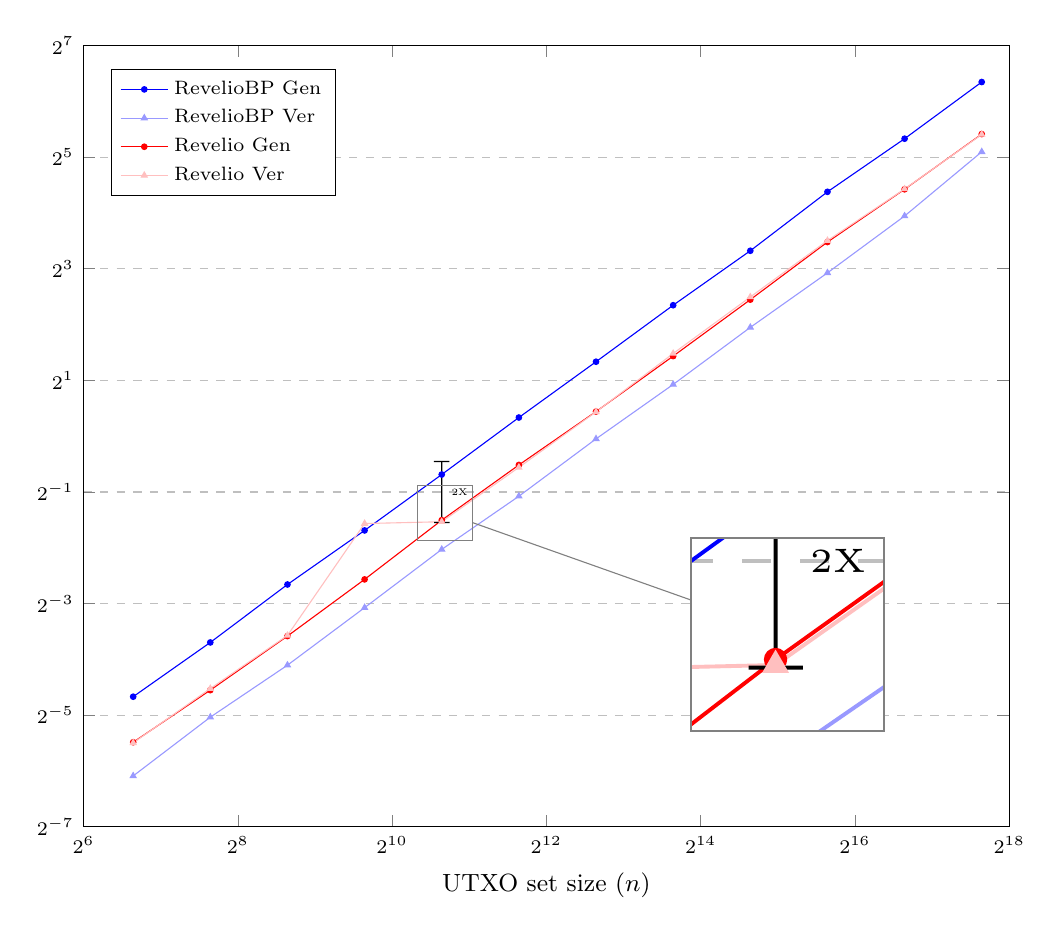
\begin{tikzpicture}[spy using outlines=
      {rectangle, magnification=3.5, size=1cm, connect spies}]
      \begin{axis}[
        width = 1.1\textwidth,
          % title={(b) Running times in min, $s=20$ (log-log)},
          legend cell align={left},
          % title style={font=\scriptsize},
          xlabel style={font=\small},
          ylabel style={font=\tiny},
          legend style={font=\scriptsize},
          xticklabel style={font=\scriptsize},
          yticklabel style={font=\scriptsize},
          xlabel = {UTXO set size ($n$)},
          % ylabel = {Time (in sec)},
          xmin=2^6, xmax=2^18,
          ymin=0.0078125, ymax=128,
          ymode = log,
          log basis y={2},
          xmode = log,
          log basis x={2},
          xtick={64,256,1024, 4096, 16384, 65536, 262144},
          ytick={0.0078125, 0.03125, 0.125, 0.5, 2, 8, 32, 128},
          legend pos=north west,
          % legend style={nodes={scale=0.85, transform shape}},
          ymajorgrids=true,
          grid style=dashed,
      ]
      \addplot+[
          color=Blue,
          mark=*,
          mark options={scale=0.5},
          ]
          coordinates {
          % Updated
          (	100	,	0.03933333333	)
          (	200	,	0.07716666667	)
          (	400	,	0.1585	)
          (	800	,	0.3101666667	)
          (	1600	,	0.6211666667	)
          (	3200	,	1.260833333	)
          (	6400	,	2.5205	)
          (	12800	,	5.0865	)
          (	25600	,	10.00316667	)
          (	51200	,	20.8	)
          (	102400	,	40.23966667	)
          (	204800	,	81.35533333	)
          };
      \addplot+[
          color=lightblue,
          mark=triangle*,
          mark options={scale=0.6},
          ]
          coordinates {
          % Updated
          (	100	,	0.0147	)
          (	200	,	0.0305	)
          (	400	,	0.05816666667	)
          (	800	,	0.1188333333	)
          (	1600	,	0.245	)
          (	3200	,	0.4743333333	)
          (	6400	,	0.967	)
          (	12800	,	1.901333333	)
          (	25600	,	3.861666667	)
          (	51200	,	7.602833333	)
          (	102400	,	15.40383333	)
          (	204800	,	34.184	)
          };
      \addplot+[
          color=red,
          mark=*,
          mark options={scale=0.5},
          ]
          coordinates {
          % Updated
          (	100	,	0.02233333333	)
          (	200	,	0.04266666667	)
          (	400	,	0.0835	)
          (	800	,	0.1688333333	)
          (	1600	,	0.3523333333	)
          (	3200	,	0.6995	)
          (	6400	,	1.357333333	)
          (	12800	,	2.703	)
          (	25600	,	5.45	)
          (	51200	,	11.14716667	)
          (	102400	,	21.46366667	)
          (	204800	,	42.61066667	)
          };
      \addplot+[
          color=pink,
          mark=triangle*,
          mark options={scale=0.6},
          ]
          coordinates {
          % Updated
          (	100	,	0.02216666667	)
          (	200	,	0.0435	)
          (	400	,	0.08416666667	)
          (	800	,	0.3378333333	)
          (	1600	,	0.3455	)
          (	3200	,	0.679	)
          (	6400	,	1.352166667	)
          (	12800	,	2.792	)
          (	25600	,	5.632833333	)
          (	51200	,	11.35083333	)
          (	102400	,	21.53816667	)
          (	204800	,	42.3995	)
          };
    
          \coordinate (spypoint) at (axis cs:1650, 0.3855);
          \coordinate (magnifyglass) at (axis cs:35768,0.0855);
    
          \node[anchor=north] (source) at (axis cs:1600.5,0.34){};
          \node (destination) at (axis cs:1600,0.83){};
          \draw[|-|](source)-- node[anchor=west]{ \scalebox{.7}{\tiny $2$X}} (destination);

          \legend{{\fontfamily{qag}\selectfont RevelioBP} Gen, {\fontfamily{qag}\selectfont RevelioBP} Ver, {\fontfamily{qag}\selectfont Revelio} Gen, {\fontfamily{qag}\selectfont Revelio} Ver}
          \end{axis}
    
        \spy [gray, size=2.45cm] on (spypoint)
              in node[fill=white] at (magnifyglass);
          
    \end{tikzpicture}
  \end{subfigure}
  \hfill
  \begin{subfigure}[b]{0.49\textwidth}
    \caption{\small Running times in min, $n=10^3$}
    \label{subfig:revBP4}
    \tikzexternaldisable
    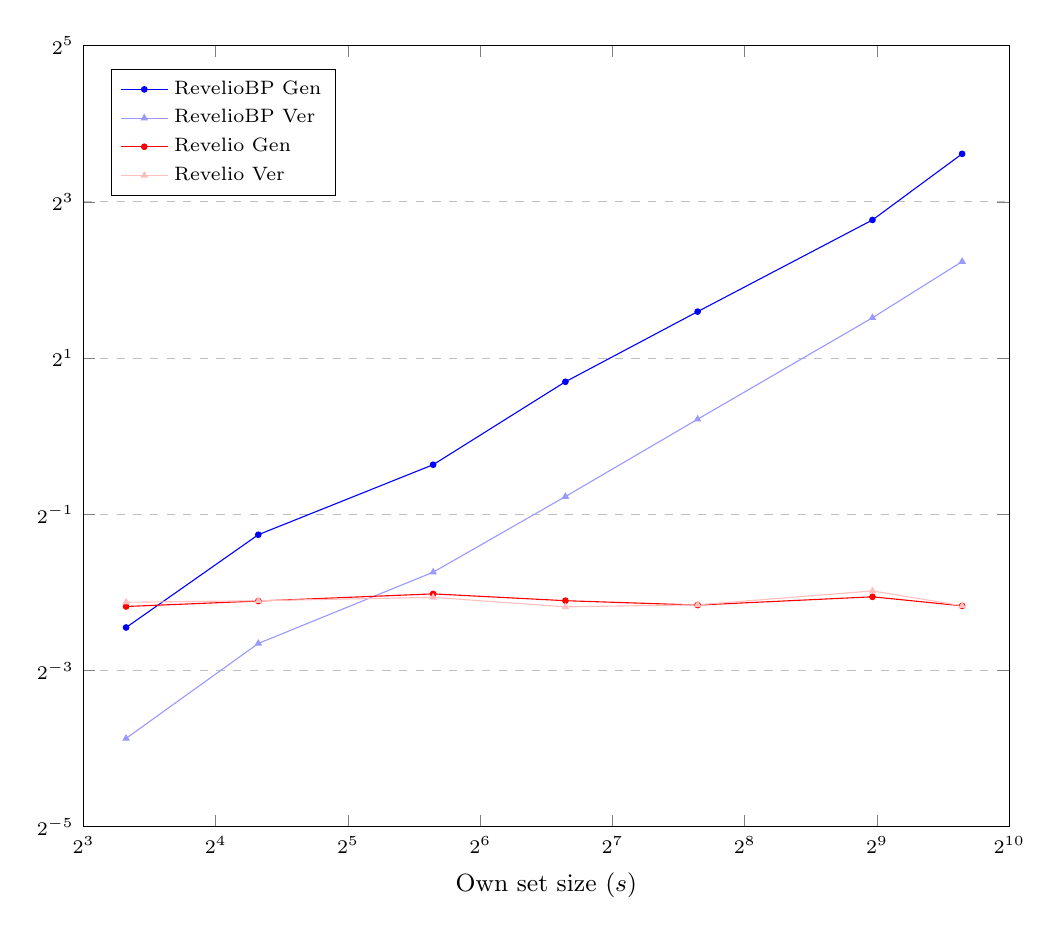
\begin{tikzpicture}
      \begin{axis}[
          width = 1.1\textwidth,
          % title={(c) Running times in min, $n=10^3$ (log-log)},
          legend cell align={left},
          % title style={font=\scriptsize},
          xlabel style={font=\small},
          ylabel style={font=\tiny},
          legend style={font=\scriptsize},
          xticklabel style={font=\scriptsize},
          yticklabel style={font=\scriptsize},
          xlabel = {Own set size ($s$)},
          % ylabel = {Time (in sec)},
          xmin=2^3, xmax=2^10,
          ymin=0.03125, ymax=32,
          ymode = log,
          log basis y={2},
          xmode = log,
          log basis x={2},
          xtick={8, 16,32,64,128,256,512,1024},
          % xtick={8, 32,128,512},
          ytick={0.03125, 0.125, 0.5, 2, 8, 32},
          legend pos=north west,
          % legend style={nodes={scale=0.85, transform shape}},
          ymajorgrids=true,
          grid style=dashed,
      ]
      
      
      \addplot+[
          color=Blue,
          mark=*,
          mark options={scale=0.5},
          ]
          coordinates {
          % Updated
          (	10	,	0.1831666667	)
          (	20	,	0.4171666667	)
          (	50	,	0.7763333333	)
          (	100	,	1.6205	)
          (	200	,	3.019	)
          (	500	,	6.8085	)
          (	800	,	12.24266667	)
          };
      \addplot+[
          color=lightblue,
          mark=triangle*,
          mark options={scale=0.6},
          ]
          coordinates {
          % Updated
          (	10	,	0.0685	)
          (	20	,	0.159	)
          (	50	,	0.2991666667	)
          (	100	,	0.5851666667	)
          (	200	,	1.162166667	)
          (	500	,	2.859166667	)
          (	800	,	4.707	)
          };
      \addplot+[
          color=red,
          mark=*,
          mark options={scale=0.5},
          ]
          coordinates {
          % Updated
          (	10	,	0.2206666667	)
          (	20	,	0.2316666667	)
          (	50	,	0.2468333333	)
          (	100	,	0.2323333333	)
          (	200	,	0.2235	)
          (	500	,	0.2405	)
          (	800	,	0.222	)
          };
      \addplot+[
          color=pink,
          mark=triangle*,
          mark options={scale=0.6},
          ]
          coordinates {
          % Updated
          (	10	,	0.2291666667	)
          (	20	,	0.2323333333	)
          (	50	,	0.2393333333	)
          (	100	,	0.22	)
          (	200	,	0.224	)
          (	500	,	0.2533333333	)
          (	800	,	0.2221666667	)
          };
        \legend{{\fontfamily{qag}\selectfont RevelioBP} Gen, {\fontfamily{qag}\selectfont RevelioBP} Ver, {\fontfamily{qag}\selectfont Revelio} Gen, {\fontfamily{qag}\selectfont Revelio} Ver}
      \end{axis}
    \end{tikzpicture}
  \end{subfigure}
  \caption{Performance comparison of \RB and \R for $\G =$ \texttt{secp256k1} elliptic curve. All the plots are in log-log scale.}
  \label{fig:revBP_plots}
\end{figure}
  
  We have implemented \RPlus in Rust over the secp256k1 elliptic curve. The \R running times were estimated using the simulation code made available by Dutta \textit{et al} \cite{RevelioPerfRepo}.
  All the experiments were run on an Intel Core i7 2.6 GHz CPU.
  Our simulation code is open-sourced on GitHub \cite{RevelioBPPerfRepo}. 
  Figure \ref{subfig:revBP3} shows the \RPlus and \R proof generation and verification times as a function of the UTXO set size for $s=20$.
  % For a constant $s$, we see a linear growth in the timings of both \RB and \R as a function of UTXO set size $n$.
  % The plot shows that the proof generation of \RB is typically 2X slower than that of \Rw.
  % This difference in proof generation timings widens as $s$ increases. 
  % On the other hand, the verification of a \RB proof is much faster than its generation because of a single multi-exponentiation check in the inner product argument verification.
  % In fact, we see that the verification of \RB proof is faster than the verification of a \R proof.
  For a constant own set size $s=10$, we observe the following:
  \begin{enumerate}
    \item[(i)] A linear growth in the running times of both \RB and \R as a function of $n$.
    \item[(ii)] The \RB proof generation is typically 2X slower than that of \R proof generation.
    \item[(iii)] Although both the generation and verification of \RB proofs if linear in $n$ for a constant $s$, the verification is around 2.5X faster than its generation because of a single multi-exponentiation check in the verification of inner product protocol.
    \item[(iv)] The \RB verification is $20\%$ faster than the verification of a \R proof.
  \end{enumerate}
  
  % Another difference between \R and \RB is the dependence of proof generation and verification times on $s$. 
  Furthermore, while the running time of \R is independent of $s$, it scales as $\mathcal{O}(s n)$ for \RBw. 
  % This exacerbates the already high proof generation and verification time of \RB.
  Figure \ref{subfig:revBP4} shows the generation and verification times respectively as a function of $s$ for $n=10^3$.  
  Also, the proof size of \RB proofs grow linearly with $s$ while that of \R remains constant.
  This is shown in Figure \ref{subfig:revBP2} for a constant anonymity set size $n=10^3$.
  This implies that for a constant UTXO set $n$, the verification in \RB is faster than \R only upto a particular $s$.
  Similarly, the difference between \RB and \R proof generation widens as $s$ increases.
  To illustrate this in practical terms, the size of the current UTXO set in the Grin blockchain as of June 7, 2020 is 161,000 \cite{GrinScanWebsite}.
  For this UTXO set size and own output set size equal to 100, an exchange could take upto 160 minutes to generate a \RPlus proof while taking less than $34$ minutes to generate a \R proof.
  The customers of the exchange can verify \RB and \R proofs in 68 and 34 minutes respectively.
  For an exchange which owns 200 outputs in the current UTXO set, the \RB generation and verification times would rise to 320 minutes and 130 minutes respectively, while the timings of \R remain unchanged.
  % Although \RPlus proofs are much slower to generate, they are also much smaller in size. In situations where an exchange may need to store several historical proofs for audit purposes, proof size will be a bigger factor than generation time. Also, these generation times are based on unoptimized non-parallel code on commodity hardware. They can be decreased significantly using multicore CPUs or FPGAs.
  
  % The magnificently smaller size of \RPlus proofs would enable exchanges to store several historical proofs for audit purposes. But the smaller proof size comes at the cost of slow proof generation and verification $(\mathcal{O}(s \cdot n))$.
  % Although the generation times stated above are based on unoptimized non-parallel code on commodity hardware, the proof generation and verification would still be a bottleneck in practical deployment even after a $2\text{ to }3$ times speedup using multi-core CPUs or FPGAs.
  % The verification can significantly be reduced using multi-exponentiation, but prover computation would still be linear in $n$.
  % While ideal in terms of privacy guarantees, \RPlus faces the practical difficulty of slow generation. To this end, we devise an improved \RPlus protocol with similar privacy guarantees, comparable proof size and significantly lower prover and verifier computation. 
  
  \subsection{Scalability and Performance Trade-off}
  
  The smaller proof sizes of \RB would enable exchanges to store several historical proofs for audit purposes.
  Further, if proofs of reserves are to be uploaded on the blockchain for public verifiability, smaller proof size becomes crucial.
  The benefits in scalability due to \RB comes at the price of performance.
  % The verification time can significantly be reduced using multi-exponentiation, but prover computation would still be linear in $sn$. So, if an exchange chooses for smaller proof size, it has to suffer from large generation time.
  From the customer point of view too, larger verification times are undesirable given their limited computational resources.
  %even after multi-exponentiation in verification, more than an hour to verify a proof might be too tedious. 
  
  The simpler formulation of \Rw, on the other hand, allows faster generation and verification. 
  Therefore, if the proof size is not a concern for an exchange, using \R can reduce computational cost for the exchanges as well as the customers. 
  % and feasible to deploy in real-life systems. 
  Moreover, the design of \R allows parallelization of its proof generation as well as verification.
  On the contrary, \RB relies on the recursive inner product protocol, preventing parallelization of proof generation.
  Also, since the base vector used in \RB depends on the tag vector published by an exchange, \RB proofs of multiple exchanges on the same blockchain state cannot be aggregated.  
  Lastly, if exchanges are required to generate proofs of reserves after every $K$ blocks are mined, the proof generation time needs to be less than $K$ minutes\footnote{The average inter-block time is one minute in both Grin and Beam (the two most popular MimbleWimble-based cryptocurrencies).}.
  In such cases, proofs with smaller running times would be preferred.
  
  % The language of \R as well as \RB protocols is based on proving the ownership of $s\text{-out-of-}n$ outputs from an anonymity set.
  % This ensures the privacy of exchange-owned outputs in \R and \RB protocols. 
  % % The exchanges have flexibility in the choice of anonymity set in case of \Rw, while for \RBw, the entire UTXO set corresponding to a particular blockchain state forms the anonymity set.
  % % A \RB proof given by an exchange is implicitly linked to a blockchain state, which implies that  
  % However, in \RBw, the number of exchange-owned outputs is revealed. Since amounts in Grin are in a range of $[0,2^{64})$, one can estimate the maximum reserves an exchange owns knowing 
  % the number of outputs it owns. An adversary who is involved in a transaction with the exchange as a receiver of funds might figure out a lower bound on the reserves. Thus, the exchanges would
  % be skeptical of using \RB since they might not want to reveal the total number of outputs they own. \R does not possess this shortcoming and no information about the reserves is leaked in \Rw.
  
  
  \section{Conclusion}
  To avoid proof sizes which are linear in the size of anonymity set, we have presented Bulletproofs-based proof of reserves protocol \RB with proof size scaling logarithmically in the size of the anonymity set.
  Having implemented \RBw, we conclude that the smaller proof sizes it offers comes with the cost of larger proof generation and verification times.
  \Rw, the first proof of reserves for MimbleWimble, does better in terms of generation and verification times.
  An exchange has to make a trade-off between scalability and performance and choose which protocol suits their needs better: \RB with smaller proof size and large generation times or \R with larger proof sizes and faster generation times. 
  
  
  \section*{Acknowledgements}
  We would like to thank the anonymous reviewers for their insightful comments which helped improve this paper.
  We also acknowledge the support of the Bharti Centre for Communication at IIT Bombay. 
  We thank Piyush Bagad (Wadhwani AI) for help with running the simulations.
  
  % \section{Improved \RPlus}
  
  % % The \proto argument of knowledge individually proves knowledge of each exchange-owned output in the UTXO set $\C_{\text{utxo}}^t$, via a single Bulletproofs-like protocol. 
  % % The prover and verifier computation is $\mathcal{O}(n \cdot s)$ for \protow. Since the size of the UTXO set $(n)$, in general is large, the prover and verifier computation 
  % % becomes a bottleneck for implementing \RPlus in practice. Although the verification can significantly be reduced using multi-exponentiation, prover computation would still be $\mathcal{O}(n \cdot s)$.
  
  % Since \proto reveals the number of exchange-onwed outputs $(s)$, one can guess an exchange-owned output with probability $(\frac{s}{n})$ from the UTXO set.
  % If we consider some different anonymity set structure such that the probability of a random guess of an exchange-owned output remains consistent, we could reduce the prover computation depending on the size of the
  % anonymity set. 
  % % We explore one such structure where each exchange-owned output is assigned a different anonymity set.
  
  % The \proto argument of knowledge individually proves knowledge of each exchange-owned output in the UTXO set $\C_{\text{utxo}}^t$, via a single Bulletproofs-like protocol.
  % Instead of proving that a particular output is one of the outputs in $\C_{\text{utxo}}^t$, we can use a smaller anonymity set for the same. Further, for each output, we could 
  % use a different anonymity set (of same size). Using this idea, we construct an argument of knowledge \Iproto having different anonymity sets for each exchange-owned outputs.
  
  % Consider a set $\textsl{Idx} = \{(b_1, l_1), (b_2, l_2), \dots, (b_s, l_s) \}$ of pair of indices where each $b_j, l_j \in [n]$ denote the beginning and end index respectively of the anonymity set $\textbf{R}_j$ corresponding to exchange-owned output $C_{i_j}$. 
  % Assume that the anonymity set sizes are the same for all $j \in [s]$. Thus, let $n^{\prime} = n_j = (l_j-b_j)$ for all $j \in [s]$.
  % \begin{equation*}
  %   \C_{\text{utxo}}^t = \{ C_1, \ \dots, \ \underbrace{C_{b_j}, \ \dots , \ C_{i_j}, \ \dots, \ C_{l_j}}_{\textbf{R}_j} , \ \dots, \ C_n \}
  % \end{equation*}
  % Note that the set $\textbf{R}_j$ may contain exchange-owned outputs other than $C_{i_j}$. Corresponding to each of these anonymity sets, 
  % we define a binary vector $\textbf{e}_{i_j} \in \{0,1\}^{n^{\prime}}$ such that it has $1$ at index $(i_j - b_j)$ and $0$ otherwise.
  
  % We now design the argument of knowledge \Iproto based on different anonymity sets. The language \Ilang for \Iproto is given as 
  % \begin{align}
  %   \hspace{-1.5mm}
  %   \mathcal{L}_{\RBmath}^I  & = \hspace{-1mm}
  %   \left\{ ( \{\textbf{R}_j\}_{1}^{s}, \textbf{I}) \Bigg| 
  %   \hspace{-3mm}
  %   \text{
  %   \begin{tabular}{c} 
  %   $\exists (\textbf{r}, \textbf{e}_{i_1},\ldots,\textbf{e}_{i_s}) \text{ such that }$
  %   \\ 
  %   $ g^{-r_j} \textbf{R}_j^{\textbf{e}_{j}} = g_t^{-r_j}I_j  \forall j \in [s]$ 
  %   \end{tabular}
  %   }
  %   \hspace{-3mm}
  %   \right\}
  %   \label{eqnRevelioPlus2Language}
  % \end{align} 
  
  % Using a uniformly generated scalar $u \rgen \Z_q$, we combine the constraint equations.
  % \begin{gather}
  %   \prod_{j=1}^{s} \big( g^{-r_j} g_t^{r_j} \textbf{R}_j^{\textbf{e}_{j}}I_j^{-1}\big)^{u^{j-1}} = 1 \nonumber \\
  %   \therefore g^{\eta_1} \cdot g_t^{\eta_2} \cdot \textbf{R}^{\hat{\textbf{e}}} \cdot \hat{I} = 1 \label{mainEquality2}
  % \end{gather}
  
  % \noindent where $\eta_1 = -\langle \textbf{u}^s, \textbf{r} \rangle$, $\eta_2 = -\eta_1$, $\hat{I} = \textbf{I}^{-\textbf{u}^s}$,
  % $\tilde{\textbf{e}} = (\textbf{e}_{i_1} \| u \textbf{e}_{i_2} \| \dots \| u^{s-1} \textbf{e}_{i_s} )$, and
  % $\textbf{R} = (\textbf{R}_1 \| \textbf{R}_2 \| \dots \| \textbf{R}_s)$. Equation (\ref{mainEquality2}) is the \textit{main equality} for \Iproto.
  % For a scalar $w \in \Z_q$ and $\textbf{p} \rgen \G^{(sn^{\prime} + 3)}$
  % and $\textbf{g}^{\prime} \rgen \G^{(sn^{\prime} + s)}$, we construct the base  and exponent (secret) vector as 
  % \begin{align}
  %   \textbf{g}_w &= \big((g \| g_t \| \textbf{R} \| \hat{I})^{\circ w} \circ \textbf{p}\big)  \| \textbf{g}^{\prime} & \in \G^{N} \label{label:Igenerator}\\
  %   \textbf{c}_L &= (\eta_1 \| \eta_2 \| \hat{\textbf{e}} \| 1 \| \Emat \| \textbf{r}) & \in \Z_q^{N}
  % \end{align}
  
  % \noindent where $\Emat = (\textbf{e}_{i_1} \| \dots \| \textbf{e}_{i_s})$ and $N = 2sn^{\prime} + s +3$. 
  
  % %%%%%%%%%%%%%%%%%%
  % % Witness and constraints
  % %%%%%%%%%%%%%%%%%%
  % \begin{center}
  %   \begin{align*}
  %       \textbf{c}_{L} 
  %       &\coloneqq 
  %       (\hspace{1mm}\eta\hspace{1mm} \|
  %       \hspace{1mm}\eta^{\prime}\hspace{1mm}\|
  %       \hspace{6mm} \tilde{\textbf{e}} \hspace{6mm}  \|
  %       \hspace{1.4mm}1 \hspace{1.4mm} \|
  %       \hspace{7mm}
  %       \Emat
  %       \hspace{7mm} \|
  %       \hspace{2.6mm}\textbf{r}\hspace{2.6mm}) \\
  %       \textbf{c}_{R} &\coloneqq (
  %       \hspace{12mm} 
  %       \vecnb{0}^{{n}^{\prime}+3} 
  %       \hspace{12mm} \| 
  %       \hspace{1.65mm}
  %       \Emat - \vecnb{1}^{s {n}^{\prime}}
  %       \hspace{1.65mm}\|
  %       \hspace{1.8mm}
  %       \vecnb{0}^{s}
  %       \hspace{1.8mm})\\[-2pt]
  %       \intertext{\begin{center}
  %           \labelText{\textbf{Fig. 6.} Honest encoding of witness.}{label:witness_2}
  %       \end{center}}\vspace{-1pt}
  %       %%%%%%%%%%%%%%%%%%%%%%%%%%%%%%%
  %       %%%%%%%%%%%%%%%%%%%%%%%%%%%%%%%
  %       \begin{bmatrix}
  %       \textbf{v}_0 \\
  %       \textbf{v}_1 \\
  %       \textbf{v}_2 \\
  %       \textbf{v}_3 \\
  %       \textbf{v}_4 \\
  %       \textbf{v}_5
  %       \end{bmatrix}
  %       &\coloneqq
  %       \setcounter{MaxMatrixCols}{40}
  %       \begin{bmatrix}
  %           \hspace{0.6mm} v & 
  %           \hspace{0.1mm} v & 
  %           \hspace{-1mm} v & 
  %           \hspace{-0.4mm} v & 
  %           \hspace{0.5mm} \vecnb{y}^{sn^{\prime}} & 
  %           \hspace{0.5mm} v \\
  %           \hspace{0.6mm} 1 & 
  %           \hspace{0.1mm} \cdot & 
  %           \hspace{-1mm} \cdot & 
  %           \hspace{-0.4mm} \cdot & 
  %           \hspace{0.5mm} \cdot & 
  %           \hspace{0.5mm} -\vecnb{u}^s \\
  %           \hspace{0.6mm} \cdot & 
  %           \hspace{0.1mm} 1 & 
  %           \hspace{-1mm} \cdot & 
  %           \hspace{-0.4mm} \cdot & 
  %           \hspace{0.5mm} \cdot & 
  %           \hspace{0.5mm} \vecnb{u}^s \\
  %           \hspace{0.6mm} \cdot & 
  %           \hspace{0.1mm} \cdot & 
  %           \hspace{-1mm} \vecnb{1}^{s} \otimes \vecnb{y}^{n^{\prime}} & 
  %           \hspace{-0.4mm} \cdot &
  %           \hspace{0.5mm} \vecnb{u}^s \otimes \vecnb{y}^{n^{\prime}} & 
  %           \hspace{0.5mm} \cdot \\
  %           \hspace{0.6mm} \cdot & 
  %           \hspace{0.1mm} \cdot & 
  %           \hspace{-1mm} \cdot & 
  %           \hspace{-0.4mm} y^s &
  %           \hspace{0.5mm} \vecnb{y}^s \otimes \textbf{1}^{n^{\prime}} & 
  %           \hspace{0.5mm} \cdot \\
  %           \hspace{0.6mm} \cdot & 
  %           \hspace{0.1mm} \cdot & 
  %           \hspace{-1mm} \cdot & 
  %           \hspace{-0.4mm} \cdot &
  %           \hspace{0.5mm} \vecnb{y}^{sn^{\prime}} & 
  %           \hspace{0.5mm} \cdot \\[3pt]
  %       \end{bmatrix}
  %   \end{align*}
  %       \labelText{\textbf{Fig. 7.} Definitions of constraint vectors (Dots mean zero vectors and $v \rgen \Z_q\setminus \{0\}$).}{label:conVec1_2}
  % \end{center}
  
  % The \Iproto protocol can be realised by running \proto described in Protocol (\ref{label:proto1}) with the base vector $\textbf{g}_w$ (equation (\ref{label:Igenerator})), exponent vectors $\textbf{c}_L, \textbf{c}_R$ (Fig. \hyperref[label:witness_2]{6}) and constraint vectors defined by Fig. (\hyperref[label:conVec1_2]{7}).  
  % % Note that the set \textsl{Idx} (which is $\mathcal{O}(s)$) is also published as a part of \Iproto protocol.
  
  % \begin{theorem}
  %   \labelText{}{label:thmImprovedRev+}
  %   Assuming the discrete logarithm assumption holds over $\G$, \Iproto is public-coin, constant-round, perfectly complete,
  %   perfect special honest-verifier zero-knowledge and has computational witness-extended-emulation for extracting a valid $\text{\textsl{wit}}$.
  % \end{theorem}
  % \noindent \textit{Proof}: The proofs for \Iproto follow very closely the proofs of \proto and hence are omitted.
  
  % \subsection{Comparison: \Iproto vs \proto}
  % \label{subscnComparisonIRvsR}
  
  % %TODO Need to argue about privacy guarantee differences between Revelio+ and improved Revelio+
  % For an adversary $\mathcal{A}$ trying to guess index $i_j$ of an exchnage-owned output, we need the probability of guessing randomly from $\textbf{C}$ and $\textbf{R}_j$ to be equal.
  % Let $k \in [n]$ be the index guessed by $\mathcal{A}$. We need  
  % \begin{equation*}
  %   \Pr[ k = i_j | k \leftarrow \mathcal{A}(\textbf{C})] = \Pr[ k = i_j | k \leftarrow \mathcal{A}(\textbf{R}_j)]
  % \end{equation*}
  % Further, since anonymity sets $\textbf{R}_i$ and $\textbf{R}_j$, for some $i, j \in [s]$, could have common outputs, it effectively improves the chances of adversary $\mathcal{A}$ succeeding.
  % Thus, we choose $n^{\prime}$ such that $\frac{1}{n^{\prime} - m} = \frac{s}{n}$, where $m = \textsl{max}_{i,j}\{|\textbf{R}_i \cap \textbf{R}_j|\}$.
  % Assuming $m \ll n^{\prime}$, we have $n^{\prime} \approx \frac{n}{s}$. This implies that the prover as well as verifier computation would be reduced 
  % by a factor of $\frac{s}{2}$ as compared to that in \proto.
  
  % The improved \RPlus protocol has to include the index set \textsl{Idx} in its proof, increasing the proof size by $s$ scalars.
  % The total proof size then becomes $\mathcal{O}(2s + \text{log}_2(2s n^{\prime}))$. For $n^{\prime} \approx \frac{n}{s}$, the proof size of \Iproto is marginally greater than that of \proto.  
  
  % % The analysis of privacy of outputs given multiple \Iproto proofs for different block heights becomes difficult since choice of anonymity sets is left to the prover. 
  % % More precisely, let the anonymity set corresponding to an exchange-owned output $C_{i_j} \in \C_{\text{utxo}}^{t_1} \cap \C_{\text{utxo}}^{t_2}$ be $\textbf{R}_j^1$
  % % and $\textbf{R}_j^2$ respectively for block heights $t_1, t_2$. An adversary can figure out the outputs which remained unchanged comparing $\textbf{R}_j^1$ and $\textbf{R}_j^2$.
  % % This enhances his chances of correctly guessing $i_j$.  
  
  % % If an exchange owns $5\%$ outputs of the UTXO set, the anonymity set
  % % size using \Iproto reduces by $\approx \hspace{-1mm} 20$ times, thus reducing prover and verifier work by $\approx \hspace{-1mm} 10$ times. 
  
  
  % % The proof size in a \Iproto protocol becomes $\mathcal{O}(\text{log}_2(2sn^{\prime} + 2s + 3))$.
  
  
%   \appendices
  %%%%%%%%%%%%%%%%%%%%%%%%%%%
  % Theorem Proofs
  %%%%%%%%%%%%%%%%%%%%%%%%%%%
  \section{Appendix}
  % We present the complete security analysis of the argument of knowledge \proto protocol in the following sections.
  % Although the soundness and zero-knowledge proofs for \proto have some similarities to the security proofs of the ring signature construction in Omniring \cite{Lai2019}, 
  % they are not trivial and necessary to describe the \RPlus protocol completely.
  
  %\subsection{Proof of Lemma \ref{thmNoDLBase}}
  %\label{proofThmNoDLBase}
  %Since $\textbf{g}_w = (\textbf{g}_w^{\prime} \| \textbf{g}^{\prime})$ and $\textbf{g}^{\prime}$ is generated uniformly, we need only to prove that there is no non-trivial discrete logarithm relation between elements of $\textbf{g}_w^{\prime}$. We show that it is difficult to find $\textbf{l}, \textbf{l}^{\prime} \in \Z^{n+3}$ such that 
  %$(\textbf{g}_w^{\prime})^{\textbf{l}} = (\textbf{g}_w^{\prime})^{\textbf{l}^{\prime}}$.
  %Let us denote $\textbf{p} = (p_1, p_2, \dots, p_{n+3})$, $\textbf{l} = (l_1, l_2, \dots, l_{n+3})$ and $\textbf{l}^{\prime} = (l_1^{\prime}, l_2^{\prime}, \dots, l_{n+3}^{\prime})$.
  %
  %Further, suppose the simulator is given a discrete log problem query $(g_0, X)$ where it wants to compute the discrete log of $X$ with respect to $g_0$. 
  %The simulator picks randomly scalars $\lambda_i, \rho_1, \rho_2 \rgen \Z_q $ for all $i \in [n+3]$ and sets $g = g_0, h = g^{\rho_1}, g_t = g^{\rho_2}, \text{ and } p_i = X^{\lambda_i}$.
  %Thus, by definition $C_i = g^{r_i} h^{a_i} = g_0^{(r_i + \rho_1 a_i)}, \text{ and } I_j = g_t^{r_j} h^{a_j} = g_0^{(\rho_2 r_j + a_j)}$.
  %\begin{align*}
  %  (\textbf{g}_w^{\prime})^{\textbf{l}} &= ((g\|g_t\|\textbf{C}\|I_j^{-u})^w \circ \textbf{p})^{\textbf{l}}\\
  %  % &= (g^w p_1 \|g_t^w p_2 \| C_1^w p_3 \| \dots \| C_n^w p_{n+2} \|I_j^{-uw} p_{n+3} )^{\textbf{l}}\\
  %  % &= (g^w p_1)^{l_1} (g_t^w p_2)^{l_2} \prod_{i=3}^{n+2} (C_{i-2}^w p_{i})^{l_{i}} (I_j^{-uw} p_{n+3})^{l_{n+3}}\\
  %  &= g^{w l_1} g_t^{w l_2} I_j^{-uwl_{n+3}} \prod_{i=1}^{n} C_{i}^{w l_{i+2}} \prod_{i=1}^{n+3} p_i^{l_i}
  %  % &= g_0^{w(l_1 + l_2 \rho_2 - u(\rho_2 r_j + a_j)l_{n+3} + \sum_{i=1}^{n}((r_i + \rho_1 a_i)l_{i+2}) )} \cdot X^{\sum_{i=1}^{3} \lambda_i l_i}\\ 
  %  % & \hspace{4mm} X^{\sum_{i=1}^{3} \lambda_i l_i}
  %\end{align*}
  %\noindent Thus, we can write $(\textbf{g}_w^{\prime})^{\textbf{l}} = (\textbf{g}_w^{\prime})^{\textbf{l}^{\prime}}$ as $(\textbf{g}_w^{\prime})^{(\textbf{l} - \textbf{l}^{\prime})} = 1$. 
  %% \vspace{-7pt}
  %% \begin{align*}
  %%   (\textbf{g}_w^{\prime})^{(\textbf{l} - \textbf{l}^{\prime})} = 1
  %% \end{align*}
  %\begin{multline*}
  %  \therefore g_0^{w((l_1-l_1^{\prime}) + (l_2-l_2^{\prime}) \rho_2 - u(\rho_2 r_j + a_j)(l_{n+3}-l_{n+3}^{\prime}))} \\ 
  %  g_0^{w\sum_{i=1}^{n}((r_i + \rho_1 a_i)(l_{i+2}-l_{i+2}^{\prime})) } \cdot X^{\sum_{i=1}^{3} \lambda_i (l_i-l_i^{\prime})} = 1.
  %\end{multline*}
  %\noindent Since $\textbf{l}, \textbf{l}^{\prime}$ are distinct, $l_i \neq l_i^{\prime}$ for atleast one $i \in [n+3]$, the simulator is 
  %able to find a non-trivial discrete log representation of $1$ with respect to $(g_0, X)$. \hfill{\small \qed}
  % \begin{multline*}
  %   \frac{w}{\sum_{i=1}^{n+3} \lambda_i (l_i-l_i^{\prime})} \cdot \big[ ((l_1-l_1^{\prime}) + (l_2-l_2^{\prime}) \rho_2 \\ \hspace{2cm} - u(\rho_2 r_j + a_j)(l_{n+3}-l_{n+3}^{\prime})) \\ + \sum_{i=1}^{n}((r_i + \rho_1 a_i)(l_{i+2}-l_{i+2}^{\prime})) \big].
  % \end{multline*}
  % \begin{flushright}
  %   \qed
  % \end{flushright}
  
  
  
  \subsection{Proof of Theorem \hyperref[label:thm1]{1} (Perfect SHVZK)}
  \label{scnProofTheorem1}
  \vspace{-2pt}
  Let the verifier challenges be $(u, v, w, y, z, x)$. Simulator $\mathcal{S}$ computes $\hat{I}(u), \textbf{g}_w(u,w)$ as described in \protow. 
  We will use $\delta(u,v,y,z)$ to make the dependence of $\delta$ (as defined in Fig. \ref{fig:conVec2}) on the challenges explicit.
  % \begin{align}
  %     \hat{I} &= \ \textbf{I}^{\vecnb{u}^s},\\
  %     \textbf{g}_w &= \left[((g\|g_t\|\textbf{C}\|\hat{I})^{\circ w} \circ \textbf{p}) \| \textbf{g}^{\prime}\right].
  % \end{align}
  Now, $\mathcal{S}$ samples the following quantities uniformly from respective groups: $S, T_2 \rgen \G, \ \lvec, \rvec \rgen \Z_q^N \ \tau_x, r \rgen \Z_q$.
  It then computes the remaining quantities corresponding to the ones which were sent by $\P$ to $\V$ in \proto as follows:
  \begin{align}
      \hat{t} &= \langle \lvec, \rvec \rangle,\\
      T_1 &= (g^{\hat{t} - \delta} h^{\tau_x} T_2^{-x^2})^{x^{-1}},\\
      A &= (h^{\prime})^r S^{-x} \textbf{g}_w^{\lvec - \vecnb{\alpha}} \textbf{h}^{\vecnb{\theta}^{\circ -1} \circ \rvec - \vecnb{\beta}}. \label{label:a}
  \end{align}
  
  Finally, $\mathcal{S}$ outputs the simulated transcript $(A, S,$ $T_1, T_2, \lvec, \rvec, \hat{t}, \tau_x, r)$. 
  Note that since $\lvec, \rvec$ are uniformly sampled from $\Z_q^N$, $\hat{t}$ is uniformly distributed in $\Z_q$. $T_1$ is also uniformly distributed in $\G$ as $g,h, T_2$ are uniformly sampled from $\G$ and the corresponding exponents are also uniformly distributed in $\Z_q$.
  From Lemma \ref{thmNoDLBase}, recall that $\textbf{g}_w$ can also be considered as uniformly distributed in $\G^{n+3}$. Thus, $A$ is also uniformly distributed in $\G$ since the generators as well as exponents in the equation for computing $A$ are uniformly distributed in the respective groups.
  This implies that all the elements produced by $\mathcal{S}$ and those produced by \proto are identically distributed and also satisfy the verification equations at the end of Figure \ref{fig:protocol_revBP}.
  Therefore, the protocol is perfect special honest-verifier zero knowledge. \hfill{\small \qed}
  % \begin{flushright}
  %   \qed
  % \end{flushright}
  
  
  \subsection{Proof of Theorem \hyperref[label:thm2]{2} (Soundness)}
  \label{scnProofTheorem2}
  \vspace{-3pt}
  To prove that \proto has witness-extended emulation, first we state a couple of useful lemmas and a corollary.
  Before we proceed, we define some notation and a new system of constraint equations \textsf{CS}. Let $\vecnb{\gamma}_L, \vecnb{\gamma}_R \in \Z_q^N$ be
  \begin{align*}
      \vecnb{\gamma}_{L} 
      &\coloneqq 
      (\hspace{0.25mm} \gamma_{L,1} \hspace{0.25mm} \|
      \hspace{0.58mm} \gamma_{L,2} \hspace{0.55mm}\|
      \hspace{0.9mm} \vecnb{\gamma}_{L,3} \hspace{0.9mm}\|
      \hspace{0.6mm} \gamma_{L,4} \hspace{0.6mm}\|
      \hspace{4mm}
      \vecnb{\gamma}_{L,5}
      \hspace{4mm} \|
      \hspace{1mm} \vecnb{\gamma}_{L,6} \hspace{1mm}),\\
      \vecnb{\gamma}_{R} &\coloneqq 
      (\underbrace{\hspace{-0.2mm} \gamma_{R,1} \hspace{-0.2mm}}_{1} \|
      \underbrace{\hspace{-0.2mm} \gamma_{R,2} \hspace{-0.2mm}}_{1}\|
      \underbrace{\hspace{0.1mm} \vecnb{\gamma}_{R,3} \hspace{0.1mm}}_{n}\|
      \underbrace{\hspace{-0.2mm} \gamma_{R,4} \hspace{-0.2mm}}_{1}\|
      \underbrace{\hspace{3.2mm} \vecnb{\gamma}_{R,5} \hspace{3.2mm}}_{sn} \|
      \underbrace{\hspace{0.38mm} \vecnb{\gamma}_{R,6} \hspace{0.38mm}}_{s}),
  \end{align*}
  where for $i \in \{L,R\}$, $\gamma_{i,j} \in \Z_q$ for $j\in \{1,2,4\}$, $\vecnb{\gamma}_{i,3} \in \Z_q^n$, $\vecnb{\gamma}_{i,6} \in \Z_q^s$ and for some matrices $\Upgamma_L, \Upgamma_R \in \Z_q^{s \times n}$, $\vecnb{\gamma}_{i,5} = \textsl{vec}(\Upgamma_{i}) \in \Z_q^{sn}$.
  Define the constraint system \textsf{CS} with parameter $u$ such that $\textsf{CS}(\vecnb{\gamma}_L, \vecnb{\gamma}_R) = 0 \iff$
  % \begin{align*}
  %   \textsf{CS}(\vecnb{\gamma}_L, \vecnb{\gamma}_R) = 0 \iff
  % \end{align*}
  \begin{numcases}{}
          \vecnb{\gamma}_{L,5} \circ \vecnb{\gamma}_{R,5} &= $\ \vecnb{0}^{sn}$, \label{eqn:dotprod_TauL_TauR} \\
          \gamma_{L,1} &= $-\langle \vecnb{u}^s, \vecnb{\gamma}_{L,6} \rangle$,\\
          \gamma_{L,2} &= $\langle \vecnb{u}^s, \vecnb{\gamma}_{L,6} \rangle$,\\
          \vecnb{\gamma}_{L,3} &= $\ \vecnb{u}^s \Upgamma_{L}$,\\
          \Upgamma_{L} \vecnb{1}^{n} &= $\ \vecnb{1}^{s}$, \label{eqn:TauLvec} \\
          \gamma_{L,4} &= $1$,\\
          \vecnb{\gamma}_{L,5} &= $-\vecnb{\gamma}_{R,5} + \vecnb{1}^{sn}$. \label{eqn:rel_TauL_TauR}
  \end{numcases}
  \vspace{-2pt}
  \begin{lemma}\label{lemEQimpliesCS}
    For a fixed $q > 2^{\lambda}$ and $u,v \in \Z_q$, suppose there exist $\vecnb{\gamma}_L, \vecnb{\gamma}_R \ \in \Z_q^N $ such that we have \textsf{EQ}$(\vecnb{\gamma}_L, \vecnb{\gamma}_R)=0$ for $sn$ different values of $y$ and two different values of $v$, then \textsf{CS}$(\vecnb{\gamma}_L, \vecnb{\gamma}_R)=0$.
  \end{lemma}
  \vspace{-2pt}
  \textit{Proof}: Since \textsf{EQ}$(\vecnb{\gamma}_L, \vecnb{\gamma}_R)=0$ for $sn$ different values of $y$, the following polynomials in $y$ of degree at most $sn-1$ have $sn$ different roots. Thus, all of them must be equal to \textit{zero} polynomials.
  \begin{align*}
    \langle \vecnb{\gamma}_{L,5} \circ \vecnb{\gamma}_{R,5}, \vecnb{y}^{sn} \rangle = 0 & & \hspace{1cm} \text{by (\ref{ceq0})},\\
      v\cdot \gamma_{L,1} + \gamma_{L,2} + (v-1) \langle \vecnb{\gamma}_{L,6}, \vecnb{u}^s \rangle = 0 & & \hspace{1cm} \text{by (\ref{ceq1})},\\
      \langle \vecnb{\gamma}_{L,3} - \vecnb{u}^s \Upgamma_L, \vecnb{y}^{n} \rangle = 0 & & \hspace{1cm} \text{by (\ref{ceq2})},\\
      (\gamma_{L,4} -1)y^s  + \langle \Upgamma_L \vecnb{1}^n - \vecnb{1}^s, \vecnb{y}^s \rangle = 0 & & \hspace{1cm} \text{by (\ref{ceq3})},\\
      \langle \vecnb{\gamma}_{L,5} + \vecnb{\gamma}_{R,5} - \vecnb{1}^{sn}, \vecnb{y}^{sn} \rangle = 0 & & \hspace{1cm} \text{by (\ref{ceq4})}.
  \end{align*}
  Furthermore, since \textsf{EQ}$(\vecnb{\gamma}_L, \vecnb{\gamma}_R)=0$ for two different values of $v$ too, the coefficient of $v$ and the constant term in the second equation both must be \textit{zero}.  
  By comparing coefficients, we get $\textsf{CS}(\vecnb{\gamma}_L, \vecnb{\gamma}_R)=0$. \hfill{\small \qed}
  
  \begin{lemma}\label{lemTauLBinary}
    If \textsf{CS}$(\vecnb{\gamma}_L, \vecnb{\gamma}_R) = 0$ then each row of $\Upgamma_L$ is a unit vector of length $n$.
  \end{lemma}
  \textit{Proof}: This follows from equations (\ref{eqn:dotprod_TauL_TauR}), (\ref{eqn:TauLvec}) and (\ref{eqn:rel_TauL_TauR}). \hfill{\small \qed}
  
  \begin{corollary}\label{corollaryNoDL}
    Assuming the discrete logarithm assumption holds over $\G$, a \textsf{PPT} adversary cannot find a non-trivial discrete logarithm relation between the components of the base $(h^{\prime}\|\textbf{g}_w \| \textbf{h})$
  \end{corollary}
  \textit{Proof}: Since $(h^{\prime}, \textbf{h})$ are generated uniformly from $\G$, it is infeasible for a PPT adversary to compute its discrete log relation with base vector $\textbf{g}_w$.
  Proving that a \textsf{PPT} adversary cannot find a non-trivial discrete log relation between components of $\textbf{g}_w$ follows from Lemma \ref{thmNoDLBase}. \hfill{\small \qed}
  
  
  With the above lemmas and the corollary, we proceed to construct an extractor $\E$. 
  Let $\textsl{pp} \leftarrow \textsl{Setup}(\lambda)$ and $\textsl{stmt, wit} \leftarrow \mathcal{A}(\textsl{pp})$.
  The aim of $\E$ is to produce a \textit{valid} transcript and consequently the witness $\textsl{wit}^{\prime}$ corresponding to that transcript.
  Since $\E$ has oracle access to $\langle \P^{\star}(\textsl{pp, stmt; wit}), \V(\textsl{pp, stmt}) \rangle$ for any prover $\P^{\star}$, producing a valid transcript
  is trivial for $\E$. We hence focus on how $\E$ could extract a valid witness. 
  
  Extractor $\E$ runs $\P^{\star}$ on one value each of $u, v$, 2 different values of $w$, $sn$ different values of $y$,
  5 different values of $z$ and 3 different values of $x$. This results in $30\times sn$ transcripts.
  $\E$ fixes the values of $(w,y,z)$ and runs $\P^{\star}$ for $x=(x_1,x_2,x_3)$. Let the transcripts for the respective $x$ be $(A, S, T_1, T_2, \tau_{x_i}, r_{x_i}, \lvec_{x_i}, \rvec_{x_i}, \hat{t}_{x_i})$ for $i=1,2,3$. Now $\E$ will extract the discrete logarithm representations of $A, S, T_1, T_2$ using the above transcripts.\\
  
  \textbf{Extracting $A$}: Choose $k_i \in \Z_q \text{ for } i=1,2$ such that $\sum_{i=1}^{2} k_i =1$ and $\sum_{i=1}^{2} k_ix_i =0$. From (\ref{label:a}), we have
  % \begin{gather*}
  %     A^{k_i} = h^{r_{x_i}k_i} S^{-x k_i} \textbf{g}_w^{k_i \cdot (\lvec_{x_i} - \vecnb{\alpha})} \textbf{h}^{k_i \cdot (\vecnb{\theta}^{\circ -1} \circ \rvec_{x_i} - \vecnb{\beta})} \ \forall i \in \{1,2\}
  % \end{gather*}
  \begin{multline*}
      \prod_{i=1}^{2} A^{k_i} = h^{\sum_{i} r_{x_i}k_i} S^{-\sum_{i} k_i x_i}  
      \textbf{g}_w^{ (\sum_{i} k_i \cdot \lvec_{x_i}) - \vecnb{\alpha}(\sum_{i} k_i)}  \\[-4pt]
      \textbf{h}^{(\sum_{i} k_i \vecnb{\theta}^{\circ -1} \circ \rvec_{x_i}) - \vecnb{\beta}(\sum_{i} k_i)},
  \end{multline*}
  \begin{align*}
      & \implies A = h^{\sum_{i} r_{x_i}k_i} 
      \textbf{g}_w^{(\sum_{i} k_i \cdot \lvec_{x_i}) - \vecnb{\alpha}}
      \textbf{h}^{(\sum_{i} k_i \vecnb{\theta}^{\circ -1} \circ \rvec_{x_i}) - \vecnb{\beta}},\\
      & \implies A = h^{r_A^{\prime}} \textbf{g}_w^{\textbf{c}_L^{\prime}} \textbf{h}^{\textbf{c}_R^{\prime}}.
  \end{align*}
  where $r_A^{\prime} = \sum_{i} r_{x_i}k_i$, $\textbf{c}_L^{\prime} = \left( \sum_{i}  k_i \cdot \lvec_{x_i} \right) - \vecnb{\alpha}$ and $\textbf{c}_R^{\prime} = \left(\sum_{i} k_i \cdot (\vecnb{\theta}^{\circ -1} \circ \rvec_{x_i}) \right) - \vecnb{\beta}$.
  Since we have considered the above extraction for a particular $w$ out of the 2 of its values, $r_A^{\prime}, \textbf{c}_L^{\prime}, \textbf{c}_R^{\prime}$ depend on $w$. 
  To show that the discrete logarithm representation of $A$ is independent of w, $\E$ repeats the above for a different $w^{\prime}$. In particular, we have $A= h^{r_A^{\prime \prime}} \textbf{g}_{w^{\prime}}^{\textbf{c}_L^{\prime \prime}} \textbf{h}^{\textbf{c}_R^{\prime \prime}}$. 
  Now we have two possibly different representations of $A$. Write $\textbf{c}_L^{\prime} = (\textbf{c}_{L,1}^{\prime} \| \textbf{c}_{L,2}^{\prime})$  and $\textbf{c}_L^{\prime \prime} = (\textbf{c}_{L,1}^{\prime \prime} \| \textbf{c}_{L,2}^{\prime \prime})$ of appropriate dimensions. We have
  \begin{gather*}
      h^{r_A^{\prime}} \textbf{g}_w^{\textbf{c}_L^{\prime}} \textbf{h}^{\textbf{c}_R^{\prime}} =
      h^{r_A^{\prime \prime}} \textbf{g}_{w^{\prime}}^{\textbf{c}_L^{\prime \prime}} \textbf{h}^{\textbf{c}_R^{\prime \prime}} \implies \\
      1 = h^{r_A^{\prime} - r_A^{\prime \prime}} 
      (g \| g_t \| \textbf{C} \| \hat{I})^{w \cdot \textbf{c}_{L,1}^{\prime} - w^{\prime} \cdot \textbf{c}_{L,1}^{\prime \prime}} 
      (\textbf{p}\|\textbf{g}^{\prime})^{\textbf{c}_{L}^{\prime} - \textbf{c}_{L}^{\prime \prime}}
      \textbf{h}^{\textbf{c}_{R}^{\prime} - \textbf{c}_{R}^{\prime \prime}}.
  \end{gather*}
  
  Now, if $r_A^{\prime} \neq r_A^{\prime \prime}, \ \textbf{c}_{L}^{\prime} \neq \textbf{c}_{L}^{\prime \prime}, \ \textbf{c}_{R}^{\prime} \neq \textbf{c}_{R}^{\prime \prime}$, since $(\textbf{p}\| \textbf{g}^{\prime} \| \textbf{h})$ is uniformly chosen after fixing $(g \| g_t \| \textbf{C} \| \hat{I})$, 
  we would have violated the discrete logarithm assumption. Thus, $r_A^{\prime} = r_A^{\prime \prime}, \ \textbf{c}_{L}^{\prime} = \textbf{c}_{L}^{\prime \prime}, \ \textbf{c}_{R}^{\prime} = \textbf{c}_{R}^{\prime \prime}$ and letting $\textbf{c}_L^{\prime} = (\xi^{\prime} \| \xi^{\prime \prime} \| \hat{\textbf{e}}^{\prime} \| \psi^{\prime})$,
  we get 
  % \begin{align}
  %     1 &= (g \| g_t \| \textbf{C} \| \hat{I})^{(w-w^{\prime}) \cdot \textbf{c}_L^{\prime}}\nonumber\\
  %     1 &= (g \| g_t \| \textbf{C} \| \hat{I})^{\textbf{c}_L^{\prime}} \text{  since } w \neq w^{\prime}\nonumber\\
  %     1 &= \big(g^{\xi^{\prime}} \cdot g_t^{\xi^{\prime \prime}} \cdot \textbf{C}^{\hat{\textbf{e}}^{\prime}} \cdot \hat{I}^{\psi^{\prime}} \big) \label{label:wit_1}
  % \end{align}
  \begin{gather}
    1 = (g \| g_t \| \textbf{C} \| \hat{I})^{(w-w^{\prime}) \cdot \textbf{c}_L^{\prime}}, \nonumber \\
    \implies \hspace{1.8mm} 1 = (g \| g_t \| \textbf{C} \| \hat{I})^{\textbf{c}_L^{\prime}} \text{  since } w \neq w^{\prime}, \nonumber \\
    \hspace{-14.1mm} \implies \hspace{1.8mm} 1 = g^{\xi^{\prime}} \cdot g_t^{\xi^{\prime \prime}} \cdot \textbf{C}^{\hat{\textbf{e}}^{\prime}} \cdot \hat{I}^{\psi^{\prime}}. \label{label:wit_1}
  \end{gather}
  We will use equation (\ref{label:wit_1}) in the last part of the proof.\\
  
  \textbf{Extracting $S$}: $\E$ samples some $k_1, k_2 \in \Z_q$ such that $\sum_{i}k_i=0$ and $\sum_{i}k_ix_i=1$. From (\ref{label:a}), we have
  % \begin{gather*}
  %     S^{x_i} = h^{r_{x_i}} A^{-1} \textbf{g}_w^{\lvec_{x_i} - \vecnb{\alpha}} \textbf{h}^{\vecnb{\theta}^{\circ -1} \circ \rvec_{x_i} - \vecnb{\beta}} \ \forall i \in \{1,2\}
  % \end{gather*}
  % \begin{multline*}
  %   \prod_{i=1}^{2}S^{k_ix_i} = h^{\sum_i k_ir_{x_i}} 
  %     A^{-\sum_i k_i} 
  %     \textbf{g}_w^{(\sum_i k_i \cdot \lvec_{x_i}) - (\sum_i k_i)\vecnb{\alpha}} \\[-4pt]
  %     \textbf{h}^{( \sum_i k_i \cdot \vecnb{\theta}^{\circ -1} \circ \rvec_{x_i}) - (\sum_i k_i)\vecnb{\beta}}
  % \end{multline*}
  \begin{gather}
    S = h^{r_S^{\prime}} \textbf{g}_w^{\sum_i k_i \cdot \lvec_{x_i}} \textbf{h}^{\sum_i k_i \cdot \vecnb{\theta}^{\circ -1} \circ \rvec_{x_i}} = h^{r_S^{\prime}} \textbf{g}_w^{\textbf{s}_L^{\prime}} \textbf{h}^{\textbf{s}_R^{\prime}}.
    % \therefore S = h^{r_S^{\prime}} \textbf{g}_w^{\textbf{s}_L^{\prime}} \textbf{h}^{\textbf{s}_R^{\prime}} 
  \end{gather}
  
  For a fixed $w$, the extracted $A, S$ hold for all possible $(x,y,z)$ because otherwise, the discrete log assumption would be violated owing to Corollary \ref{corollaryNoDL} as a non-trivial discrete logarithm representation of $1$ with respect to the base $(h^{\prime}\| \textbf{g}_w \| \textbf{h})$ would be known.
  
  Substituting these expressions of $A, S$ in the expressions for $\lvec, \rvec$ from the protocol, we get
  \begin{gather*}
      \lvec_x^{\prime} = \ \textbf{c}_L^{\prime} + \vecnb{\alpha} + \textbf{s}_L^{\prime} \cdot x \ \in \Z_q^N, \\
      \rvec_x^{\prime} = \ \vecnb{\theta} \circ \ (\textbf{c}_R^{\prime} + \textbf{s}_R^{\prime} \cdot x) + \vecnb{\mu} \ \in \Z^N_q.
  \end{gather*}
  
  These vectors must also hold for all $(x,y,z)$ because if that was not the case, then we would know a non-trivial discrete logarithm representation of $1$ with respect to the base $(h^{\prime}\| \textbf{g}_w \| \textbf{h})$ due to Corollary \ref{corollaryNoDL}.\\
  
  
  % \textbf{Extracting $T_1,T_2$}: The verification equation for checking $\hat{t}=t_0+t_1x +t_2x^2$ in the protocol can be rewritten as follows:
  % \begin{gather*}
  %     g^{\hat{t}}h^{\tau_x} \stackrel{?}{=} g^{\delta} T_1^{x} T_2^{x^2}\\
  %     \iff
  %     T_1^{x} \stackrel{?}{=} g^{\hat{t}-\delta} h^{\tau_x} T_2^{-x^2} \quad  \text{or} \quad T_2^{x^2} = g^{\hat{t}-\delta} h^{\tau_x} T_1^{-x}
  % \end{gather*}
  
  \textbf{Extracting $T_1,T_2$}:  $\E$ chooses $k_i \in \Z_q \text{ for } i \in \{1,2,3\}$ such that $\sum_{i=1}^{3}k_i=0$, $\sum_{i=1}^{3}k_ix_i=1$ and $\sum_{i=1}^{3}k_ix_i^2=0$. Thus, we have
  \begin{gather*}
      T_1 = \prod_{i=1}^{3} T_1^{k_ix_i} = g^{\sum_{i=1}^{3} k_i \hat{t}_{x_i}} h^{\sum_{i=1}^{3} k_i \tau_{x_i}} = g^{t_1^{\prime}} h^{r_1^{\prime}}.
      % \implies 
      % T_1 = g^{t_1^{\prime}} h^{r_1^{\prime}}
  \end{gather*}
  
  Similarly, to extract $T_2$, $\E$ chooses $k_i^{\prime} \in \Z_q \text{ for } i \in \{1,2,3\}$ such that $\sum_{i=1}^{3}k_i^{\prime}=0$, $\sum_{i=1}^{3}k_i^{\prime}x_i=0$ and $\sum_{i=1}^{3}k_i^{\prime}x_i^2=1$. Thus, we have
  \begin{gather*}
      T_2 = \prod_{i=1}^{3} T_2^{k_i^{\prime} x_i^2} = g^{\sum_{i=1}^{3} k_i^{\prime} \hat{t}_{x_i}} h^{\sum_{i=1}^{3} k_i^{\prime} \tau_{x_i}} = g^{t_2^{\prime}} h^{r_2^{\prime}}.
      % \implies 
      % T_2 = g^{t_2^{\prime}} h^{r_2^{\prime}}
  \end{gather*}
  
  Again, the above expressions for $T_1, T_2$ hold for all $x$, or otherwise we would have obtained a non-trivial discrete logarithm representation of $1$ base $(g\|h)$ violating the discrete logarithm assumption.
  Therefore, we have obtained $t_1^{\prime}, t_2^{\prime} \in \Z_q$ as the exponents of $g$ in the extracted $T_1$ and $T_2$ respectively.\\
  
  \textbf{Extracting witness}: $\E$ parses $\textbf{c}_L^{\prime}$ as below and outputs the witness $\textsl{wit}^{\prime}$ 
  \begin{align*}
      \textbf{c}_L^{\prime} &= (\xi^{\prime} \| \xi^{\prime \prime} \| \hat{\textbf{e}}^{\prime} \| \psi^{\prime}\| \textsl{vec}(\Emat^{\prime}) \| \textbf{r}^{\prime}), \\
      \textsl{wit}^{\prime} &= (\textbf{r}^{\prime}, \textbf{e}_{i_1}^{\prime}, \dots \textbf{e}_{i_s}^{\prime}).
  \end{align*}
  
  Finally, what remains to show is that the extracted witness is a valid witness to the statement $\textsl{stmt}$. Using the extracted $t_1^{\prime}, t_2^{\prime}$ we have
  \begin{gather*}
      t_{x}^{\prime} = \delta(u,v,y, z) + t_1^{\prime}x + t_2^{\prime}x^2.
  \end{gather*}
  for all $(x,y,z)$ or else we would violate the DL assumption by having a DL relation between $g,h$. Let
  \begin{align*}
      t_0^{\prime} &\coloneqq \delta(u,v,y, z), \\
      l^{\prime}(X) &\coloneqq \ \textbf{c}_L^{\prime} + \vecnb{\alpha} + \textbf{s}_L^{\prime} \cdot X ,
      \\
      r^{\prime}(X) &\coloneqq \ \vecnb{\theta} \circ \ (\textbf{c}_R^{\prime} + \textbf{s}_R^{\prime} \cdot X) + \vecnb{\mu},
      \\
      t^{\prime}(X) &\coloneqq \langle l^{\prime}(X),r^{\prime}(X) \rangle.
  \end{align*}
  Now, the following polynomial, for all $(y,z)$, has at least 3 roots and hence must be a zero polynomial.
  \begin{align*}
      t^{\prime}(X) - (t_0^{\prime} + t_1^{\prime}X + t_2^{\prime}X^2).
  \end{align*}
  We have $t^{\prime}(X) = t_0^{\prime} + t_1^{\prime}X + t_2^{\prime}X^2 $ and particularly, $t^{\prime}(0) = t_0^{\prime}$. The latter two quantities are given by 
  \begin{align}
      t_0^{\prime} &= z^3 \cdot \langle \vecnb{1}^{s+1}, \vecnb{y}^{s+1} \rangle + \langle \vecnb{\alpha}, \vecnb{\mu} \rangle + \langle \vecnb{1}^N, \vecnb{\nu}\rangle, \label{label:t0}\\
      t^{\prime}(0) &= 
      \langle \textbf{c}_L^{\prime}, \vecnb{\theta} \circ \textbf{c}_R^{\prime} \rangle + 
      \langle \textbf{c}_L^{\prime}, \vecnb{\mu} \rangle
      +
      \langle \textbf{c}_R^{\prime}, \vecnb{\theta} \circ \vecnb{\alpha} \rangle
      +
      \langle \vecnb{\alpha}, \vecnb{\mu} \rangle, \nonumber \\[2pt]
      % &=
      % \langle \textbf{c}_L^{\prime}, \vecnb{\theta} \circ \textbf{c}_R^{\prime} \rangle + 
      % \langle \textbf{c}_L^{\prime}, \vecnb{\zeta} \rangle
      % + 
      % \langle \textbf{c}_L^{\prime}, \vecnb{\nu} \rangle
      % +
      % \langle \textbf{c}_R^{\prime}, \vecnb{\nu} \rangle
      % +
      % \langle \vecnb{\alpha}, \vecnb{\mu} \rangle \nonumber\\[2pt]
      &=
      \langle \textbf{c}_L^{\prime}, \vecnb{\theta} \circ \textbf{c}_R^{\prime} \rangle + 
      \langle \textbf{c}_L^{\prime}, \vecnb{\zeta} \rangle \ +
      \nonumber
      \\
      &
      \hspace{2.62cm}
      \langle \textbf{c}_L^{\prime}+\textbf{c}_R^{\prime}, \vecnb{\nu} \rangle
      +
      \langle \vecnb{\alpha}, \vecnb{\mu} \rangle, \label{label:tX0}
  \end{align}
  where $\vecnb{\zeta} = \sum_{i=1}^{3} z^{i} \textbf{v}_i$. Equations (\ref{label:t0}) and (\ref{label:tX0}) imply
  \begin{align*}
      z^3 \langle \vecnb{1}^{s+1}, \vecnb{y}^{s+1} \rangle
      %&= \langle \textbf{c}_L^{\prime}, \vecnb{\theta} \circ \textbf{c}_R^{\prime} \rangle + 
      %\langle \textbf{c}_L^{\prime}, \vecnb{\zeta} \rangle
      %+ \\[2pt]
      %& \hspace{0.5cm}
      %\langle \textbf{c}_L^{\prime}-\textbf{c}_R^{\prime} - \vecnb{1}^{t}, \vecnb{\nu} \rangle
      %+
      %\langle \vecnb{\alpha}, \vecnb{\mu} \rangle
      %\\[2pt]
      &= 
      \langle \textbf{c}_L^{\prime}, \textbf{v}_0 \circ \textbf{c}_R^{\prime} \rangle + 
      \sum_{i=1}^{3} z^i \langle \textbf{c}_L^{\prime}, \textbf{v}_i \rangle
      \\%[2pt]
      & \hspace{0.5cm}
      + 
      z^4 \langle \textbf{c}_L^{\prime}+\textbf{c}_R^{\prime} - \vecnb{1}^{N}, \textbf{v}_4 \rangle.
  \end{align*}
  
  The above equation holds for $5$ different values of $z$. 
  As the equation involves a degree 4 polynomial, the coefficients on both sides must be equal. 
  This implies that $\textsf{EQ}(\textbf{c}_L^{\prime}, \textbf{c}_R^{\prime})=0$ for $sn$ different values of $y$ and $2$ values of $v$. 
  By Lemma \ref{lemEQimpliesCS}, we have $\textsf{CS}(\textbf{c}_L^{\prime}, \textbf{c}_R^{\prime})=0$. 
  Further, Lemma \ref{lemTauLBinary} implies that each row vector of $\Emat^{\prime}$ is a unit vector of length $n$.
  Let $\textsl{vec}(\Emat^{\prime}) = (\textbf{e}_{i_1}^{\prime}, \dots, \textbf{e}_{i_s}^{\prime})$ and write
  \begin{equation*}
      \xi^{\prime} = -\langle \vecnb{u}^s, \textbf{r}^{\prime} \rangle, \ \xi^{\prime \prime} = \langle \vecnb{u}^s, \textbf{r}^{\prime}\rangle, \
      \psi^{\prime} = 1, \
      \hat{\textbf{e}}^{\prime} = \vecnb{v}^{s}\Emat^{\prime}.
  \end{equation*}
  
  Also, let $i_1^{\prime}, i_2^{\prime}, \dots, i_s^{\prime}$ be the indices of the non-zero numbers in vector
  $\hat{\textbf{e}}^{\prime}$. We now show that these exponents computed from the extracted witness
  $(\textbf{r}^{\prime}, \textbf{e}_{i_1}^{\prime}, \textbf{e}_{i_2}^{\prime}, \dots, \textbf{e}_{i_s}^{\prime} )$ is correct.
  From (\ref{label:wit_1}), we have
  \begin{align*}
      1 =& \ g^{\xi^{\prime}} \cdot g_t^{\xi^{\prime \prime}} \cdot \textbf{C}^{\hat{\textbf{e}}^{\prime}} \cdot \hat{I}^{\psi^{\prime}},\\
      =& \ g^{-\langle \vecnb{u}^s, \textbf{r}^{\prime} \rangle}\cdot
      g_t^{\langle \vecnb{u}^s, \textbf{r}^{\prime}\rangle}\cdot
      \left(\prod_{j=1}^{s} \textbf{C}^{u^{j - 1} \cdot \textbf{e}_{i_j}^{\prime}}\right) \cdot 
      \left(\prod_{j=1}^{s} I_j^{-u^{j-1}}\right),\\
      =& \ \prod_{j=1}^{s} \left( g^{-r_j^{\prime}} g_t^{r_j^{\prime}} \textbf{C}^{\textbf{e}_{i_j}^{\prime}} I_j^{-1}\right)^{u^{j - 1}}.
  \end{align*}
  
  The final equality can be interpreted as an evaluation of an $s$-degree polynomial in the exponent at a random point $u$.
  The probability of such an evaluation being zero for a non-zero polynomial is bounded by $\frac{s+1}{q}$, which is negligible since $q > 2^{\lambda}$ 
  by Schwartz-Zippel lemma.
  % Hence, the probability of this happening when the polynomial is non-zero is bounded by $\frac{s+1}{q}$ which is negligible since $q > 2^{\lambda}$ 
  % by Schwartz-Zippel lemma.
  Thus, we assume that the polynomial is always \textit{zero}. 
  This implies that for all $ j \in [s]$, $g^{-r_j^{\prime}} g_t^{r_j^{\prime}} \textbf{C}^{\textbf{e}_{i_j}^{\prime}} I_j^{-1} = 1$.
  %\begin{gather*}
  %  \implies g^{-r_j^{\prime}} g_t^{r_j^{\prime}} \textbf{C}^{\textbf{e}_{i_j}^{\prime}} I_j^{-1} = 1 \ \forall j \in [s] \\
  %  \therefore \textbf{C}^{\textbf{e}_{i_j}^{\prime}} = g^{r_j^{\prime}} h^{a_j^{\prime}} \text{ and } I_j = g_t^{r_j^{\prime}} h^{a_j^{\prime}}\\
  %\end{gather*}
  Now the amount $a_j^{\prime}$ can be calculated (after extracting $(r_j^{\prime}, {\textbf{e}^{\prime}}_{i_j})$) by an honest \textsf{PPT} prover (or extractor) since the amount lies in the finite range $\{0,1,\dots, 2^{64}-1\}$.
  Therefore, $\textsl{wit}^{\prime}$ is a valid witness corresponding to the statement $\textsl{stmt}$ for the language $\L_{\RBmath}$. \hfill{\small \qed}
  
  
  \subsection{Proof of Theorem \hyperref[label:thm3]{3}}
  \label{scnProofTheorem3}
  We will prove Theorem \ref{label:thm3} by contradiction. We will prove that if there is a \textsf{PPT} distinguisher $\D$ who can succeed in the \texttt{OutputPriv} experiment with probability at least $\frac{1}{2} + \frac{1}{\mathfrak{p}(\lambda)}$ for a polynomial $\mathfrak{p}$, then we can construct a \textsf{PPT} adversary $\E$ who can solve the generalized DDH problem \cite{Bao2003} with success probability at least $\frac{1}{2}+\frac{1}{2\mathfrak{p}(\lambda)}$. This is a contradiction as the generalized DDH problem is equivalent to the DDH problem and the latter is assumed to be hard in the group $\G$.
  
  Let $\E$ be an adversary who is tasked with solving the generalized DDH problem given a tuple $(g_0,g_1, \dots, g_{f(\lambda)}, u_0,u_1, \dots, u_{f(\lambda)}) \in \G^{2f(\lambda)+2}$. $\E$ wants to distinguish between the following two cases:
  
  \pointsStart
  \item In the tuple $(g_0,g_1, \dots, g_{f(\lambda)}, u_0,u_1, \dots, u_{f(\lambda)}) \in \G^{2f(\lambda)+2}$, $g_l \rgen \G$, $u_l \rgen \G \ \forall l=0,1,2,\dots, f(\lambda)$.
  \item In the tuple $(g_0,g_1, \dots, g_{f(\lambda)}, u_0,u_1, \dots, u_{f(\lambda)})\in \G^{2f(\lambda)+2}$, $g_l \rgen \G$, $u_l = g_l^{r} \ \forall l=0,1,2,\dots, f(\lambda)$ where $r \rgen \Z_q$.
  \pointsEnd
  
  Let $\mathfrak{d}=1$ and $\mathfrak{d}=2$ denote the above two cases, which are assumed to be equally likely. $\E$ needs to output its estimate $\mathfrak{d}'$ of $\mathfrak{d}$. To estimate $\mathfrak{d}$ correctly, $\E$ constructs a valid input to the \texttt{OutputPriv} distinguisher $\D$ as follows:
  
  \begin{enumerate}
    \item $\E$ sets $g = g_0$ and chooses $h \rgen \G$. It also chooses amounts $a_1, a_2 \rgen V$.
    %\item For $l=1,2,\dots, f(\lambda)$, $\E$ informs $\D$ that the bases $g_l$ and $h$ will be used to create the Pedersen commitments in the $l$th \RPlus proof.
    \item $\E$ chooses an integer $\mathfrak{b}$ uniformly from $\{1,2\}$. It sets $C_{\mathfrak{b}} = u_0h^{a_{\mathfrak{b}}}$ and chooses the other output uniformly from $\G$.
    For $l=1,2,\ldots,f(\lambda)$, $\E$ sets the tags $I_l = u_lh^{a_{\mathfrak{b}}}$.
     
    \item For $l=1,2,\ldots,f(\lambda)$, $\E$ creates the $l$th argument \proto using the \textsf{PPT} simulator $\mathcal{S}$ in Appendix \ref{scnProofTheorem2} with $g_t = g_l$, $\textbf{C} = (C_1,C_2)$, and $\textbf{I} = (I_l)$.
    \item $\E$ feeds the computed quantities to $\D$ and gets \\[-16pt]
      %\begin{multline*}
      %  \mathfrak{b}^{\prime} = \D(I_1,\ldots,I_{f(\lambda)},\Uppi_{\RBmath}^1,\ldots,\Uppi_{\RBmath}^{f(\lambda)},\\
      %  g_1,\ldots,g_{f(\lambda)},C_1, C_2, a_1, a_2).
      %\end{multline*}
      \begin{multline*}
        \mathfrak{b}^{\prime} = \D\left(\left\{ I_j, \Uppi_{\RBmath}^j, g_j \right\}_{j=1}^{f(\lambda)},C_1, C_2, a_1, a_2\right)
      \end{multline*}
    \item If $\mathfrak{b'} = \mathfrak{b}$, then $\E$ sets $\mathfrak{d}' = 2$. Otherwise, $\mathfrak{d}' = 1$.
  \end{enumerate}
  
  The motivation behind this construction is that when $\D$ estimates $\mathfrak{b}$ correctly it could be exploiting some structure in the inputs given to it.
  \pointsStart
  \item When $\mathfrak{d} = 1$, the $u_0,u_1,\ldots,u_{f(\lambda)}$ components of the tuple given to $\E$ are uniformly distributed. This makes the distribution of $(I_1,I_2,\ldots,I_{f(\lambda)}, C_1, C_2 )$ identical for both $\mathfrak{b}=1$ and $\mathfrak{b}=2$. This in turn makes the distributions of the simulated arguments $\Uppi_{\RBmath}^1,\ldots,\Uppi_{\RBmath}^{f(\lambda)}$ identical for both values of $\mathfrak{b}$. Thus $\D$ can only estimate $\mathfrak{b}$ with a success probability of $\frac{1}{2}$. Thus $\Pr\left[ \mathfrak{b}' =  \mathfrak{b} \mid \mathfrak{d} = 1\right] = \frac{1}{2}.$
  %\begin{align}
  %  \Pr\left[ \mathfrak{b}' =  \mathfrak{b} \mid \mathfrak{d} = 1\right] = \frac{1}{2}.
  %\end{align}
  \item When $\mathfrak{d} = 2$, the $u_l = g_l^r$ for all $l=0,1,\ldots,f(\lambda)$. By construction, the vector $(I_1,I_2,\ldots,I_{f(\lambda)}, C_1, C_2 )$ has a distribution which is different for $\mathfrak{b}=1$ and $\mathfrak{b}=2$. More importantly, the input $\E$ feeds to $\D$ is identically distributed to the input $\D$ receives in the \texttt{OutputPriv} experiment. If $\D$ can estimate $\mathfrak{b}$ correctly, then $\E$ bets on the distinguisher $\D$'s ability to win in the \texttt{OutputPriv} experiment and concludes that the tuple it received is a generalized DDH tuple.
  \pointsEnd
  
  Clearly, if adversary $\D$ is \textsf{PPT} then so is $\E$. Suppose there is a \textsf{PPT} distinguisher $\D$ which succeeds in the \texttt{OutputPriv} experiment with probability of success which is lower bounded by $\frac{1}{2} + \frac{1}{\mathfrak{p}(\lambda)}$ where $\mathfrak{p}$ is a polynomial. Thus we have
    $\Pr\left[ \mathfrak{b}' =  \mathfrak{b} \mid \mathfrak{d} = 2\right] \ge \frac{1}{2} + \frac{1}{\mathfrak{p}(\lambda)}.$
  %\begin{align}
  %  \Pr\left[ \mathfrak{b}' =  \mathfrak{b} \mid \mathfrak{d} = 2\right] \ge \frac{1}{2} + \frac{1}{\mathfrak{p}(\lambda)}.
  %\end{align}
  
  The success probability of $\E$ is given by
  %{\scriptsize
  \begin{align*}
  \Pr[\mathfrak{d}^{\prime}=\mathfrak{d}] &= \frac{1}{2}\Pr[\mathfrak{d}^{\prime} = 1 | \mathfrak{d} = 1] + \frac{1}{2}\Pr[\mathfrak{d}^{\prime} = 2 | \mathfrak{d} = 2], \\
                                          &= \frac{1}{2}\Pr[\mathfrak{b}^{\prime} \neq \mathfrak{b} \mid \mathfrak{d} = 1] + \frac{1}{2}\Pr[\mathfrak{b}^{\prime} = \mathfrak{b} \mid \mathfrak{d} = 2], \\
                                          & \ge \frac{1}{2} \cdot \frac{1}{2} + \frac{1}{2} \cdot \left( \frac{1}{2} + \frac{1}{\mathfrak{p}(\lambda)} \right) = \frac{1}{2} + \frac{1}{2\mathfrak{p}(\lambda)}.
  \label{eqn:DSuccess_probability}
  \end{align*}
  %}
  
  Thus, $\E$ succeeds in solving the generalized DDH problem with a probability non-negligibly larger than $\frac{1}{2}$. As a \textsf{PPT} adversary who can solve the generalized DDH problem is equivalent to a \textsf{PPT} adversary solving the classical DDH problem \cite{Bao2003}, we get a contradiction. \hfill{\small \qed}
  %It follows that any \textsf{PPT} distinguisher $\D$ in the \texttt{OutputPriv} experiment can only succeed with a probability which is negligibly close to $\frac{1}{2}$. 
  
\chapter{Confidentiality of Amounts in Grin}
\label{chap:grin-ub}

% *** SHORT DEFINITIONS ***
\newcommand{\amt}{\mathfrak{a}}
\newcommand{\rew}{\textit{reward}}
\newcommand{\fees}{\textit{fees}}

% \section{Introduction}
% no \IEEEPARstart
% Since the inception of Bitcoin, a wide range of crypotcurrencies came into existence post 2009 basing on different cryptographic primitives.
% The rise of new cryptocurrency models is inspired by the goal of acheiving privacy and anonymity guarantees along with scalability considerations.
% Monero was the first privacy-focused cryptocurrency which is based on the CryptoNote protocol \cite{Saberhagen2013}.
% However, Monero suffers the drawback of scalability implicitly because of the format of Ring Confidential Transactions \cite{Noether2016} it uses.
% With the ambition of establishing a full-fledged privacy coin, Grin \cite{GrinWebsite} was launched in January 2019. Making this ambition of Grin a reality
% is based on its implementation of Mimblewimble \cite{GrinDocOnGithub} protocol. Leveraging the homomorphic property of Pedersen commitments \cite{Pedersen91}, 
% Grin's cryptographic architecture allows draining off most data from the blockchain, offering significant scalability.  


MimbleWimble \cite{MimbleWimbleWhitePaper} is a scalable cryptocurrency design where coins are stored in Pedersen commitments \cite{Pedersen91}. 
The blinding factor of the Pedersen commitment which obscures the amount of coins also serves as the spending key. 
Like many other cryptocurrency designs, transactions in MimbleWimble are of two types: \textit{regular transactions} and \textit{coinbase transactions}. 
Regular transactions involve a transfer of coins from some input commitments already present on the blockchain to new output commitments. 
A combination of digital signatures and range proofs are used to prove that the total coins in the input commitments equals the total coins in the output commitments plus transaction fees, without revealing the amounts in the commitments \cite{GrinDocOnGithub}. 
Coinbase transactions reward miners for adding blocks to the blockchain. 
They only consist of output commitments and have no input commitments. 
The total amount of coins in the coinbase output commitments of a block is \textit{public}, being equal to the sum of the block subsidy and the transaction fees paid by the regular transactions in the block.

\blfootnote{Some sections of this chapter originally appeared in \cite{GrinUB1}.}
Every regular transaction output commitment can be traced back to a set of \textit{donor} coinbase output commitments with public amounts which could have possibly contributed to it. The key observation is that \textit{the amount of coins in a regular transaction output is bounded from above by the sum of the public amounts in its donor coinbase outputs minus the total transaction fees paid on the paths from these donor coinbase outputs to the regular transaction output}. While this observation is probably well-known in the MimbleWimble community, to the best of our knowledge there has been no effort to quantitatively compute such upper bounds for a MimbleWimble-based cryptocurrency. In this paper, we compute these upper bounds for the Grin implementation \cite{GrinWebsite} of MimbleWimble. Our method can be applied to the other implementations like Beam \cite{BeamWebsite}. We chose Grin because we were able to obtain its blockchain data from the administrator of the GrinExplorer site \cite{GrinExplorerWebsite}. Note that, unlike other cryptocurrencies, it is not possible for a new node in Grin to download all the historical blocks starting with the genesis block \cite{GrinForumReply}. This is a deliberate design choice as the MimbleWimble protocol does not require all the blocks to check the validity of the current blockchain state.
The network load on existing nodes in the Grin P2P network is reduced by not requiring them to send historical blocks to new nodes.\footnote{Beam does allow the download of all historical blocks from its P2P network, in addition to allowing the download of a compressed blockchain state like Grin.}

%Grin \cite{GrinWebsite} is a recently proposed cryptocurrency built using the MimbleWimble \cite{GrinDocOnGithub} protocol promising unlinkability under certain conditions as well as confidentiality of amounts.
%Leveraging the homomorphic property of Pedersen commitments \cite{Pedersen91}, Grin's cryptographic architecture allows draining off most data from the blockchain, offering significant scalability.
% It presents a scalable model of cryptocurrency coupled with privacy and anonymity guarantees. 
% In this work, we perform a first-hand analysis of the anonymity promises of outputs in Grin. 
% Each output in Grin is a Pedersen commitment hiding the amount it stores.
%Grin does not have any addresses as in Bitcoin \cite{Satoshi09} or Monero \cite{Noether2016}. Grin coins are stored in outputs which are Pedersen commitments.
%Pedersen commitments are perfectly hiding, i.e.\ they don't reveal anything about the amount they are committing to, even against a computationally unbounded adversary.
%In spite of this, it is interesting to assess if the underlying transaction structure in the design of a cryptocurrency system reveals anything about the amounts hidden in Pedersen commitments.

%Grin blocks contain transactions in an aggregated form. For each transaction in a block, the participants of that transaction have to publish a kernel excess which helps in verifying that no new money is being created.
%Since the transactions in a block are aggregated, it is not possible to link pairs of inputs and outputs from a particular transaction. 
%However, if the transaction pool itself contains very few transactions, it is possible to link inputs and outputs in an individual transaction. 
%In spite of the Dandelion protocol to ensure aggregation of transactions in the pooling phase itself, the low number of transactions on the Grin network allow such linking of inputs and outputs.
%For consistency with the original transaction structure of Grin, we choose to assume that transactions in each block are aggregated and linking inputs and outputs of individual transactions is not possible.
% We choose to assume that transactions in each block are aggregated and linking inputs and outputs is not possible for two reasons: 
% (i) To be consistent with the original transaction structure of Grin
% (ii) We wish to analyse blocks which are already present on the blockchain  

The first Grin block was mined on January 15, 2019. We used a snapshot of the blockchain from March 17, 2020 in our analysis which had 612,102 blocks. Grin has a block subsidy of 60 grins per block and a target inter-block time of one minute. Coinbase outputs cannot be spent until they receive 1440 confirmations which corresponds to 24 hours worth of blocks \cite{GrinCoinbaseMaturity}. For a regular transaction output (RTO) in a block at height $h$ (with genesis block having height 0), a trivial upper bound on the amount of coins in the output is $60 \times\max(0, h-1439)$ grins. This corresponds to the cumulative block subsidy in the blocks from height 0 to height $\max(0, h-1440)$. We define the \textit{flow upper bound} for an RTO to be the sum of the amounts in its donor coinbase outputs minus the total transaction fees paid in the paths from these donor coinbase outputs to the RTO (see Section \ref{scn:MainIdea} for an illustration). The effectiveness of the flow upper bound can be quantified using the \textit{flow ratio} of an RTO which is defined as
 \begin{align*}
  \text{Flow ratio of RTO} = \frac{\text{Flow upper bound of RTO}}{\text{Trivial upper bound of RTO}}.
\end{align*}
A value of flow ratio close to 1 implies that the flow upper bound does not reveal much information about the amount in the RTO. But a flow ratio value close to 0 implies that the flow upper bound is effective in constraining the amount in the RTO to a narrow range in the relative sense.

%The source of generation of new Grin coins is the constant reward earned by mining blocks. For each block mined, this reward along with transaction fees is deposited in the \textit{coinbase} output in that block.
%% For each block mined on the Grin blockchain, a reward of constant amount of grin coins is deposited in \textit{coinbase} output.
%Trivially so, the amount in the coinbase outputs is known. When such coinbase outputs are spent, the reward amounts are transferred to different \textit{transaction} outputs.
%We attempt to uncover how these known amounts from coinbase outputs flow to subsequent outputs appearing on the Grin blockchain.
%For example, the block at height $1449$ contains $1$ input, $2$ transaction outputs and $1$ coinbase output.
%Here, the input being spent is the coinbase output from block at height $2$ and the constant reward of $60$ grin flows into the $2$ transaction outputs.
%We thus get an upper bound on the amounts hidden in the transaction outputs. 
%We present an empirical graph-based analysis of the flow of grin coins from the blocks containing coinbase outputs to other blocks and establish upper bounds on the amount hidden in the transaction outputs in those blocks.
%The trivial upper bound on the amount stored in any output is the block height at which the output was generated times the constant reward.
%By studying the proximity of calculated upper bounds to the trivial bound, we aim to evaluate the confidentiality guarantees of amounts in Grin outputs.
% We observe that the ratio of calculated upper bounds and the trivial upper bound are close to unity for most of the transaction outputs in the blocks.
% This drives us to the conclusion that information leaked about the amounts in Grin outputs using such a graph-based analysis
% is negligible, strengthening the privacy argument of Grin. 


% Grin does not have any addresses as that of Bitcoin or Monero. Grin coins are stored in outputs which are Pedersen commitments.
% The only source of generation of new coins is the reward earned by mining blocks. For each block mined, this constant reward along with transaction fees is transferred to the \textit{coinbase} output in that block.
% Pedersen commitments are perfectly hiding, i.e.\ they don't reveal anything about the amount they are committing to, even against a computationally unbounded adversary.
% Although Grin outputs are Pedersen commitments, we exactly know the amount committed to in the coinbase outputs. 
% We attempt to uncover how these known amounts from coinbase outputs flow to subsequent outputs appearing on the Grin blockchain.
% Using the information available about the coinbase outputs, we present a mathematical formulation to analyse what could be conclusively said about the amounts in other outputs in the blockchain. 

% \textbf{Our Contribution}: 
\section{Our Contribution}
Our main contribution is an empirical analysis of the confidentiality of amounts in the Grin blockchain which takes the transaction graph into account. To enable efficient computation of the flow upper bound, we define a graph with vertex set equal to the union of the set of coinbase outputs and the set of blocks. Note that regular transaction inputs or outputs are not represented as vertices in this graph. The graph edges are defined to reflect all possible flows of coins between transaction inputs and outputs. Using this graph, we calculate the flow ratio as a function of the block height for the Grin blockchain (see Figure \ref{ratio-plot}). For the blocks in our snapshot, we find that the flow ratio is less than 0.5 for RTOs in 6.6\% of the blocks and more than 0.9 for 88\% of the blocks. As these statistics may be biased by early blocks mined during periods of low transaction activity, we consider the distribution of flow ratio for only unspent regular transaction outputs (URTOs) in our snapshot (see Figure \ref{utxo-plot}). We find that while 95\% of the 110,149 URTOs have a flow ratio greater than 0.9, about 0.8\% of them have a flow ratio less than 0.01. We conclude that while the flow upper bound does not violate the confidentiality of most of the URTOs, it can constrain the amounts in some URTOs to a narrow range.

%\textbf{Our Contribution}: We present a graph-based analysis of the Grin blockchain to give upper bounds on the amounts stored in the Grin outputs. 
%Our primary contribution is to examine the confidentiality claims of Grin with respect to the amounts in the outputs.
%To the best of our knowledge, our analysis is the first of its kind to answer the questions on privacy of Grin outputs.
%For an output in a block at height $h$, the trivial upper bound on the amount committed to is $h$ times the mining reward.
%We present a comparison of empirically computed upper bounds with trivial upper bounds for each output on the Grin blockchain.   
%The ratio of calculated and trivial upper bounds on the amounts in more than $87\%$ of the total transaction outputs on the Grin blockchain is greater than $0.9$.
%This implies that tracing the flow of coins from coinbase outputs to different outputs does not reveal any significant information about the amounts in those outputs. 
%This substantiates the confidentiality claim of amounts in Grin outputs.

\section{Related Work}
Inputs and outputs from disparate transactions are aggregated in a MimbleWimble block which hides the link between those involved in the same transaction. Ivan Bogatty \cite{Bogatty19} demonstrated a practical attack to uncover links between inputs and outputs in a Grin block by listening to transactions broadcast in the peer-to-peer network. We can obtain tighter flow upper bounds by incorporating such link information. Due to unavailability of such link information for historical blocks, we do not consider this information in the flow upper bound calculations described in this paper. So our results represent a conservative estimate of the upper bound and could be improved upon by incorporating links between inputs and outputs.

Apart from Bogatty's attack \cite{Bogatty19}, we are not aware of any other work addressing the privacy of MimbleWimble-based cryptocurrencies. To the best of our knowledge, our work is the first to address the confidentiality of amounts in MimbleWimble. Bogatty's attack is only concerned with linking inputs and outputs in a Grin block and does not consider privacy of amounts.
While Monero also has amounts hidden by Pedersen commitments, previous work addressing privacy in Monero by Kumar et al.~\cite{Kumar2017} and M\"oser et al.~\cite{Moser2018} has been primarily concerned with identifying the actual source address in the ring of addresses present in a Monero transaction. These papers do not address the privacy of amounts in Monero, which is an interesting direction for future work (our approach cannot be used directly due to the source address obfuscation in Monero).
%Linkability of sender and receiver in Grin transactions has long been a matter of discussion in the cryptocurrency community \cite{Loken17}.
%Ivan Bogatty \cite{Bogatty19} demonstrated a practical attack to uncover linkability in $96\%$ of the transactions in the transaction graph. 
%By listening to a lot of peer nodes, one can trace the origins of each transaction even if it is aggregated as per the Dandelion protocol.
%This is possible because by connecting to many peer nodes, it is highly probable that the parent node falls in the Dandelion path for any transaction.
%Using this approach, the question of who paid whom can be answered, but this talks nothing about the amounts being transferred. 
%% Bogatty states that no information about the amounts in the outputs can be recovered using this approach, only who paid whom in a Grin transaction can be traced.    
%Our work focuses on analysing the confidentiality of amounts in the outputs per block on the Grin blockchain.



\section{Illustration of Flow Upper Bound Calculation}
\label{scn:MainIdea}
In this section, we illustrate the flow upper bound calculation with an example.
Before proceeding, we assume that the reader is familiar with the structure of blocks and transactions in Grin, which is also described in detail in Section \ref{scn:GrinOverview} of Chapter \ref{chap:lit}.
Consider blocks at heights $h_1$, $h_2$, and $h_3$ on the Grin blockchain as shown in Figure \ref{block_sample}.
%For notational simplicity, we will refer to the block at height $h_1$ as block $h_1$ and so on.
% Each block has a coinbase output denoted by $O_1$.
Let the total fees for the block at height $h_i$ be $f^{\text{tot}}_i$.
The block reward in block $h_i$ is then $r_i = r + f^{\text{tot}}_i$ where $r=60$ grins is the block subsidy.
% The arrows denote the flow of coins.
An inter-block arrow from an output $O_l^{h_i}$ to an input $I_{j}^{h_{i+1}}$ denotes that the input is spending the output.
An intra-block arrow from an input $I_j^{h_i}$ to an output $O_l^{h_i}$ indicates that the input could be contributing coins to the output; however such an arrow does not indicate that the input is definitely contributing to the output. In the absence of linkability information, we assume any input in a block can contribute to any RTO in the same block.


Let $\mathfrak{a}(C)$ be the amount hidden in a commitment $C$.
We will assume that the first output $O_1^{h_i}$ is the only coinbase output in all three blocks. Then $\mathfrak{a}(O_1^{h_i}) = r_i$ for $i=1,2,3$.
The coinbase output $O_1^{h_1}$ is spent in block $h_2$ via the input $I_1^{h_2}$. So we have $I_1^{h_2} = O_1^{h_1} \implies \mathfrak{a}(I_1^{h_2}) = r_1$. The coinbase output $O_1^{h_2}$ and regular transaction output $O_3^{h_2}$ are spent in block $h_3$ via the inputs $I_1^{h_3}$ and $I_2^{h_3}$ respectively.
So we have $\ I_1^{h_3} = O_1^{h_2}$ and $I_2^{h_3} = O_3^{h_2}$ which implies $\mathfrak{a}(I_1^{h_3}) = r_2$ and $\mathfrak{a}(I_2^{h_3}) = \mathfrak{a}(O_3^{h_2})$.

\begin{figure}[!t]
  \centering
  \includegraphics[width=0.65\textwidth]{Figures/grin_blocks1.pdf}
  \caption{llustration of flow upper bound calculation for blocks at height $h_1, h_2, h_3$.}
  \label{block_sample}
\end{figure}

%Similarly, coinbase output $O_1^{h_2}$ is spent in block $h_3$.
%Trivially, the amounts stored in coinbase outputs $O_1^{h_i}$ is $r_i$ for $i\in \{1,2,3\}$. 
% Outputs appearing as a part of transactions in a block are called as \textit{transaction} outputs.
%What is more interesting is to discover what the amounts in transaction outputs in a block could be. 
%Let us concentrate on the coinbase output $O_1^{h_1}$ in block $h_1$.
%When it is spent in block $h_2$, the reward $r_1$ \textit{flows} into the transaction outputs $O_2^{h_2}$ and $O_3^{h_2}$. 
% Now, when output $O_3$ from block $h_2$ appears as an input $I_2$ in block $h_3$, the coins flow to the transaction outputs $O_2, O_3, O_4$ in block $h_3$.
% Similar flow of coins occurs from coinbase output $O_1$ in block $h_2$.
%Thus, we have
The consequence of equation (\ref{eqn:BlockValidity}) in block $h_2$ is 
\begin{align}
  \amt(O_2^{h_2}) + \amt(O_3^{h_2}) = r_1 - f^{\text{tot}}_2.
\end{align}
While the sum of the amounts in $O_2^{h_2}$ and $O_3^{h_2}$ is known, the allocation of the sum to each output is hidden. As the sum represents an upper bound on the individual amounts in each of the outputs, we have
\begin{align}
  \amt(O_l^{h_2})\le r_1 - f^{\text{tot}}_2 \ \ \ \text{ for } l = 2,3.
  \label{eqn:UB1}
\end{align}
The term on the right hand side is the flow upper bound for the RTOs in block $h_2$. The set of donor coinbase outputs for $O_2^{h_2}, O_3^{h_2}$ contains only $O_1^{h_1}$ which contributes $r_1$ to the upper bound. The $f_2^{\text{tot}}$ term corresponds to the total fees paid on the path from the donor coinbase output $O_1^{h_1}$ to the RTOs $O_2^{h_2}, O_3^{h_2}$. In general, the flow upper bound is the same for all the RTOs in the same block.

The consequence of equation (\ref{eqn:BlockValidity}) in block $h_3$ is 
\begin{align*}
  & \amt(O_2^{h_3}) + \amt(O_3^{h_3}) + \amt(O_4^{h_3}) \nonumber \\
  & = \amt(I_1^{h_3}) + \amt(I_2^{h_3}) - f^{\text{tot}}_3 \nonumber \\
  & = \amt(O_1^{h_2}) + \amt(O_3^{h_2}) - f^{\text{tot}}_3 \nonumber \\
  & = r_2 + \amt(O_3^{h_2}) - f^{\text{tot}}_3 \nonumber \\
  &  \le r_2 + r_1 - f^{\text{tot}}_2 - f^{\text{tot}}_3,
\end{align*}
%\begin{align*}
%  & \amt(O_2^{h_3}) + \amt(O_3^{h_3}) + \amt(O_4^{h_3})= \amt(I_1^{h_3}) + \amt(I_2^{h_3}) - f^{\text{tot}}_3 \nonumber \\
%  \implies & \amt(O_2^{h_3}) + \amt(O_3^{h_3}) + \amt(O_4^{h_3})= \amt(O_1^{h_2}) + \amt(O_3^{h_2}) - f^{\text{tot}}_3 \nonumber \\
%  \implies & \amt(O_2^{h_3}) + \amt(O_3^{h_3}) + \amt(O_4^{h_3})= r_2 + \amt(O_3^{h_2}) - f^{\text{tot}}_3 \nonumber \\
%  \implies & \amt(O_2^{h_3}) + \amt(O_3^{h_3}) + \amt(O_4^{h_3}) \le r_2 + r_1 - f^{\text{tot}}_2 - f^{\text{tot}}_3,
%\end{align*}
where the last inequality follows from equation (\ref{eqn:UB1}). Once again the upper bound on the sum of the amounts in the RTOs, yields the flow upper bound on the individual amounts given by
\begin{align}
  \amt(O_l^{h_3})  \le r_2 + r_1 - f^{\text{tot}}_2 - f^{\text{tot}}_3 \ \ \ \text{ for } l =2,3,4.
  \label{eqn:UB2}
\end{align}
The $r_2 + r_1$ term in the flow upper bound is due to the donor coinbase outputs $O_1^{h_1}, O_2^{h_2}$ and the $f^{\text{tot}}_2 + f^{\text{tot}}_3$ term corresponds to the total fees paid on the paths from these donor coinbase outputs to the RTOs in block $h_3$.
% \[\amt(O_2) + \amt(O_3) = r_1 - f^{\text{tot}}_2 \textnormal{ and}\]
% \[\emph{max}\{\amt(O_2), \amt(O_3)\} \le r_1 - f^{\text{tot}}_2 .\]
%Note that the fees $f^{\text{tot}}_2$ of block $h_2$ is subtracted since it is deposited in the coinbase output of block $h_2$. Thus, we have 
%\begin{equation}
%  \amt(O_j^{h_2}) \le r_1 - f^{\text{tot}}_2 \textnormal{ for } j \in \{2,3\}.
%  \label{eqn:UB1}
%\end{equation}
%Substituting $r_1 = r + f^{\text{tot}}_1$ in (\ref{eqn:UB1}), we get
%\begin{equation}
%  \amt(O_j^{h_2}) \le r + f^{\text{tot}}_1 - f^{\text{tot}}_2 \textnormal{ for } j \in \{2,3\}.
%  \label{eqn:UB2}
%\end{equation}
%Further, when $O_1^{h_2}$ and $O_3^{h_2}$ are spent in block $h_3$ as inputs $I_1^{h_3} \textnormal{ and } I_2^{h_3}$ respectively, the total amount spent is 
%\begin{equation*}
%  \amt(I_1^{h_3}) + \amt(I_2^{h_3}) \le (r_1 - f^{\text{tot}}_2) + r_2.
%\end{equation*}
%Thus, the total amount in transaction outputs in block $h_3$ is 
%\begin{gather*}
%  \amt(O_2^{h_3}) + \amt(O_3^{h_3}) + \amt(O_4^{h_3}) \le ((r_1 - f^{\text{tot}}_2) + r_2) - f^{\text{tot}}_3 \\
%  \intertext{Since the amounts in outputs is non-negative, the upper bound on the maximum amount in these outputs can be expressed as}
%  \therefore \emph{max}\{\amt(O_2^{h_3}), \amt(O_3^{h_3}), \amt(O_4^{h_3})\} \le ((r_1 - f^{\text{tot}}_2) + r_2) - f^{\text{tot}}_3 .
%\end{gather*}
%% \[\amt(O_2) + \amt(O_3) + \amt(O_4) = ((r_1 - f^{\text{tot}}_2) + r_2) - f^{\text{tot}}_3 \textnormal{ and}\]
%% \[\emph{max}\{\amt(O_2), \amt(O_3), \amt(O_4)\} \le ((r_1 - f^{\text{tot}}_2) + r_2) - f^{\text{tot}}_3 .\]
%Hence, the upper bound on the amount stored in transaction outputs in block $h_3$ can be expressed as 
%\begin{equation}
%  \amt(O_j^{h_3}) \le ((r_1 - f^{\text{tot}}_2) + r_2) - f^{\text{tot}}_3 \textnormal{ for } j \in \{2,3,4\}.
%  \label{eqn:UB3}
%\end{equation}
%Substituting $r_i = r + f^{\text{tot}}_i$ for $i=1,2$ in \ref{eqn:UB3}, we get 
%\begin{equation}
%  \amt(O_j^{h_3}) \le (2r + f^{\text{tot}}_1) - f^{\text{tot}}_3 \textnormal{ for } j \in \{2,3,4\}.
%  \label{eqn:UB4}
%\end{equation}
%Equations (\ref{eqn:UB2}), (\ref{eqn:UB4}) show that the upper bound on transaction outputs in a block depends on the number of \textit{donor} coinbase outputs from previous blocks in the blockchain.
%We formalise the notion of \textit{donor} coinbase outputs in Section \ref{subscn:ComputingUB}.
% Here, for transaction outputs in block $h_3$, the donor coinbase outputs are from blocks $h_1$ and $h_2$.
% Further, we can give a more compact upper bound by subtracting the fees from blocks which are not the immediate predecessors of the block in consideration.  

%Therefore, the upper bound on the amounts in the outputs in a particular block depends only on the amount of flow of coins from previous blocks in the blockchain.
%Consequently, the upper bounds on all the transaction outputs in a block are the same.
%We generalise this idea to estimate the upper bounds on the transaction outputs in blocks appearing on the Grin Blockchain using graph-based analysis.


\section{The Flow Graph}
\label{scn:FlowGraph}
% The upper bound on the amounts in the outputs in a particular block depends only on the amount of flow of coins from previous blocks in the blockchain.
% Consequently, the upper bounds on all the transaction outputs in a block are the same.
%Since the upper bound on the amounts in transaction outputs in a block is same, we need to estimate the flow of coins flowing into the blocks.
%% rather than actual outputs.
%More precisely, to calculate the upper bound in a block, we need to know the source of the inputs spent in that block. 
%% Suppose there are $p$ inputs in block $h_0$. Let the sources of these inputs be the blocks $h_{-1}^{(1)}, h_{-1}^{(2)}, \dots, h_{-1}^{(p)}$ and so on.  
%% Note that the $(-1)$ in the subscript denotes the input history at step $1$. 
%If a particular input was a coinbase output in a previous block where it was generated, we exactly know the amount carried by this input.
%If an input was a transaction output in a previous block, we need to further trace the source of coins flowing into that previous block.
%% Suppose such an input was generated in block $h_{-1}^{(k)} \textnormal{ for some } k \in \{1,2, \dots, p\}$. We again find the sources of inputs in the block $h_{-1}^{(k)}$ as blocks 
%% $h_{-2}^{(k,1)}, h_{-2}^{(k,2)}, \dots, h_{-2}^{(k,p_k)}$, where $p_k$ is the number of inputs in the block $h_{-1}^{(k)}$.
%We keep repeating this process until we find the coinbase output in the path traced for each of the inputs in the concerned block.
%The total upper bound then becomes the cumulative rewards each terminal coinbase outputs possesses. 

To automate the calculation of flow upper bounds, we construct a directed graph $G = (V, E)$ from the information available on the Grin blockchain, which we call the \textit{flow graph}. In the Grin blockchain snapshot we considered, every block had exactly one coinbase output even though this is not mandatory.\footnote{\url{https://github.com/mimblewimble/grin/issues/689}} We assume that this condition holds in our discussion below. 
%Here, $V, E$ is the set of all vertices and edges respectively.

Let $V_{\text{bl}}$ be the set of blocks in the blockchain and let $V_{\text{cb}}$ be the set of all coinbase outputs. %So we could uniquely identify a coinbase output by the height of its block.
%Each block $h \in V_{\text{bl}}$ contains a single coinbase output $c_h$.
% \[ N_{cb} \coloneqq \bigcup\limits_{h \in N_b} c_h \]
% as the set of all coinbase outputs. 
The set of vertices is defined as $V = V_{\text{bl}} \cup V_{\text{cb}}$. 
The set of directed edges $E$ will capture two types of flows of coins.
\begin{enumerate}
  \item[(i)] For $c \in V_{\text{cb}}$ and $b \in V_{\text{bl}}$, the directed edge $(c, b)$ belongs to the edge set $E$ if the coinbase output $c$ is spent by a regular transaction input in block $b$.
  \item[(ii)] For $b_1, b_2 \in V_{\text{bl}}$, the directed edge $(b_1, b_2)$ belongs to the edge set $E$ if \textit{at least} one regular transaction output in block $b_1$ is spent by a regular transaction input in block $b_2$.\footnote{Note that output being spent in block $b_1$ has to be an RTO and not a coinbase transaction output. The flow of coins out of coinbase outputs is captured by the previous type of edge. Also note that there can exist at most one edge between two blocks $b_1$ and $b_2$ as the edge existence condition requires only that at least one RTO in block $b_1$ be spent in block $b_2$.}
\end{enumerate}
The edge set $E$ has no other edges.
Note that the intra-block flow of coins from inputs to outputs in the same block has not been explicitly represented in the flow graph. This is because we are not taking linkability information about inputs and outputs into account.
For block $b \in V_{\text{bl}}$, Algorithm \ref{algo:subG} generates the subgraph $G_s^{(b)} = (V_s^{(b)}, E_s^{(b)}), \ V_s^{(b)} \subset V_{\text{bl}}, \ E_s^{(b)} \subset E$ and computes the set $R^{(b)} \subset V_{\text{cb}}$ of donor coinbase vertices.
Let \texttt{pred}($b$) denote the set of predecessors to node $b$.
\begin{algorithm}[h]
	\caption{Create subgraph for node $b \in V_{\text{bl}}$} 
 \begin{algorithmic}[1]
   \Procedure{\textnormal{\texttt{subG}}}{$b$}
   \For {$p \textnormal{ in } \texttt{pred}(b)$}
     \State $V_s^{(b)} \leftarrow V_s^{(b)} \cup \{p\}, \ E_s^{(b)} \leftarrow E_s^{(b)} \cup \{(p, b)\} $ \hfill{\footnotesize \textit{// Predecessors added to subgraph}}
     \If {$p \in V_{\text{cb}} \textnormal{ and } p \notin R^{(b)}$} \hfill{\footnotesize \textit{// Stop if coinbase node is found}}
       \State $R^{(b)} \leftarrow R^{(b)} \cup \{p\}$
     \Else \hfill{\footnotesize \textit{// Else continue recursively}}
     \State \texttt{subG}($p$)
     \EndIf
   \EndFor
   \EndProcedure
 \end{algorithmic} 
 \label{algo:subG}
\end{algorithm}

\begin{definition}
  A coinbase output vertex $c$ in $G$ is called a donor of a block $b$ if there is a directed path from $c$ to $b$ in $G$. A donor of a block $b$ is also referred to as the donor of the regular transaction outputs in the block $b$.
\end{definition}
For example, Figure \ref{subgraph-eg} shows the subgraph generated by the donor coinbase outputs of the block at height 1499 and the blocks which lie on paths from these coinbase outputs to it. 
The square vertices represent blocks and the circular vertices represent coinbase outputs labelled with the block height in which they were generated. Edges denote the flow of coins.
Block 1499 has 7 donors at block heights 5, 7, 9, 16, 18, 33, and 38. The flow upper bound for the RTOs in block 1499 is equal to the sum of the block rewards of these 7 coinbase outputs minus the transaction fees paid in the 9 blocks which lie on the paths from the 7 donors to 1499 (inclusive of 1499).
\begin{figure}[!t]
  \centering
  \includegraphics[width=0.9\textwidth]{Figures/subgraph1499.pdf}
  \caption{Subgraph generated for block at height $1499$.}
  \label{subgraph-eg}
\end{figure}


\begin{figure*}[t]
  \centering
  \captionsetup{justification=centering}
  \includegraphics[width=\textwidth, trim={10cm 6cm 9cm 5cm},clip]{Figures/ratio_compact1-1.png}
  \vspace{-10pt}
  \caption{Plot of flow ratio vs block height. Plot of flow ratio close to 1 shown magnified on right.}
  \label{ratio-plot}
\end{figure*}
Let $V_{\text{cb}}^{(h)}$ be the set of donor coinbase outputs of the block at height $h$. Let $V_{\text{bl}}^{(h)}$ be the set of blocks which lie on a directed path in the flow graph $G$ from any vertex in $V_{\text{cb}}^{(h)}$ to the block at height $h$. The block at height $h$ is also included in $V_{\text{bl}}^{(h)}$.
For a coinbase output vertex $c \in V_{\text{cb}}$, let $\rew(c)$ denote the block reward (subsidy plus fees) of the block in which $c$ appeared.
For a block vertex $b \in V_{\text{bl}}$, let $\fees(b)$ denote the total transaction fees paid by all the regular transactions in block $b$.
For a regular transaction output $O$ in a block at height $h$, the flow upper bound is given by
\begin{align}
  \amt(O) \le \sum_{c \in V_{\text{cb}}^{(h)}} \rew(c) - \sum_{b \in V_{\text{bl}}^{(h)}} \fees(b).
  \label{eqn:FLUB}
\end{align}
The correctness of this upper bound can be argued as follows. It is clear that
\begin{align}
\amt(O) \le \sum_{c \in V_{\text{cb}}^{(h)}} \rew(c)
\end{align}
as the total coins in $O$ cannot exceed the sum of all possible sources of coins for block $h$. Let $f_{\text{tot}}^{(h)} = \sum_{b \in V_{\text{bl}}^{(h)}} \fees(b)$. We claim that the fees in $f_{\text{tot}}^{(h)}$ must be paid \textit{only} from the coins minted in coinbase outputs belonging to $V_{\text{cb}}^{(h)}$. If our claim is true, $f_{\text{tot}}^{(h)}$ must be deducted from the upper bound as these fees are paid before the coins reach the output $O$. To verify our claim, suppose coins minted in a coinbase output $c' \not\in V_{\text{cb}}^{(h)}$ contributed $\epsilon$ coins to the fees in $f_{\text{tot}}^{(h)}$. Then there is a sequence of transactions which resulted in the $\epsilon$ coins being deposited in a block $b \in V_{\text{bl}}^{(h)}$. This implies $c'$ is a donor of this block $b$. As block $b$ itself lies on a directed path from a donor coinbase output to the block at height $h$, there is a directed path from $c'$ to the block at height $h$, i.e.~$c'$ is a donor of the block at height $h$. This is a contradiction as $c' \not\in V_{\text{cb}}^{(h)}$.
%Let $G^{(h)}$ be the subgraph induced by the vertex set $V_{\text{cb}}^{(h)} \cup V_{b}^{(h)}$ in the flow graph $G$.
%The set of edges is defined as 
%\begin{multline*}
%  E \coloneqq  \left\{ (c_h, b) \in V_{\text{cb}} \times V_b \ | \ \textnormal{(i) holds} \right\} \ \cup \\
%  \left\{ (b_1, b_2) \in V_b^2 \ | \ \textnormal{(ii) holds} \right\}
%\end{multline*}
%% \[
%%   E \coloneqq
%% \begin{cases}
%%     (c_h, b) \in N_{cb} \times N_b, &  \text{ if (i) holds}\\
%%     (b_1, b_2) \in N_{b}^2, &  \text{ if (ii) holds}
%% \end{cases}
%% \]
%where (i) the coinbase output $c_h$ in block $h \in V_b$ is spent in block $b \in V_b$,
%(ii) a transaction output in block $b_1 \in V_b$ is spent in block $b_2 \in V_b$.
%Note that there could be multiple edges between vertices $(b_1,b_2) \in V_b^2$.
%Also, as all the transaction outputs in a particular block have same upper bounds, we do not need to encode any information about them in the graph except that of 
%the sources of all such outputs. This requirement is captured by the graph $G$.

%\subsection{Computing Upper Bounds}
%\label{subscn:ComputingUB}

%To compute the upper bound of an output appearing in block $b \in N_b$, we need to trace the paths incoming to node $b$.
%The terminating condition for each such path traced would be the occurence of a coinbase node. In short, we need to construct 
%a \textit{subgraph} with node $b$ and all the other nodes from which we have edges flowing towards node $b$.
%Naturally, since all coinbase output nodes have \textit{in-degree} $0$, they will be the terminal nodes in such a subgraph.

%We term these terminal coinbase nodes as \textit{donor} coinbase outputs. An example of a subgraph for block at height $1499$ is shown in Figure $\ref{subgraph-eg}$. 

% Since the amounts from the donor coinbase vertices reach the concerned block node $b \in N_b$, the upper bound on transaction outputs $O_{\textnormal{tx}}^{(b)}$ in the block $b$ becomes 
% \begin{equation}
%   \amt(O_{\textnormal{tx}}^{(b)}) \le \sum_{n \in R^{(b)}} r_n = r \cdot |R^{(b)}| + \sum_{n \in R^{(b)}} f_n.
% \end{equation}
% % \[ \amt(O_{tx}^{(b)}) \le \sum_{n \in R^{(b)}} r_n = \sum_{n \in R^{(b)}} (r + f_n) = r \cdot |R^{(b)}| + \sum_{n \in R^{(b)}} f_n. \]
% where $r$ is the constant reward for mining the block and $f_n$ denotes the cumulative fees in block $n$. 


%The upper bound on the outputs in a block is given by cumulative rewards and fees contributed by the donor coinbase outputs in a subgraph.
%However, when the terminal coinbase outputs in a subgraph are spent in its successor block vertex, the total amount in the coinbase outputs 
%does not flow towards the subsequent vertex. A part of it contributes towards the fees of the block in which they are spent.
%The same argument holds for each block vertex in a given subgraph too. 
%% Therefore, the calculation of the upper bound must take this into consideration.
%Therefore, the upper bound on transaction outputs $O_{\textnormal{tx}}^{(b)}$ in the block $b$ becomes
%% \begin{align}
%%   \amt(O_{\textnormal{tx}}^{(b)}) &\le \sum_{n \in R^{(b)}}(r+f_n)  -  \sum_{n \in V_s^{(b)} \setminus R^{(b)} } f_n \nonumber \\
%%   &= r \cdot |R^{(b)}| + \sum_{n \in R^{(b)}} f_n - \sum_{n \in V_s^{(b)} \setminus R^{(b)} } f_n.
%% \end{align}
%\begin{equation}
%  \amt(O_{\textnormal{tx}}^{(b)}) \le r \cdot |R^{(b)}| + \sum_{n \in R^{(b)}} f_n - \sum_{n \in V_s^{(b)} \setminus R^{(b)} } f_n.
%\end{equation}
%where $r$ is the constant reward for mining the block and $f_n$ denotes the cumulative fees in block $n$.

\begin{figure}[!b]
  \centering
  \includegraphics[width=0.8\textwidth]{Figures/utxo_hist2.pdf}
  \caption{The distribution of flow ratio for outputs in the URTO set.}
  \label{utxo-plot}
\end{figure}

\section{Results}
\label{scn:Results}


For our analysis, we used a snapshot of the Grin blockchain from March 17, 2020 containing 612,102 blocks.
As historical blocks are not available for download from the Grin P2P network, we were fortunate to obtain a PostgreSQL database containing the blockchain data from the administrator of the GrinExplorer website.
We used the community edition of the Neo4j graph database for the construction of the flow graph and flow upper bound calculations.
%The preprocessing of the blockchain data involved filtering out blocks in invalid (forked) side-chains.
%We also have taken care of same output commitments appearing more than once on the blockchain.


Figure \ref{ratio-plot} shows scatter plots of the flow ratio as a function of the block height, \textit{only for blocks with at least one RTO}. Note that the flow ratio corresponding to a block height is the flow ratio for all RTOs in the block at that height. 
We used a step size of 10 in the block height to reduce calculation time (which still took 13.5 hours). 
The subplots in the left column plot the flow ratio for three block height range of approximately 612,000. 
The subplots in the right column plot the flow ratio for the same block height ranges but with y-axis ranges 0.85 to 1, 0.9 to 1, and 0.95 to 1. 
The left column subplots show that while the flow ratio was initially small it had exceeded 0.9 for most blocks by block height 50,000. 
We found that 88\% of the blocks we considered had a flow ratio above 0.9. However, there were still block heights with small flow ratios even at heights larger than 100,000. 
For instance, about 6.6\% of the blocks we considered with heights larger than 100,000 had a flow ratio less than 0.5.
The column subplots on the right reveal a jagged structure in the scatter plots for flow ratios close to 1. While a precise explanation eludes us at this point, we suspect that the rising edges are due to the accumulation of coins by miners while the falling edges are due to the increase in the trivial upper bound in the flow ratio denominator.

%We refer to the ratio of upper bound computed using the graph approach and that of the trivial upper bound as \textit{flow ratio}.
%Figure \ref{ratio-plot} demonstrates that the flow ratio for transaction outputs in blocks climbs fast towards unity as the block height increases.
%% Note that we consider only transaction outputs in a block since the amounts in coinbase outputs are known trivially. 
%% The computed upper bound for blocks with height less than $25000$ are respectably lower than the trivial upper bound.
%For a mere $7\%$ of the blocks on the blockchain, the flow ratio is less than $0.5$,
%implying a significant difference between the computed and the trivial upper bounds. 
%The flow ratio for more than $87\%$ blocks is greater than $0.9$.
%% For the rest of the blocks, the difference between the computed and the trivial upper bound is not significant.
%This implies that the confidentiality of amounts hidden in the outputs in most blocks is preserved.
%Further, as the blockchain grows, the subgraphs for recent blocks naturally grow larger in terms of the donor nodes.
%This results in the flow ratio for most of the recent blocks inching towards unity. 
%
%An interesting find in the zoomed flow ratio plots in the lower axis of Figure \ref{ratio-plot} is that the flow ratio shows periodic jumps with respect to block height.
%A possible interpretation of this could be that near such block heights, there could be heavy density of incoming edges from coinbase outputs as well as from other blocks.
%The precise analysis for the reasons of such periodicity is an interesting direction of future research.
%% Graph analysis of Grin blockchain opens up many interesting avenues for research.

To get an idea of the current state of the Grin blockchain, we plot the distribution of flow ratio for only unspent regular transaction outputs (URTOs) in our snapshot in Figure \ref{utxo-plot}. We find that while 95\% of the 110,149 URTOs have a flow ratio greater than 0.9, about 0.8\% of them have a flow ratio less than 0.01. In terms of upper bounds, we found that 983 of the URTOs have an upper bound of 1800 grins. We conclude that while the flow upper bound does not violate the confidentiality of most of the URTOs, it can constrain the amounts in some URTOs to a narrow range.

As noted earlier, we used a step size of 10 in the block height while computing flow ratio for RTOs in blocks.
We did so for two reasons: (i) Computing flow upper bounds per block is a computationally heavy process as the block height increases,
(ii) The trend observed in flow ratio for step size 10 and step size 1 is similar.
For example, Figure \ref{continuity-plot} shows flow ratio for blocks in range $[39000, 41000]$.
The top subplot plots flow ratio for each block in the range $[39000, 41000]$ while the bottom subplot plots for blocks in steps of 10.
Clearly, the trend is very similar in both the subplots.

\begin{figure}[!h]
    \centering
    \includegraphics[width=0.7\textwidth]{Figures/continuity_vs_steps.png}
    \caption{The distribution of flow ratio for outputs in the URTO set.}
    \label{continuity-plot}
\end{figure}
  


%While we examine the upper bounds on amounts hidden in transaction outputs per block, it is crucial to explore the upper bounds of 
%the unspent transaction output (UTXO) set. In Figure \ref{utxo-plot}, we plot the fraction of the UTXO set versus the flow ratio.
%We observe that more than $83\%$ of the UTXOs possess a flow ratio greater than $0.97$. 
%On the contrary, just $1\%$ of the total UTXOs have a ratio less than $0.1$. 
%Here too, we consider only the unspent transaction outputs and not the unspent coinbase outputs. 

% \begin{figure}[!h]
%   \centering
%   \subfloat[Ratio vs Block height]{{\includegraphics[width=4.4cm]{continuity_vs_steps.pdf} }}
%   \subfloat[\% of UTXO set vs Ratio]{{\includegraphics[width=4.5cm]{utxo_hist1.pdf} }}
%   \caption{2 Figures side by side}%
%   \label{fig:example}%
% \end{figure}




\section{Conclusion}
In this chapter, we explore the question of whether the transaction graph in Grin violates the confidentiality of amounts hidden in the Pedersen commitments corresponding to regular transaction outputs. We find that the confidentiality for most outputs is preserved if the linkability information between inputs and outputs is ignored. As incorporating linkability information will lead to tighter upper bounds, it is a direction worthy of more investigation. The presence of regular transaction outputs with small upper bounds shows that the perfectly hiding property of Pedersen commitments in MimbleWimble-based cryptocurrencies should be taken with a grain of salt.  
We also intend to examine in future if similar analysis if possible for other cryptocurrency systems like Beam and Monero which use Pedersen Commitments.


%Analysing the Grin blockchain as a graph, we find upper bounds on the amounts hidden in the transaction outputs per block to comment on the confidentiality of amounts. 
%We conclude that the upper bounds on the amounts in the transaction outputs in more than $87\%$ of the blocks reveal negligible information above what is known trivially.
%Thus, our study backs up the claim of amount confidentiality in Grin outputs. 
% 
%In out study, we assume that the transactions in the Grin blocks are aggregated.
%It is possible to get information about individual transactions by listening to sufficient number of peer nodes since the transaction pool contains very few transactions.
%This would help establish significantly compact upper bounds on the amounts in outputs in disintegrated transactions.
%Such online analysis of the Grin blockchain is an exciting direction of future research.  


\chapter{Literature Survey}



%%% Local Variables: 
%%% mode: latex
%%% TeX-master: "../mainrep"
%%% End: 


\chapter{Materials and Methods}

\section{Including Figures}




%%% Local Variables: 
%%% mode: latex
%%% TeX-master: "../mainrep"
%%% End: 

\include{rnd/results}

%****************************************************************
%                         Appendices                           
%****************************************************************
%% Additional, supporting material, such as codes, derivations, etc., can be placed in the appendix
\appendix
\chapter{Security Proofs of \textnormal{{\fontfamily{qag}\selectfont RevelioBP}}}
\label{scn:appendix}

We present the complete security analysis of the argument of knowledge \proto protocol in the following sections.
Although the soundness and zero-knowledge proofs for \proto have some similarities to the security proofs of the ring signature construction in Omniring \cite{Lai2019}, 
they are not trivial and necessary to describe the \RPlus protocol completely.

\section{Proof of Lemma \ref{thmNoDLBase}}
\label{proofThmNoDLBase}
Since $\textbf{g}_w = (\textbf{g}_w^{\prime} \| \textbf{g}^{\prime})$ and $\textbf{g}^{\prime}$ is generated uniformly, we need only to prove that there is no non-trivial discrete logarithm relation between elements of $\textbf{g}_w^{\prime}$. We show that it is difficult to find $\textbf{l}, \textbf{l}^{\prime} \in \Z^{n+3}$ such that 
$(\textbf{g}_w^{\prime})^{\textbf{l}} = (\textbf{g}_w^{\prime})^{\textbf{l}^{\prime}}$.
Let us denote $\textbf{p} = (p_1, p_2, \dots, p_{n+3})$, $\textbf{l} = (l_1, l_2, \dots, l_{n+3})$ and $\textbf{l}^{\prime} = (l_1^{\prime}, l_2^{\prime}, \dots, l_{n+3}^{\prime})$.

Further, suppose the simulator is given a discrete log problem query $(g_0, X)$ where it wants to compute the discrete log of $X$ with respect to $g_0$. 
The simulator picks randomly scalars $\lambda_i, \rho_1, \rho_2 \rgen \Z_q $ for all $i \in [n+3]$ and sets $g = g_0, h = g^{\rho_1}, g_t = g^{\rho_2}, \text{ and } p_i = X^{\lambda_i}$.
Thus, $C_i = g^{r_i} h^{a_i} = g_0^{(r_i + \rho_1 a_i)}, \text{ and } I_j = g_t^{r_j} h^{a_j} = g_0^{(\rho_2 r_j + a_j)}$.

\begin{align*}
(\textbf{g}_w^{\prime})^{\textbf{l}} &= ((g\|g_t\|\textbf{C}\|I_j^{-u})^w \circ \textbf{p})^{\textbf{l}}\\
&= (g^w p_1 \|g_t^w p_2 \| C_1^w p_3 \| \dots \| C_n^w p_{n+2} \|I_j^{-uw} p_{n+3} )^{\textbf{l}}\\
&= (g^w p_1)^{l_1} (g_t^w p_2)^{l_2} \prod_{i=3}^{n+2} (C_{i-2}^w p_{i})^{l_{i}} (I_j^{-uw} p_{n+3})^{l_{n+3}}\\
&= g^{w l_1} g_t^{w l_2} I_j^{-uwl_{n+3}} \prod_{i=1}^{n} C_{i}^{w l_{i+2}} \prod_{i=1}^{n+3} p_i^{l_i}\\
&= g_0^{w(l_1 + l_2 \rho_2 - u(\rho_2 r_j + a_j)l_{n+3} + \sum_{i=1}^{n}((r_i + \rho_1 a_i)l_{i+2}) )} \cdot X^{\sum_{i=1}^{3} \lambda_i l_i}
\end{align*}
\noindent Thus, we can write $(\textbf{g}_w^{\prime})^{\textbf{l}} = (\textbf{g}_w^{\prime})^{\textbf{l}^{\prime}}$ as $(\textbf{g}_w^{\prime})^{(\textbf{l} - \textbf{l}^{\prime})} = 1$. 
% \vspace{-7pt}
% \begin{align*}
%   (\textbf{g}_w^{\prime})^{(\textbf{l} - \textbf{l}^{\prime})} = 1
% \end{align*}
\begin{multline*}
\implies g_0^{w((l_1-l_1^{\prime}) + (l_2-l_2^{\prime}) \rho_2 - u(\rho_2 r_j + a_j)(l_{n+3}-l_{n+3}^{\prime}))} \\ 
g_0^{w\sum_{i=1}^{n}((r_i + \rho_1 a_i)(l_{i+2}-l_{i+2}^{\prime})) } \cdot X^{\sum_{i=1}^{3} \lambda_i (l_i-l_i^{\prime})} = 1.
\end{multline*}
\noindent Since $\textbf{l}, \textbf{l}^{\prime}$ are distinct, $l_i \neq l_i^{\prime}$ for atleast one $i \in [n+3]$, the simulator is 
able to find a non-trivial discrete log representation of $1$ with respect to $(g_0, X)$ given as
\begin{multline*}
\frac{w}{\sum_{i=1}^{n+3} \lambda_i (l_i-l_i^{\prime})} \cdot \Big[ \left((l_1-l_1^{\prime}) + (l_2-l_2^{\prime}) \rho_2 - u(\rho_2 r_j + a_j)(l_{n+3}-l_{n+3}^{\prime})\right) \\ + \sum_{i=1}^{n}\left((r_i + \rho_1 a_i)(l_{i+2}-l_{i+2}^{\prime})\right) \Big].
\end{multline*}
\begin{flushright}
\qed
\end{flushright}


  
\section{Proof of Theorem \ref{label:thm1} (Perfect SHVZK)}
\label{scnProofTheorem1}
\vspace{-2pt}
Let the verifier challenges be $(u, v, w, y, z, x)$. Simulator $\mathcal{S}$ computes $\hat{I}(u), \textbf{g}_w(u,w)$ as described in \protow. 
We will use $\delta(u,v,y,z)$ to make the dependence of $\delta$ (as defined in Fig. \ref{fig:conVec2}) on the challenges explicit.
% \begin{align}
%     \hat{I} &= \ \textbf{I}^{\vecnb{u}^s},\\
%     \textbf{g}_w &= \left[((g\|g_t\|\textbf{C}\|\hat{I})^{\circ w} \circ \textbf{p}) \| \textbf{g}^{\prime}\right].
% \end{align}
Now, $\mathcal{S}$ samples the following quantities uniformly from respective groups: $S, T_2 \rgen \G, \ \lvec, \rvec \rgen \Z_q^N \ \tau_x, r \rgen \Z_q$.
It then computes the remaining quantities corresponding to the ones which were sent by $\P$ to $\V$ in \proto as follows:
\begin{align}
    \hat{t} &= \langle \lvec, \rvec \rangle,\\
    T_1 &= (g^{\hat{t} - \delta} h^{\tau_x} T_2^{-x^2})^{x^{-1}},\\
    A &= (h^{\prime})^r S^{-x} \textbf{g}_w^{\lvec - \vecnb{\alpha}} \textbf{h}^{\vecnb{\theta}^{\circ -1} \circ \rvec - \vecnb{\beta}}. \label{label:a}
\end{align}

Finally, $\mathcal{S}$ outputs the simulated transcript $(A, S,$ $T_1, T_2, \lvec, \rvec, \hat{t}, \tau_x, r)$. 
Note that since $\lvec, \rvec$ are uniformly sampled from $\Z_q^N$, $\hat{t}$ is uniformly distributed in $\Z_q$. $T_1$ is also uniformly distributed in $\G$ as $g,h, T_2$ are uniformly sampled from $\G$ and the corresponding exponents are also uniformly distributed in $\Z_q$.
From Lemma \ref{thmNoDLBase}, recall that $\textbf{g}_w$ can also be considered as uniformly distributed in $\G^{n+3}$. Thus, $A$ is also uniformly distributed in $\G$ since the generators as well as exponents in the equation for computing $A$ are uniformly distributed in the respective groups.
This implies that all the elements produced by $\mathcal{S}$ and those produced by \proto are identically distributed and also satisfy the verification equations at the end of Figure \ref{fig:protocol_revBP}.
Therefore, the protocol is perfect special honest-verifier zero knowledge. \hfill{\small \qed}
% \begin{flushright}
%   \qed
% \end{flushright}


\section{Proof of Theorem \ref{label:thm2} (Soundness)}
\label{scnProofTheorem2}
\vspace{-3pt}
To prove that \proto has witness-extended emulation, first we state a couple of useful lemmas and a corollary.
Before we proceed, we define some notation and a new system of constraint equations \textsf{CS}. Let $\vecnb{\gamma}_L, \vecnb{\gamma}_R \in \Z_q^N$ be
\begin{align*}
    \vecnb{\gamma}_{L} 
    &\coloneqq 
    (\hspace{0.25mm} \gamma_{L,1} \hspace{0.25mm} \|
    \hspace{0.58mm} \gamma_{L,2} \hspace{0.55mm}\|
    \hspace{0.9mm} \vecnb{\gamma}_{L,3} \hspace{0.9mm}\|
    \hspace{0.6mm} \gamma_{L,4} \hspace{0.6mm}\|
    \hspace{4mm}
    \vecnb{\gamma}_{L,5}
    \hspace{4mm} \|
    \hspace{1mm} \vecnb{\gamma}_{L,6} \hspace{1mm}),\\
    \vecnb{\gamma}_{R} &\coloneqq 
    (\underbrace{\hspace{-0.2mm} \gamma_{R,1} \hspace{-0.2mm}}_{1} \|
    \underbrace{\hspace{-0.2mm} \gamma_{R,2} \hspace{-0.2mm}}_{1}\|
    \underbrace{\hspace{0.1mm} \vecnb{\gamma}_{R,3} \hspace{0.1mm}}_{n}\|
    \underbrace{\hspace{-0.2mm} \gamma_{R,4} \hspace{-0.2mm}}_{1}\|
    \underbrace{\hspace{3.2mm} \vecnb{\gamma}_{R,5} \hspace{3.2mm}}_{sn} \|
    \underbrace{\hspace{0.38mm} \vecnb{\gamma}_{R,6} \hspace{0.38mm}}_{s}),
\end{align*}
where for $i \in \{L,R\}$, $\gamma_{i,j} \in \Z_q$ for $j\in \{1,2,4\}$, $\vecnb{\gamma}_{i,3} \in \Z_q^n$, $\vecnb{\gamma}_{i,6} \in \Z_q^s$ and for some matrices $\Upgamma_L, \Upgamma_R \in \Z_q^{s \times n}$, $\vecnb{\gamma}_{i,5} = \textsl{vec}(\Upgamma_{i}) \in \Z_q^{sn}$.
Define the constraint system \textsf{CS} with parameter $u$ such that $\textsf{CS}(\vecnb{\gamma}_L, \vecnb{\gamma}_R) = 0 \iff$
% \begin{align*}
%   \textsf{CS}(\vecnb{\gamma}_L, \vecnb{\gamma}_R) = 0 \iff
% \end{align*}
\begin{numcases}{}
        \vecnb{\gamma}_{L,5} \circ \vecnb{\gamma}_{R,5} &= $\ \vecnb{0}^{sn}$, \label{eqn:dotprod_TauL_TauR} \\
        \gamma_{L,1} &= $-\langle \vecnb{u}^s, \vecnb{\gamma}_{L,6} \rangle$,\\
        \gamma_{L,2} &= $\langle \vecnb{u}^s, \vecnb{\gamma}_{L,6} \rangle$,\\
        \vecnb{\gamma}_{L,3} &= $\ \vecnb{u}^s \Upgamma_{L}$,\\
        \Upgamma_{L} \vecnb{1}^{n} &= $\ \vecnb{1}^{s}$, \label{eqn:TauLvec} \\
        \gamma_{L,4} &= $1$,\\
        \vecnb{\gamma}_{L,5} &= $-\vecnb{\gamma}_{R,5} + \vecnb{1}^{sn}$. \label{eqn:rel_TauL_TauR}
\end{numcases}
\vspace{-2pt}
\begin{lemma}\label{lemEQimpliesCS}
For a fixed $q > 2^{\lambda}$ and $u,v \in \Z_q$, suppose there exist $\vecnb{\gamma}_L, \vecnb{\gamma}_R \ \in \Z_q^N $ such that we have \textsf{EQ}$(\vecnb{\gamma}_L, \vecnb{\gamma}_R)=0$ for $sn$ different values of $y$ and two different values of $v$, then \textsf{CS}$(\vecnb{\gamma}_L, \vecnb{\gamma}_R)=0$.
\end{lemma}
\vspace{-2pt}
\textit{Proof}: Since \textsf{EQ}$(\vecnb{\gamma}_L, \vecnb{\gamma}_R)=0$ for $sn$ different values of $y$, the following polynomials in $y$ of degree at most $sn-1$ have $sn$ different roots. Thus, all of them must be equal to \textit{zero} polynomials.
\begin{align*}
\langle \vecnb{\gamma}_{L,5} \circ \vecnb{\gamma}_{R,5}, \vecnb{y}^{sn} \rangle = 0 & & \hspace{1cm} \text{by (\ref{ceq0})},\\
    v\cdot \gamma_{L,1} + \gamma_{L,2} + (v-1) \langle \vecnb{\gamma}_{L,6}, \vecnb{u}^s \rangle = 0 & & \hspace{1cm} \text{by (\ref{ceq1})},\\
    \langle \vecnb{\gamma}_{L,3} - \vecnb{u}^s \Upgamma_L, \vecnb{y}^{n} \rangle = 0 & & \hspace{1cm} \text{by (\ref{ceq2})},\\
    (\gamma_{L,4} -1)y^s  + \langle \Upgamma_L \vecnb{1}^n - \vecnb{1}^s, \vecnb{y}^s \rangle = 0 & & \hspace{1cm} \text{by (\ref{ceq3})},\\
    \langle \vecnb{\gamma}_{L,5} + \vecnb{\gamma}_{R,5} - \vecnb{1}^{sn}, \vecnb{y}^{sn} \rangle = 0 & & \hspace{1cm} \text{by (\ref{ceq4})}.
\end{align*}
Furthermore, since \textsf{EQ}$(\vecnb{\gamma}_L, \vecnb{\gamma}_R)=0$ for two different values of $v$ too, the coefficient of $v$ and the constant term in the second equation both must be \textit{zero}.  
By comparing coefficients, we get $\textsf{CS}(\vecnb{\gamma}_L, \vecnb{\gamma}_R)=0$. \hfill{\small \qed}

\begin{lemma}\label{lemTauLBinary}
If \textsf{CS}$(\vecnb{\gamma}_L, \vecnb{\gamma}_R) = 0$ then each row of $\Upgamma_L$ is a unit vector of length $n$.
\end{lemma}
\textit{Proof}: This follows from equations (\ref{eqn:dotprod_TauL_TauR}), (\ref{eqn:TauLvec}) and (\ref{eqn:rel_TauL_TauR}). \hfill{\small \qed}

\begin{corollary}\label{corollaryNoDL}
Assuming the discrete logarithm assumption holds over $\G$, a \textsf{PPT} adversary cannot find a non-trivial discrete logarithm relation between the components of the base $(h^{\prime}\|\textbf{g}_w \| \textbf{h})$
\end{corollary}
\textit{Proof}: Since $(h^{\prime}, \textbf{h})$ are generated uniformly from $\G$, it is infeasible for a PPT adversary to compute its discrete log relation with base vector $\textbf{g}_w$.
Proving that a \textsf{PPT} adversary cannot find a non-trivial discrete log relation between components of $\textbf{g}_w$ follows from Lemma \ref{thmNoDLBase}. \hfill{\small \qed}


With the above lemmas and the corollary, we proceed to construct an extractor $\E$. 
Let $\textsl{pp} \leftarrow \textsl{Setup}(\lambda)$ and $\textsl{stmt, wit} \leftarrow \mathcal{A}(\textsl{pp})$.
The aim of $\E$ is to produce a \textit{valid} transcript and consequently the witness $\textsl{wit}^{\prime}$ corresponding to that transcript.
Since $\E$ has oracle access to $\langle \P^{\star}(\textsl{pp, stmt; wit}), \V(\textsl{pp, stmt}) \rangle$ for any prover $\P^{\star}$, producing a valid transcript
is trivial for $\E$. We hence focus on how $\E$ could extract a valid witness. 

Extractor $\E$ runs $\P^{\star}$ on one value each of $u, v$, 2 different values of $w$, $sn$ different values of $y$,
5 different values of $z$ and 3 different values of $x$. This results in $30\times sn$ transcripts.
$\E$ fixes the values of $(w,y,z)$ and runs $\P^{\star}$ for $x=(x_1,x_2,x_3)$. Let the transcripts for the respective $x$ be $(A, S, T_1, T_2, \tau_{x_i}, r_{x_i}, \lvec_{x_i}, \rvec_{x_i}, \hat{t}_{x_i})$ for $i=1,2,3$. Now $\E$ will extract the discrete logarithm representations of $A, S, T_1, T_2$ using the above transcripts.\\

\noindent
\textbf{Extracting $A$}: Choose $k_i \in \Z_q \text{ for } i=1,2$ such that $\sum_{i=1}^{2} k_i =1$ and $\sum_{i=1}^{2} k_ix_i =0$. From (\ref{label:a}), we have
\begin{gather*}
    A^{k_i} = h^{r_{x_i}k_i} S^{-x k_i} \textbf{g}_w^{k_i \cdot (\lvec_{x_i} - \vecnb{\alpha})} \textbf{h}^{k_i \cdot (\vecnb{\theta}^{\circ -1} \circ \rvec_{x_i} - \vecnb{\beta})} \ \forall i \in \{1,2\}
\end{gather*}
\begin{align*}
    \prod_{i=1}^{2} A^{k_i} = h^{\sum_{i} r_{x_i}k_i} S^{-\sum_{i} k_i x_i}  
    \textbf{g}_w^{ (\sum_{i} k_i \cdot \lvec_{x_i}) - \vecnb{\alpha}(\sum_{i} k_i)}
    \textbf{h}^{(\sum_{i} k_i \vecnb{\theta}^{\circ -1} \circ \rvec_{x_i}) - \vecnb{\beta}(\sum_{i} k_i)}
\end{align*}
\begin{align*}
    & \implies A = h^{\sum_{i} r_{x_i}k_i} 
    \textbf{g}_w^{(\sum_{i} k_i \cdot \lvec_{x_i}) - \vecnb{\alpha}}
    \textbf{h}^{(\sum_{i} k_i \vecnb{\theta}^{\circ -1} \circ \rvec_{x_i}) - \vecnb{\beta}}\\
    & \implies A = h^{r_A^{\prime}} \textbf{g}_w^{\textbf{c}_L^{\prime}} \textbf{h}^{\textbf{c}_R^{\prime}}.
\end{align*}
where $r_A^{\prime} = \sum_{i} r_{x_i}k_i$, $\textbf{c}_L^{\prime} = \left( \sum_{i}  k_i \cdot \lvec_{x_i} \right) - \vecnb{\alpha}$ and $\textbf{c}_R^{\prime} = \left(\sum_{i} k_i \cdot (\vecnb{\theta}^{\circ -1} \circ \rvec_{x_i}) \right) - \vecnb{\beta}$.
Since we have considered the above extraction for a particular $w$ out of the 2 of its values, $r_A^{\prime}, \textbf{c}_L^{\prime}, \textbf{c}_R^{\prime}$ depend on $w$. 
To show that the discrete logarithm representation of $A$ is independent of w, $\E$ repeats the above for a different $w^{\prime}$. In particular, we have $A= h^{r_A^{\prime \prime}} \textbf{g}_{w^{\prime}}^{\textbf{c}_L^{\prime \prime}} \textbf{h}^{\textbf{c}_R^{\prime \prime}}$. 
Now we have two possibly different representations of $A$. Write $\textbf{c}_L^{\prime} = (\textbf{c}_{L,1}^{\prime} \| \textbf{c}_{L,2}^{\prime})$  and $\textbf{c}_L^{\prime \prime} = (\textbf{c}_{L,1}^{\prime \prime} \| \textbf{c}_{L,2}^{\prime \prime})$ of appropriate dimensions. We have
\begin{gather*}
    h^{r_A^{\prime}} \textbf{g}_w^{\textbf{c}_L^{\prime}} \textbf{h}^{\textbf{c}_R^{\prime}} =
    h^{r_A^{\prime \prime}} \textbf{g}_{w^{\prime}}^{\textbf{c}_L^{\prime \prime}} \textbf{h}^{\textbf{c}_R^{\prime \prime}} \implies \\
    1 = h^{r_A^{\prime} - r_A^{\prime \prime}} 
    (g \| g_t \| \textbf{C} \| \hat{I})^{w \cdot \textbf{c}_{L,1}^{\prime} - w^{\prime} \cdot \textbf{c}_{L,1}^{\prime \prime}} 
    (\textbf{p}\|\textbf{g}^{\prime})^{\textbf{c}_{L}^{\prime} - \textbf{c}_{L}^{\prime \prime}}
    \textbf{h}^{\textbf{c}_{R}^{\prime} - \textbf{c}_{R}^{\prime \prime}}.
\end{gather*}

Now, if $r_A^{\prime} \neq r_A^{\prime \prime}, \ \textbf{c}_{L}^{\prime} \neq \textbf{c}_{L}^{\prime \prime}, \ \textbf{c}_{R}^{\prime} \neq \textbf{c}_{R}^{\prime \prime}$, since $(\textbf{p}\| \textbf{g}^{\prime} \| \textbf{h})$ is uniformly chosen after fixing $(g \| g_t \| \textbf{C} \| \hat{I})$, 
we would have violated the discrete logarithm assumption. Thus, $r_A^{\prime} = r_A^{\prime \prime}, \ \textbf{c}_{L}^{\prime} = \textbf{c}_{L}^{\prime \prime}, \ \textbf{c}_{R}^{\prime} = \textbf{c}_{R}^{\prime \prime}$ and letting $\textbf{c}_L^{\prime} = (\xi^{\prime} \| \xi^{\prime \prime} \| \hat{\textbf{e}}^{\prime} \| \psi^{\prime})$,
we get 
% \begin{align}
%     1 &= (g \| g_t \| \textbf{C} \| \hat{I})^{(w-w^{\prime}) \cdot \textbf{c}_L^{\prime}}\nonumber\\
%     1 &= (g \| g_t \| \textbf{C} \| \hat{I})^{\textbf{c}_L^{\prime}} \text{  since } w \neq w^{\prime}\nonumber\\
%     1 &= \big(g^{\xi^{\prime}} \cdot g_t^{\xi^{\prime \prime}} \cdot \textbf{C}^{\hat{\textbf{e}}^{\prime}} \cdot \hat{I}^{\psi^{\prime}} \big) \label{label:wit_1}
% \end{align}
\begin{gather}
1 = (g \| g_t \| \textbf{C} \| \hat{I})^{(w-w^{\prime}) \cdot \textbf{c}_L^{\prime}} \nonumber \\
\implies \hspace{1.8mm} 1 = (g \| g_t \| \textbf{C} \| \hat{I})^{\textbf{c}_L^{\prime}} \text{  since } w \neq w^{\prime} \nonumber \\
\hspace{-14.1mm} \implies \hspace{1.8mm} 1 = g^{\xi^{\prime}} \cdot g_t^{\xi^{\prime \prime}} \cdot \textbf{C}^{\hat{\textbf{e}}^{\prime}} \cdot \hat{I}^{\psi^{\prime}}. \label{label:wit_1}
\end{gather}
We will use equation (\ref{label:wit_1}) in the last part of the proof.\\

\noindent
\textbf{Extracting $S$}: $\E$ samples some $k_1, k_2 \in \Z_q$ such that $\sum_{i}k_i=0$ and $\sum_{i}k_ix_i=1$. From (\ref{label:a}), we have
\begin{gather*}
    S^{x_i} = h^{r_{x_i}} A^{-1} \textbf{g}_w^{\lvec_{x_i} - \vecnb{\alpha}} \textbf{h}^{\vecnb{\theta}^{\circ -1} \circ \rvec_{x_i} - \vecnb{\beta}} \ \forall i \in \{1,2\}
\end{gather*}
\begin{align*}
  \prod_{i=1}^{2}S^{k_ix_i} = h^{\sum_i k_ir_{x_i}} 
    A^{-\sum_i k_i} 
    \textbf{g}_w^{(\sum_i k_i \cdot \lvec_{x_i}) - (\sum_i k_i)\vecnb{\alpha}} 
    \textbf{h}^{( \sum_i k_i \cdot \vecnb{\theta}^{\circ -1} \circ \rvec_{x_i}) - (\sum_i k_i)\vecnb{\beta}}
\end{align*}
\begin{gather}
S = h^{r_S^{\prime}} \textbf{g}_w^{\sum_i k_i \cdot \lvec_{x_i}} \textbf{h}^{\sum_i k_i \cdot \vecnb{\theta}^{\circ -1} \circ \rvec_{x_i}}\\
\implies S = h^{r_S^{\prime}} \textbf{g}_w^{\textbf{s}_L^{\prime}} \textbf{h}^{\textbf{s}_R^{\prime}} 
\end{gather}

For a fixed $w$, the extracted $A, S$ hold for all possible $(x,y,z)$ because otherwise, the discrete log assumption would be violated owing to Corollary \ref{corollaryNoDL} as a non-trivial discrete logarithm representation of $1$ with respect to the base $(h^{\prime}\| \textbf{g}_w \| \textbf{h})$ would be known.

Substituting these expressions of $A, S$ in the expressions for $\lvec, \rvec$ from the protocol, we get
\begin{gather*}
    \lvec_x^{\prime} = \ \textbf{c}_L^{\prime} + \vecnb{\alpha} + \textbf{s}_L^{\prime} \cdot x \ \in \Z_q^N, \\
    \rvec_x^{\prime} = \ \vecnb{\theta} \circ \ (\textbf{c}_R^{\prime} + \textbf{s}_R^{\prime} \cdot x) + \vecnb{\mu} \ \in \Z^N_q.
\end{gather*}

These vectors must also hold for all $(x,y,z)$ because if that was not the case, then we would know a non-trivial discrete logarithm representation of $1$ with respect to the base $(h^{\prime}\| \textbf{g}_w \| \textbf{h})$ due to Corollary \ref{corollaryNoDL}.\\


% \textbf{Extracting $T_1,T_2$}: The verification equation for checking $\hat{t}=t_0+t_1x +t_2x^2$ in the protocol can be rewritten as follows:
% \begin{gather*}
%     g^{\hat{t}}h^{\tau_x} \stackrel{?}{=} g^{\delta} T_1^{x} T_2^{x^2}\\
%     \iff
%     T_1^{x} \stackrel{?}{=} g^{\hat{t}-\delta} h^{\tau_x} T_2^{-x^2} \quad  \text{or} \quad T_2^{x^2} = g^{\hat{t}-\delta} h^{\tau_x} T_1^{-x}
% \end{gather*}

\noindent
\textbf{Extracting $T_1,T_2$}:  $\E$ chooses $k_i \in \Z_q \text{ for } i \in \{1,2,3\}$ such that $\sum_{i=1}^{3}k_i=0$, $\sum_{i=1}^{3}k_ix_i=1$ and $\sum_{i=1}^{3}k_ix_i^2=0$. Thus, we have
\begin{gather*}
    T_1 = \prod_{i=1}^{3} T_1^{k_ix_i} = g^{\sum_{i=1}^{3} k_i \hat{t}_{x_i}} h^{\sum_{i=1}^{3} k_i \tau_{x_i}} = g^{t_1^{\prime}} h^{r_1^{\prime}}.
    % \implies 
    % T_1 = g^{t_1^{\prime}} h^{r_1^{\prime}}
\end{gather*}

Similarly, to extract $T_2$, $\E$ chooses $k_i^{\prime} \in \Z_q \text{ for } i \in \{1,2,3\}$ such that $\sum_{i=1}^{3}k_i^{\prime}=0$, $\sum_{i=1}^{3}k_i^{\prime}x_i=0$ and $\sum_{i=1}^{3}k_i^{\prime}x_i^2=1$. Thus, we have
\begin{gather*}
    T_2 = \prod_{i=1}^{3} T_2^{k_i^{\prime} x_i^2} = g^{\sum_{i=1}^{3} k_i^{\prime} \hat{t}_{x_i}} h^{\sum_{i=1}^{3} k_i^{\prime} \tau_{x_i}} = g^{t_2^{\prime}} h^{r_2^{\prime}}.
    % \implies 
    % T_2 = g^{t_2^{\prime}} h^{r_2^{\prime}}
\end{gather*}

Again, the above expressions for $T_1, T_2$ hold for all $x$, or otherwise we would have obtained a non-trivial discrete logarithm representation of $1$ base $(g\|h)$ violating the discrete logarithm assumption.
Therefore, we have obtained $t_1^{\prime}, t_2^{\prime} \in \Z_q$ as the exponents of $g$ in the extracted $T_1$ and $T_2$ respectively.\\

\noindent
\textbf{Extracting witness}: $\E$ parses $\textbf{c}_L^{\prime}$ as below and outputs the witness $\textsl{wit}^{\prime}$ 
\begin{align*}
    \textbf{c}_L^{\prime} &= (\xi^{\prime} \| \xi^{\prime \prime} \| \hat{\textbf{e}}^{\prime} \| \psi^{\prime}\| \textsl{vec}(\Emat^{\prime}) \| \textbf{r}^{\prime}), \\
    \textsl{wit}^{\prime} &= (\textbf{r}^{\prime}, \textbf{e}_{i_1}^{\prime}, \dots \textbf{e}_{i_s}^{\prime}).
\end{align*}

Finally, what remains to show is that the extracted witness is a valid witness to the statement $\textsl{stmt}$. Using the extracted $t_1^{\prime}, t_2^{\prime}$ we have
\begin{gather*}
    t_{x}^{\prime} = \delta(u,v,y, z) + t_1^{\prime}x + t_2^{\prime}x^2.
\end{gather*}
for all $(x,y,z)$ or else we would violate the DL assumption by having a DL relation between $g,h$. Let
\begin{align*}
    t_0^{\prime} &\coloneqq \delta(u,v,y, z), \\
    l^{\prime}(X) &\coloneqq \ \textbf{c}_L^{\prime} + \vecnb{\alpha} + \textbf{s}_L^{\prime} \cdot X ,
    \\
    r^{\prime}(X) &\coloneqq \ \vecnb{\theta} \circ \ (\textbf{c}_R^{\prime} + \textbf{s}_R^{\prime} \cdot X) + \vecnb{\mu},
    \\
    t^{\prime}(X) &\coloneqq \langle l^{\prime}(X),r^{\prime}(X) \rangle.
\end{align*}
Now, the following polynomial, for all $(y,z)$, has at least 3 roots and hence must be a zero polynomial.
\begin{align*}
    t^{\prime}(X) - (t_0^{\prime} + t_1^{\prime}X + t_2^{\prime}X^2).
\end{align*}
We have $t^{\prime}(X) = t_0^{\prime} + t_1^{\prime}X + t_2^{\prime}X^2 $ and particularly, $t^{\prime}(0) = t_0^{\prime}$. The latter two quantities are given by 
\begin{align}
    t_0^{\prime} &= z^3 \cdot \langle \vecnb{1}^{s+1}, \vecnb{y}^{s+1} \rangle + \langle \vecnb{\alpha}, \vecnb{\mu} \rangle + \langle \vecnb{1}^N, \vecnb{\nu}\rangle, \label{label:t0}\\
    t^{\prime}(0) &= 
    \langle \textbf{c}_L^{\prime}, \vecnb{\theta} \circ \textbf{c}_R^{\prime} \rangle + 
    \langle \textbf{c}_L^{\prime}, \vecnb{\mu} \rangle
    +
    \langle \textbf{c}_R^{\prime}, \vecnb{\theta} \circ \vecnb{\alpha} \rangle
    +
    \langle \vecnb{\alpha}, \vecnb{\mu} \rangle \nonumber \\[2pt]
    &=
    \langle \textbf{c}_L^{\prime}, \vecnb{\theta} \circ \textbf{c}_R^{\prime} \rangle + 
    \langle \textbf{c}_L^{\prime}, \vecnb{\zeta} \rangle
    + 
    \langle \textbf{c}_L^{\prime}, \vecnb{\nu} \rangle
    +
    \langle \textbf{c}_R^{\prime}, \vecnb{\nu} \rangle
    +
    \langle \vecnb{\alpha}, \vecnb{\mu} \rangle \nonumber\\[2pt]
    &=
    \langle \textbf{c}_L^{\prime}, \vecnb{\theta} \circ \textbf{c}_R^{\prime} \rangle + 
    \langle \textbf{c}_L^{\prime}, \vecnb{\zeta} \rangle \ +
    \langle \textbf{c}_L^{\prime}+\textbf{c}_R^{\prime}, \vecnb{\nu} \rangle
    +
    \langle \vecnb{\alpha}, \vecnb{\mu} \rangle, \label{label:tX0}
\end{align}
where $\vecnb{\zeta} = \sum_{i=1}^{3} z^{i} \textbf{v}_i$. Equations (\ref{label:t0}) and (\ref{label:tX0}) imply
\begin{align*}
    z^3 \langle \vecnb{1}^{s+1}, \vecnb{y}^{s+1} \rangle
    &= \langle \textbf{c}_L^{\prime}, \vecnb{\theta} \circ \textbf{c}_R^{\prime} \rangle + 
    \langle \textbf{c}_L^{\prime}, \vecnb{\zeta} \rangle
    +
    \langle \textbf{c}_L^{\prime}-\textbf{c}_R^{\prime} - \vecnb{1}^{t}, \vecnb{\nu} \rangle
    +
    \langle \vecnb{\alpha}, \vecnb{\mu} \rangle
    \\[2pt]
    &= 
    \langle \textbf{c}_L^{\prime}, \textbf{v}_0 \circ \textbf{c}_R^{\prime} \rangle + 
    \sum_{i=1}^{3} z^i \langle \textbf{c}_L^{\prime}, \textbf{v}_i \rangle +
    z^4 \langle \textbf{c}_L^{\prime}+\textbf{c}_R^{\prime} - \vecnb{1}^{N}, \textbf{v}_4 \rangle.
\end{align*}

The above equation holds for $5$ different values of $z$. 
As the equation involves a degree 4 polynomial, the coefficients on both sides must be equal. 
This implies that $\textsf{EQ}(\textbf{c}_L^{\prime}, \textbf{c}_R^{\prime})=0$ for $sn$ different values of $y$ and $2$ values of $v$. 
By Lemma \ref{lemEQimpliesCS}, we have $\textsf{CS}(\textbf{c}_L^{\prime}, \textbf{c}_R^{\prime})=0$. 
Further, Lemma \ref{lemTauLBinary} implies that each row vector of $\Emat^{\prime}$ is a unit vector of length $n$.
Let $\textsl{vec}(\Emat^{\prime}) = (\textbf{e}_{i_1}^{\prime}, \dots, \textbf{e}_{i_s}^{\prime})$ and write
\begin{equation*}
    \xi^{\prime} = -\langle \vecnb{u}^s, \textbf{r}^{\prime} \rangle, \ \xi^{\prime \prime} = \langle \vecnb{u}^s, \textbf{r}^{\prime}\rangle, \
    \psi^{\prime} = 1, \
    \hat{\textbf{e}}^{\prime} = \vecnb{v}^{s}\Emat^{\prime}.
\end{equation*}

Also, let $i_1^{\prime}, i_2^{\prime}, \dots, i_s^{\prime}$ be the indices of the non-zero numbers in vector
$\hat{\textbf{e}}^{\prime}$. We now show that these exponents computed from the extracted witness
$(\textbf{r}^{\prime}, \textbf{e}_{i_1}^{\prime}, \textbf{e}_{i_2}^{\prime}, \dots, \textbf{e}_{i_s}^{\prime} )$ is correct.
From (\ref{label:wit_1}), we have
\begin{align*}
    1 =& \ g^{\xi^{\prime}} \cdot g_t^{\xi^{\prime \prime}} \cdot \textbf{C}^{\hat{\textbf{e}}^{\prime}} \cdot \hat{I}^{\psi^{\prime}}\\
    =& \ g^{-\langle \vecnb{u}^s, \textbf{r}^{\prime} \rangle}\cdot
    g_t^{\langle \vecnb{u}^s, \textbf{r}^{\prime}\rangle}\cdot
    \left(\prod_{j=1}^{s} \textbf{C}^{u^{j - 1} \cdot \textbf{e}_{i_j}^{\prime}}\right) \cdot 
    \left(\prod_{j=1}^{s} I_j^{-u^{j-1}}\right)\\
    =& \ \prod_{j=1}^{s} \left( g^{-r_j^{\prime}} g_t^{r_j^{\prime}} \textbf{C}^{\textbf{e}_{i_j}^{\prime}} I_j^{-1}\right)^{u^{j - 1}}.
\end{align*}

The final equality can be interpreted as an evaluation of an $s$-degree polynomial in the exponent at a random point $u$.
The probability of such an evaluation being zero for a non-zero polynomial is bounded by $\frac{s+1}{q}$, which is negligible since $q > 2^{\lambda}$ 
by Schwartz-Zippel lemma.
% Hence, the probability of this happening when the polynomial is non-zero is bounded by $\frac{s+1}{q}$ which is negligible since $q > 2^{\lambda}$ 
% by Schwartz-Zippel lemma.
Thus, we assume that the polynomial is always \textit{zero}. 
This implies that for all $ j \in [s]$, $g^{-r_j^{\prime}} g_t^{r_j^{\prime}} \textbf{C}^{\textbf{e}_{i_j}^{\prime}} I_j^{-1} = 1$.
%\begin{gather*}
%  \implies g^{-r_j^{\prime}} g_t^{r_j^{\prime}} \textbf{C}^{\textbf{e}_{i_j}^{\prime}} I_j^{-1} = 1 \ \forall j \in [s] \\
%  \therefore \textbf{C}^{\textbf{e}_{i_j}^{\prime}} = g^{r_j^{\prime}} h^{a_j^{\prime}} \text{ and } I_j = g_t^{r_j^{\prime}} h^{a_j^{\prime}}\\
%\end{gather*}
Now the amount $a_j^{\prime}$ can be calculated (after extracting $(r_j^{\prime}, {\textbf{e}^{\prime}}_{i_j})$) by an honest \textsf{PPT} prover (or extractor) since the amount lies in the finite range $\{0,1,\dots, 2^{64}-1\}$.
Therefore, $\textsl{wit}^{\prime}$ is a valid witness corresponding to the statement $\textsl{stmt}$ for the language $\L_{\RBmath}$. \hfill{\small \qed}


\section{Proof of Theorem \ref{label:thm3} (Output Privacy)}
\label{scnProofTheorem3}
We will prove Theorem \ref{label:thm3} by contradiction. We will prove that if there is a \textsf{PPT} distinguisher $\D$ who can succeed in the \texttt{OutputPriv} experiment with probability at least $\frac{1}{2} + \frac{1}{\mathfrak{p}(\lambda)}$ for a polynomial $\mathfrak{p}$, then we can construct a \textsf{PPT} adversary $\E$ who can solve the generalized DDH problem \cite{Bao2003} with success probability at least $\frac{1}{2}+\frac{1}{2\mathfrak{p}(\lambda)}$. This is a contradiction as the generalized DDH problem is equivalent to the DDH problem and the latter is assumed to be hard in the group $\G$.

Let $\E$ be an adversary who is tasked with solving the generalized DDH problem given a tuple $(g_0,g_1, \dots, g_{f(\lambda)}, u_0,u_1, \dots, u_{f(\lambda)}) \in \G^{2f(\lambda)+2}$. $\E$ wants to distinguish between the following two cases:

\pointsStart
\item In the tuple $(g_0,g_1, \dots, g_{f(\lambda)}, u_0,u_1, \dots, u_{f(\lambda)}) \in \G^{2f(\lambda)+2}$, $g_l \rgen \G$, $u_l \rgen \G \ \forall l=0,1,2,\dots, f(\lambda)$.
\item In the tuple $(g_0,g_1, \dots, g_{f(\lambda)}, u_0,u_1, \dots, u_{f(\lambda)})\in \G^{2f(\lambda)+2}$, $g_l \rgen \G$, $u_l = g_l^{r} \ \forall l=0,1,2,\dots, f(\lambda)$ where $r \rgen \Z_q$.
\pointsEnd

Let $\mathfrak{d}=1$ and $\mathfrak{d}=2$ denote the above two cases, which are assumed to be equally likely. $\E$ needs to output its estimate $\mathfrak{d}'$ of $\mathfrak{d}$. To estimate $\mathfrak{d}$ correctly, $\E$ constructs a valid input to the \texttt{OutputPriv} distinguisher $\D$ as follows:

\begin{enumerate}
\item $\E$ sets $g = g_0$ and chooses $h \rgen \G$. It also chooses amounts $a_1, a_2 \rgen V$.
%\item For $l=1,2,\dots, f(\lambda)$, $\E$ informs $\D$ that the bases $g_l$ and $h$ will be used to create the Pedersen commitments in the $l$th \RPlus proof.
\item $\E$ chooses an integer $\mathfrak{b}$ uniformly from $\{1,2\}$. It sets $C_{\mathfrak{b}} = u_0h^{a_{\mathfrak{b}}}$ and chooses the other output uniformly from $\G$.
For $l=1,2,\ldots,f(\lambda)$, $\E$ sets the tags $I_l = u_lh^{a_{\mathfrak{b}}}$.
    
\item For $l=1,2,\ldots,f(\lambda)$, $\E$ creates the $l$th argument \proto using the \textsf{PPT} simulator $\mathcal{S}$ in Appendix \ref{scnProofTheorem2} with $g_t = g_l$, $\textbf{C} = (C_1,C_2)$, and $\textbf{I} = (I_l)$.
\item $\E$ feeds the computed quantities to $\D$ and gets \\[-16pt]
    %\begin{multline*}
    %  \mathfrak{b}^{\prime} = \D(I_1,\ldots,I_{f(\lambda)},\Uppi_{\RBmath}^1,\ldots,\Uppi_{\RBmath}^{f(\lambda)},\\
    %  g_1,\ldots,g_{f(\lambda)},C_1, C_2, a_1, a_2).
    %\end{multline*}
    \begin{align*}
    \mathfrak{b}^{\prime} = \D\left(\left\{ I_j, \Uppi_{\RBmath}^j, g_j \right\}_{j=1}^{f(\lambda)},C_1, C_2, a_1, a_2\right).
    \end{align*}
\item If $\mathfrak{b'} = \mathfrak{b}$, then $\E$ sets $\mathfrak{d}' = 2$. Otherwise, $\mathfrak{d}' = 1$.
\end{enumerate}

The motivation behind this construction is that when $\D$ estimates $\mathfrak{b}$ correctly it could be exploiting some structure in the inputs given to it.
\pointsStart
\item When $\mathfrak{d} = 1$, the $u_0,u_1,\ldots,u_{f(\lambda)}$ components of the tuple given to $\E$ are uniformly distributed. This makes the distribution of $(I_1,I_2,\ldots,I_{f(\lambda)}, C_1, C_2 )$ identical for both $\mathfrak{b}=1$ and $\mathfrak{b}=2$. This in turn makes the distributions of the simulated arguments $\Uppi_{\RBmath}^1,\ldots,\Uppi_{\RBmath}^{f(\lambda)}$ identical for both values of $\mathfrak{b}$. Thus $\D$ can only estimate $\mathfrak{b}$ with a success probability of $\frac{1}{2}$. Thus $\Pr\left[ \mathfrak{b}' =  \mathfrak{b} \mid \mathfrak{d} = 1\right] = \frac{1}{2}.$
%\begin{align}
%  \Pr\left[ \mathfrak{b}' =  \mathfrak{b} \mid \mathfrak{d} = 1\right] = \frac{1}{2}.
%\end{align}
\item When $\mathfrak{d} = 2$, the $u_l = g_l^r$ for all $l=0,1,\ldots,f(\lambda)$. By construction, the vector $(I_1,I_2,\ldots,I_{f(\lambda)}, C_1, C_2 )$ has a distribution which is different for $\mathfrak{b}=1$ and $\mathfrak{b}=2$. More importantly, the input $\E$ feeds to $\D$ is identically distributed to the input $\D$ receives in the \texttt{OutputPriv} experiment. If $\D$ can estimate $\mathfrak{b}$ correctly, then $\E$ bets on the distinguisher $\D$'s ability to win in the \texttt{OutputPriv} experiment and concludes that the tuple it received is a generalized DDH tuple.
\pointsEnd

Clearly, if adversary $\D$ is \textsf{PPT} then so is $\E$. Suppose there is a \textsf{PPT} distinguisher $\D$ which succeeds in the \texttt{OutputPriv} experiment with probability of success which is lower bounded by $\frac{1}{2} + \frac{1}{\mathfrak{p}(\lambda)}$ where $\mathfrak{p}$ is a polynomial. Thus we have
$\Pr\left[ \mathfrak{b}' =  \mathfrak{b} \mid \mathfrak{d} = 2\right] \ge \frac{1}{2} + \frac{1}{\mathfrak{p}(\lambda)}.$
%\begin{align}
%  \Pr\left[ \mathfrak{b}' =  \mathfrak{b} \mid \mathfrak{d} = 2\right] \ge \frac{1}{2} + \frac{1}{\mathfrak{p}(\lambda)}.
%\end{align}

The success probability of $\E$ is given by
%{\scriptsize
\begin{align*}
\Pr[\mathfrak{d}^{\prime}=\mathfrak{d}] &= \frac{1}{2}\Pr[\mathfrak{d}^{\prime} = 1 | \mathfrak{d} = 1] + \frac{1}{2}\Pr[\mathfrak{d}^{\prime} = 2 | \mathfrak{d} = 2], \\
                                        &= \frac{1}{2}\Pr[\mathfrak{b}^{\prime} \neq \mathfrak{b} \mid \mathfrak{d} = 1] + \frac{1}{2}\Pr[\mathfrak{b}^{\prime} = \mathfrak{b} \mid \mathfrak{d} = 2], \\
                                        & \ge \frac{1}{2} \cdot \frac{1}{2} + \frac{1}{2} \cdot \left( \frac{1}{2} + \frac{1}{\mathfrak{p}(\lambda)} \right) = \frac{1}{2} + \frac{1}{2\mathfrak{p}(\lambda)}.
\label{eqn:DSuccess_probability}
\end{align*}
%}

Thus, $\E$ succeeds in solving the generalized DDH problem with a probability non-negligibly larger than $\frac{1}{2}$. As a \textsf{PPT} adversary who can solve the generalized DDH problem is equivalent to a \textsf{PPT} adversary solving the classical DDH problem \cite{Bao2003}, we get a contradiction. \hfill{\small \qed}
%It follows that any \textsf{PPT} distinguisher $\D$ in the \texttt{OutputPriv} experiment can only succeed with a probability which is negligibly close to $\frac{1}{2}$. 



% \chapter{Test}

%******************************************************************
%                         Bibliography or References          
%******************************************************************  
\bibliography{mylit}

%*******************************************************************
%                         List of publications               
%******************************************************************
%%%
\listofpublications


% \noindent Put your publications from the thesis here. The packages \texttt{multibib} or \texttt{bibtopic} or \texttt{biblatex} or enumerate environment or thebibliography environment etc. can be used to handle multiple different bibliographies in the document.

% Hard coding as of now
\begin{enumerate}[label={[\arabic*]}, leftmargin=\parindent, align=left, labelwidth=\parindent,labelsep=0pt]
    \item S. Bagad and S. Vijayakumaran, ``On the confidentiality of amounts in grin,'' in \textit{Crypto Valley Conference on Blockchain Technology} \textit{(CVCBT)}, 2020.
    \item S. Bagad and S. Vijayakumaran, ``Performance trade-offs in design of mim-blewimble proofs of reserves,'' in \textit{IEEE European Symposium on Security and Privacy Workshops (EuroS\&PW)}, 2020.
\end{enumerate}

% \bibliographystylePub{ieeetr}
% \bibliographyPub{pub}
% \nocitePub{*}








%%======================================================================
%%% Local Variables: 
%%% mode: latex
%%% TeX-master: "../mainrep"
%%% End: 







            

%*******************************************************************
%                        Acknowledgements                    
%******************************************************************* 
%%%
\acknowledgments

I would like to express my deepest appreciation and gratitude to my guide Prof.
Saravanan Vijayakumaran for his guidance and constant supervision and help throughout the last 16 months. 
His insightful suggestions and comments have time and again helped me get a more in-depth understanding of the field.
His most valuable lesson for me, from amongst many others, was to be persistent especially in times when things are not going as planned. 
Not only did he offer consistent assistance with regards to the academic work but also gave invaluable suggestions in helping me carve out my career path. 
Thanks are also due to Arijit Dutta of IIT, Bombay for his many useful remarks and discussions about the project and otherwise. 
I also acknowledge the help offered by my brother Piyush Bagad (Wadhwani AI) in understanding Python as well as in running simulations. 
Finally, I would also like to thank my dear friend Madhura Pawar for her constant encouragement
which helped me work towards my goal even when things weren't working out.





\signature{\today}
%\signature[Indian Institute of Technology Bombay]{\today}

%========================================================================

%%% Local Variables: 
%%% mode: latex
%%% TeX-master: "../mainrep"
%%% End:            


% GAME OVER
%*******************************************************************
\end{document}

%%% Local Variables: 
%%% mode: latex
%%% TeX-master: t
%%% End: 
